\documentclass[11pt]{article}
\usepackage{xcolor}
%\usepackage{mathptmx} % times new roman

%Fuer Deutschsupport
\usepackage[utf8]{inputenc}
\usepackage[ngerman]{babel}
\usepackage[autostyle=true]{csquotes}
\usepackage[T1]{fontenc}
%\usepackage{lmodern}
%\usepackage{icomma}

\usepackage[onehalfspacing]{setspace} 

%Mathematik
\usepackage{amsfonts,amssymb,amsmath}


%spezielle Taballen
\usepackage{booktabs}
\usepackage{multirow}

%fuer Einheiten
\usepackage{siunitx}
%\sisetup{output-decimal-marker={,}, parse-numbers = false}
%Rand oben unten links rechts
\usepackage[top=2cm, bottom=2cm, left= 2cm, right=2cm]{geometry}

% Bilder support
\usepackage{graphicx}
\usepackage{float}

%Klickbare Links
\usepackage{hyperref}
\hypersetup{
    colorlinks=true,
    linkcolor=blue,
    filecolor=magenta,      
    urlcolor=blue,
    citecolor = gray,
    pdftitle={Titel},
    pdfpagemode=FullScreen,
    }

\usepackage{seqsplit}
%fuer code
\usepackage[newfloat]{minted}
\setminted{breaklines=true}
%\usepackage{listings}
\usepackage{moresize}
\usepackage{graphicx}
\usepackage{subcaption}
\usepackage{caption}
\captionsetup{font=small, labelfont=bf}
%\captionsetup[sub]{font=small}

%Listing in Source code umbenennen
\newenvironment{code}{\captionsetup{type=listing}}{}
\SetupFloatingEnvironment{listing}{name=Quellcode}

%Custom Commands
\newcommand*{\quelle}[1]{{\raggedleft\footnotesize Quelle:~#1}}
\newcommand*{\tab}[1]{\textit{Tabelle~\ref{#1}}}
\newcommand*{\fig}[1]{\textit{Abbildung~\ref{#1}}}
\newcommand*{\Fig}[1]{\textit{Abbildungen~\ref{#1}}}
\newcommand*{\coderef}[1]{\textit{Quellcode~\ref{#1}}}
%\newcommand*{\code}{\textit{Source Code}}

\newcommand{\uaus}{$U\!\_\!aus\!\_\!GND$ }
\newcommand{\uout}{$U\!\_\!out\!\_\!GND$ }
%Einheiten
\newcommand*{\mohm}{\ \si{\milli\ohm}}
\newcommand*{\ohm}{\ \si{\ohm}}
\newcommand*{\kohm}{\ \si{\kilo\ohm}}
\newcommand*{\Mohm}{\ \si{\mega\ohm}}
\newcommand*{\V}{\ \si{\volt}}
\newcommand*{\mV}{\ \si{\milli\volt}}
\newcommand*{\A}{\ \si{\ampere}}
\newcommand*{\mA}{\ \si{\milli\ampere}}
\newcommand*{\uA}{\ \si{\micro\ampere}}
\newcommand*{\s}{\ \si{\second}}
\newcommand*{\ms}{\ \si{\milli\second}}
\newcommand*{\us}{\ \si{\micro\second}}
\newcommand*{\ns}{\ \si{\nano\second}}

\newcommand*{\W}{\ \si{\watt}}
\newcommand*{\mW}{\ \si{\milli\watt}}

\newcommand*{\Np}{\ \si{\neper}}

\newcommand*{\mH}{\ \si{\milli\henry}}
\newcommand*{\uH}{\ \si{\micro\henry}}
\newcommand*{\nH}{\ \si{\nano\henry}}

\newcommand*{\um}{\ \si{\micro\meter}}
\newcommand*{\mm}{\ \si{\milli\meter}}
\newcommand*{\m}{\ \si{\meter}}
\newcommand*{\km}{\ \si{\kilo\meter}}

\newcommand*{\MHz}{\ \si{\mega\hertz}}
\newcommand*{\kHz}{\ \si{\kilo\hertz}}
\newcommand*{\Hz}{\ \si{\hertz}}
\newcommand*{\pF}{\ \si{\pico\farad}}
\newcommand*{\nF}{\ \si{\nano\farad}}
\newcommand*{\uF}{\ \si{\micro\farad}}

\newcommand*{\uS}{\ \si{\micro\siemens}}
%Bei neuen Paragraphen keinen Einschub
\parindent 0px

%Fuer Bilder und Tabellen Unterschriften
\usepackage[font=footnotesize,justification=centering]{caption}


%mintinline cpp Command
\newcommand{\cpp}[1]{\mintinline{cpp}{#1}}

%Counter fuer Codelabels
\newcounter{codecnt}
\stepcounter{codecnt}
\newcommand*{\autolabelcode}{
\label{code:\thecodecnt}
\stepcounter{codecnt}
}


%Counter fuer Abbildungslabels
\newcounter{figcnt}
\stepcounter{figcnt}
\newcommand*{\autolabelfig}{
\label{fig:\thefigcnt}
\stepcounter{figcnt}
}



%minipage abstraktion
\newcommand*{\MP}[3]{
\begin{minipage}[#1]{#2\textwidth}
#3
\end{minipage}
}



\newcommand*{\ABB}{{\Large \textbf{ABBILDUNGFILLER }}}




\begin{document}
%
% TITELSEITE
%

\begin{titlepage}
    \thispagestyle{empty}
    
    %------------------------------------------------
    % Logo
    %------------------------------------------------
    
    \begin{flushleft}
        
\includegraphics[width=13cm]{Bilder/bht.png}
    \end{flushleft}
    
    \vspace{1.0cm}
    
    %------------------------------------------------
    % Hochschule
    %------------------------------------------------
    
    \begin{center}
    
    {\Large\bfseries Berliner Hochschule für Technik}
    
    \vspace{0.4cm}
    
    {\large Fachbereich VII: Elektrotechnik - Mechatronik - Optometrie} \\
    
    \vspace{2.5cm}
    

    {\Huge Bachelorarbeit}
    
    \vspace{1cm}
    
    %------------------------------------------------
    % Titel
    %------------------------------------------------
    
    {\Huge\bfseries
    Vergleich verschiedener Dateisysteme
    für den SD-Karten-Einsatz
    in eingebetteten Systemen
    }
    
    \vspace{2.0cm}
    
    %------------------------------------------------
    % Informationen
    %------------------------------------------------
    
    \renewcommand{\arraystretch}{1.5}
    
    \begin{tabular}{rl}
    Autor:              & Michael Kolorz  \\
    Matrikelnummer:     & 100359 \\
    Studiengang:        & Elektrotechnik (B.Eng.) \\
    Schwerpunkt:        & Kommunikationstechnik \\ 
    Erstprüfer:         & Prof.\ Dr.\ Peter Gober \\
    Zweitprüfer:        & Prof.\ Dr.\ David Dietrich \\
    Abgabedatum:        & 1. Oktober 2026 \\
    \end{tabular}
    
    \vfill
    
    \end{center}
    
    \end{titlepage}



% %
% %   TITELSEITE
% %
% \begin{titlepage}
% 	
\includegraphics[scale=0.35]{Bilder/bht.png}
% 	\begin{center}
% 	\vspace*{5cm}
	
% 	\Huge
%         \textbf{Bachelorarbeit: Vergleich verschiedener Dateisysteme für den SD-Karten-Einsatz in
%         eingebetteten Systemen}
            
%         \vspace{3 cm}

%         \Large
        
%         \begin{tabular}{ll}
%         \textbf{Autor:}	            &	YYZYY\\
%         \textbf{Dozent:} &  Prof. Dr. XYX  \\
%         \end{tabular} 
%         \vfill
  
%     \end{center}


% \vspace{1cm}	

%     		\begin{flushright}   
%         	\large
%         	  Fachbereich VII - (B.Eng.) Elektrotechnik \\
%                 Kommunikationstechnik (KT)\\        	
%                 Sommersemester 2026 \\
%         	\today
%   		\end{flushright}
% \end{titlepage}


%%%%%%%%%%%%%%%%%%%%%%%%%%%%%%%%%%%%%

% Verhindert Seitenzahlen für das Inhaltsverzeichnis
%\pagenumbering{gobble} % Seitenzahlen ausblenden
\tableofcontents % Inhaltsverzeichnis

%\addcontentsline{toc}{section}{Abbildungsverzeichnis}
%\listoffigures
% Wiederherstellung der Seitenzahlen
\newpage % Neue Seite

\section{Einleitung}
SD-Karten sind eine weit verbreitete M"oglichkeit,
um Daten auf eingebetteten Systemen zu speichern und zu lesen. 
Sie sind, verglichen mit Flash-Bausteinen, bei gro"ser Speicherkapazit"at vergleichsweise g"unstig
und benötigen auf einer Platine wenig Platz.

Ziel dieser Arbeit war es, verschiedene Dateisysteme f"ur den Einsatz 
von SD-Karten auf einem ressourcenbeschränkten Mikrocontroller ohne Betriebssystem zu untersuchen 
und miteinander zu vergleichen. 
Hierzu wurde eine Hard- und Softwareumgebung entwickelt, 
die einen direkten Zugriff des Mikrocontrollers auf eine SD-Karte ermöglicht. 
Auf dieser Grundlage konnten die untersuchten Dateisysteme FatFs und littlefs hinsichtlich ihres Speicherbedarfs, 
ihres Schreibverhaltens und ihrer Zuverlässigkeit bei der Datenspeicherung untersucht werden.
Ein Schwerpunkt lag dabei auf dem Verhalten der Dateisysteme bei Schreibfehlern 
und unerwarteten Stromausfällen.

Ausgangspunkt für die Untersuchung waren praktische Erfahrungen mit der Datenspeicherung
auf SD-Karten in Verbindung mit Einplatinencomputern, 
bei denen insbesondere Probleme mit der Zuverl"assigkeit der Datenspeicherung auftraten.
Ebenso besitzen Einplatinencomputer zumeist eine h"ohere Leistungsaufnahme,
sodass bei batteriebetriebenen Anwendungen der geringere Energiebedarf 
eines Mikrocontrollers von Vorteil ist.

Als Mikrocontroller kam dabei ein STM32G431 zum Einsatz, der über die SPI-Schnittstelle mit einer SD-Karte kommunizierte.
Dafür wurde zunächst eine eigene Schaltung entwickelt und auf einer selbst entworfenen Platine umgesetzt.
Neben der eigentlichen SD-Karten-Schnittstelle enthält die Platine weitere Schnittstellen und Peripherie,
die für die Entwicklung und Untersuchung des Systems ben"otigt wurden.

Auf der Softwareseite wurden eigene SPI- und SD-Karten-Treiber in C++20 entwickelt. 
Diese bilden die Grundlage für die Kommunikation zwischen dem Mikrocontroller und der SD-Karte.
Es wurden die für den Zugriff auf eine SD-Karte notwendigen Funktionen zum Lesen und Schreiben
von Bl"ocken implementiert. 
Ein besonderer Fokus lag dabei auf der Verwendung der SD-Karte im SPI-Modus,
da dieser eine vergleichsweise einfache Anbindung ermöglicht und 
SPI-Peripherien bei allen Arten von Mikrocontrollern sehr verbreitet sind.

Aufbauend auf der direkten Blockadressierung von Speicher wurden anschließend zwei verschiedene Dateisysteme betrachtet. 
Dazu wurden FatFs und littlefs an den zuvor entwickelten SD-Treiber angebunden und auf dem Mikrocontroller eingesetzt.
 
Dabei wurde insbesondere untersucht, welche Eigenschaften die beiden Dateisysteme im Vergleich zueinander besitzen.
Neben dem benötigten Speicher auf dem Mikrocontroller wurden auch das Verhalten bei Schreiboperationen
und die Zuverlässigkeit der Datenspeicherung betrachtet.
Aufgrund von unerwarteten Ergebnissen bei ersten Tests wurden zus"atzlich
Zeitmessungen bei der Erstellung der Testdateien durchgef"uhrt und die Ergebnisse visualisiert. 


Ein weiterer Schwerpunkt der Arbeit lag auf der Untersuchung von Schreibfehlern
und dem Verhalten des Systems unter verschiedenen Bedingungen. 
Hierzu wurden mehrere Versuche durchgeführt: 
Zun"achst wurden Schreiboperationen mit bekannten Daten untersucht. 
Anschließend wurden die Schreibfunktionen des SD-Treibers gezielt verändert,
um die Auswirkungen von Fehlern bei den unterschiedlichen Dateisystemen untersuchen zu können.
Ein weiterer Versuch untersuchte das Verhalten der Dateisysteme bei randomisierten Daten
und diente als Vorbereitung für den abschließenden Versuch, 
der das Verhalten der Dateisysteme bei unerwarteten Stromausf"allen betrachtete.


\subsection{Projekt"ubersicht}
Der zu dieser Bachelorarbeit geh"orende Quellcode ist auf GitHub verf"ugbar unter \url{https://github.com/miko8278/stm32-SPI-SD-card} und wird dort in englischer Sprache geführt.
Dadurch soll der Code einer breiteren Gruppe von Interessierten zug"anglich sein.

Da im weiteren Verlauf dieser Arbeit mehrfach auf konkrete Dateien und
Verzeichnisse des Softwareprojekts verwiesen wird, soll die folgende "Ubersicht als Navigationshilfe
"uber die wichtigsten Dateien und die Struktur des Repositories auf GitHub dienen.


\begin{minted}[
    frame=lines,      % Rahmenlinien oben und unten
    framesep=2mm,     % Abstand zum Rahmen
    baselinestretch=1.2,
    bgcolor=lightgray!20, % Hintergrundfarbe
    fontsize=\scriptsize,
    linenos           % Zeilennummern aktivieren
]{text}
.
|-- code
|   `-- spi-sdcardwrite                     # Hauptprojekt
|       |-- build                           # Build-Verzeichnis CMake
|       |-- build.sh                        # Build-Skript
|       |-- CMakeLists.txt                  # CMake-Projektkonfiguration
|       |-- FatFs                           # FatFs-Dateisystem extern
|       |   |-- diskio.c                    # Mitgelieferte Beispiel diskio 
|       |   |-- diskio.h
|       |   |-- ff.c                        # Kernimplementierung von FatFs
|       |   |-- ffconf.h                    # FatFs-Konfigurationsdatei
|       |   |-- ff.h                        # Öffentliche FatFs-Schnittstelle
|       |   |-- ffsystem.c
|       |   `-- ffunicode.c                 # Codes für LFS, lange Dateinamen
|       |-- include                         # Projektweite Header-Dateien STM
|       |-- linker
|       |   `-- STM32G431RBTX_FLASH.ld      # Linker-Skript
|       |-- littlefs                        # littlefs-Dateisystem extern
|       |   |-- lfs.c                       # Kernimplementierung von littlefs
|       |   |-- lfs.h                       # Öffentliche littlefs-Schnittstelle
|       |   |-- lfs_util.c
|       |   |-- lfs_util.h
|       |   `-- LICENSE.md                  # Lizenz von littlefs
|       |-- size
|       |   |-- size_fatfs.cpp              # Speicherverbrauch mit FatFs
|       |   |-- size_littlefs.cpp           # Speicherverbrauch mit littlefs
|       |   |-- size_nofs.cpp               # Speicherverbrauch ohne Dateisystem
|       |   `-- sizes_allopt.txt            # Ergebnisse der Größenmessungen
|       |-- src
|       |   |-- diskio.cpp                  # Anbindung von FatFs an den SD-Treiber
|       |   |-- fatfs_time.cpp              # Zeitfunktion für FatFs
|       |   |-- GPIO_HAL.hpp                # Kleine GPIO-Hardwareabstraktion
|       |   |-- init_conf.hpp               # Initialisierungskonfiguration
|       |   |-- killswitch.cpp              # Timer-Programm für Versuch 4
|       |   |-- sdcarddriver.hpp            # SD-Karten-Treiber
|       |   |-- sdcardlittlefs.cpp          # Anbindung von littlefs an den SD-Treiber
|       |   |-- sdcardlittlefs.hpp
|       |   `-- spidriver.hpp               # SPI-Treiber
|       |-- startup_stm32g431xx.s           # Startup-Code des STM
|       |-- STM32G431xx.svd                 # Beschreibung der MCU-Register für den Cortex-Debugger
|       |-- system_stm32g4xx.c              # Systeminitialisierungsdatei STM
|       `-- test
|       |-- fatfs_8.3_write_test.cpp        # FatFs-Schreibtest mit 8.3-Dateinamen
|       |-- fatfs_append_write_test.cpp     # Versuch 3 für FatFs
|       |-- fatfs_killswitch_test.cpp       # Versuch 4 für FatFs
|       |-- fatfs_rand_write_test.cpp       # Versuch 3 für FatFs
|       |-- fatfs_write_test.cpp            # Versuch 1+2 für FatFs
|       |-- littlefs_append_write_test.cpp  # Versuch 3 für littlefs
|       |-- littlefs_killswitch_test.cpp    # Versuch 4 für littlefs
|       |-- littlefs_rand_write_test.cpp    # Versuch 3 für littlefs
|       |-- littlefs_write_test.cpp         # Versuch 1+2 für littlefs
|       |-- nofs_append_write_test_1024.cpp # Versuch 5
|       |-- nofs_append_write_test_512.cpp  # Versuch 5
|       |-- sd_test.cpp                     # Haupttest des SD-Karten-Treibers
|       `-- spi_test.gdb                    # GDB-Skript für den Haupttest        
|-- LaTeX                                   # LaTeX-Dateien der Bachelorarbeit
|-- PCB                                     # KiCad-Dateien für die erstellte PCB
|-- README.md                               # Projektbeschreibung für GitHub (Englisch)
`-- test_data                               # Daten für die durchgeführten Schreitests
    |-- Writetest1                          # Versuch 1: Schreibfehleranalyse mittels bekannter Zeichenfolge
    |-- Writetest2                          # Versuch 2: Manipulierte Schreibfunktion
    |-- Writetest3                          # Versuch 3: Pseudo-randomisierte Daten
    |-- Writetest4                          # Versuch 4: Daten bei Stromausfälle
    `-- Writetest5                          # Versuch 5: NoFs Datenrate                       
    \end{minted}
    

Weiterhin wird im Folgenden eine Kurzschreibweise vereinbart, die in der gesamten Arbeit verwendet wird.
Der Ordner \texttt{(root)/code/spi-sdcardwrite/} enth"alt das Hauptprojekt.
Ist daher beispielsweise von \texttt{src/diskio.cpp} die Rede, so befindet sich die betreffende Datei in \\
\href{https://github.com/miko8278/stm32-SPI-SD-card/blob/main/code/spi-sdcardwrite/src/diskio.cpp}{(root)/code/spi-sdcardwrite/src/diskio.cpp}, wobei (root) f"ur die oberste Ebene 
des GitHub-Repositories steht, also das Wurzelverzeichnis. 
Alle Dateien, auf die au"serhalb des Ordners des Hauptprojektes verwiesen wird, werden direkt verlinkt und
mit vollem Verzeichnispfad genannt.


\section{Hardware-Design und Schnittstellen}

\subsection{Einleitung}
F"ur diese Bachelorarbeit wurde eigens eine PCB in KiCad 10 entwickelt.
Die vollst"andigen Dateien, inklusive der Gerberdateien, liegen in
dem \href{https://github.com/miko8278/stm32-SPI-SD-card/tree/main/PCB}{Projektverzeichnis auf GitHub}.\\

Das Kernelement der Platine bildet der \href{https://www.st.com/en/microcontrollers-microprocessors/stm32g431rb.html}{STM32G431}, 
ein 2019 ver"offentlichter Mikrocontroller von \\
STMicroelectronics\cite{st1}.
Dieser ist preiswert und enth"alt alle wesentlichen Elemente, die f"ur diese Arbeit ben"otigt wurden:
128 KB Flash, 32 KB SRAM, 3x SPI-Interfaces und au"serdem frei konfigurierbares Direct Memory Access (DMA),
das sogenannte DMAMUX.
Bei den "alteren STM32 waren die DMA-Kan"ale festgelegt. Das hatte den Nachteil, dass man schon 
im Schaltplan sehr darauf achten musste, welche Pins f"ur welche Peripherien verwendet werden,
da ansonsten der DMA nicht verwendet werden konnte oder sich mit anderen Peripherien gedoppelt hat. \\
Weiterhin bietet der STM32G431 2x 12-bit ADCs, 2x 12-bit DACs und zahlreiche Timer, sodass potentielle Anwendungen
wie das Einlesen von Sensordaten oder das Ausgeben von Audiodaten umgesetzt werden k"onnen.\\
Eine "Ubersicht der gesamten Features findet sich im \href{https://www.st.com/resource/en/datasheet/stm32g431rb.pdf}{offiziellen Datenblatt},
wobei sehr genau gelesen werden muss: Beispielsweise besitzt der Controller zwar 4 DAC-Kan"ale, aber nur 2 sind gleichzeitig nutzbar.
Ebenfalls kann eine ADC Genauigkeit von 16 Bit zwar erreicht werden, aber nur in einem speziellen Oversamplingmodus,
wodurch die m"ogliche Abtastrate drastisch sinkt.
Als Geh"auseform wurde LQFP48 gew"ahlt, da dieses von Hand l"otbar ist und genug Pins f"ur alle ben"otigten Zwecke
herausf"uhrt. \\
Es ist an dieser Stelle erw"ahnenswert, dass STMicroelectronics im h"oherwertigen Segment ebenfalls 
Mikrocontroller anbietet, die eine dezidierte SDMMC-Schnittstelle f"ur den nativen SD-Modus von SD-Karten haben.
Mit diesem lassen sich h"ohere "Ubertragungsraten erreichen, was f"ur die vorliegende Arbeit aber nicht relevant war.\\


Die Platine wurde bei dem gro"sen chinesischen Unternehmen \href{jlc.com}{JLCPCB} bestellt.
Die Bauteile wurden bei dessen Tochterunternehmen \href{lcsc.com}{LCSC} bestellt. Der Bill of Materials (BOM)
f"ur die Bauteile befindet sich ebenfalls im Projektverzeichnis.



\subsection{Idee und Schaltplan}
Die Idee war der Entwurf einer Prototypplatine f"ur einen STM32G431, die mit zwei MicroSD-Kartenslots ausgestattet
wird. Einerseits sollte die PCB m"oglichst simpel gehalten werden,
um die Fehlersuche und die Untersuchung zu erleichtern. Andererseits durfte die Funktionalit"at nicht zu sehr
reduziert werden, da im Verlauf einer Arbeit immer Unw"agbarkeiten hinzukommen und ein Neuentwurf aufgrund
der Lieferdauer der Platine unrealistisch schien.  
\begin{figure}[H]
    \centering
    \fbox{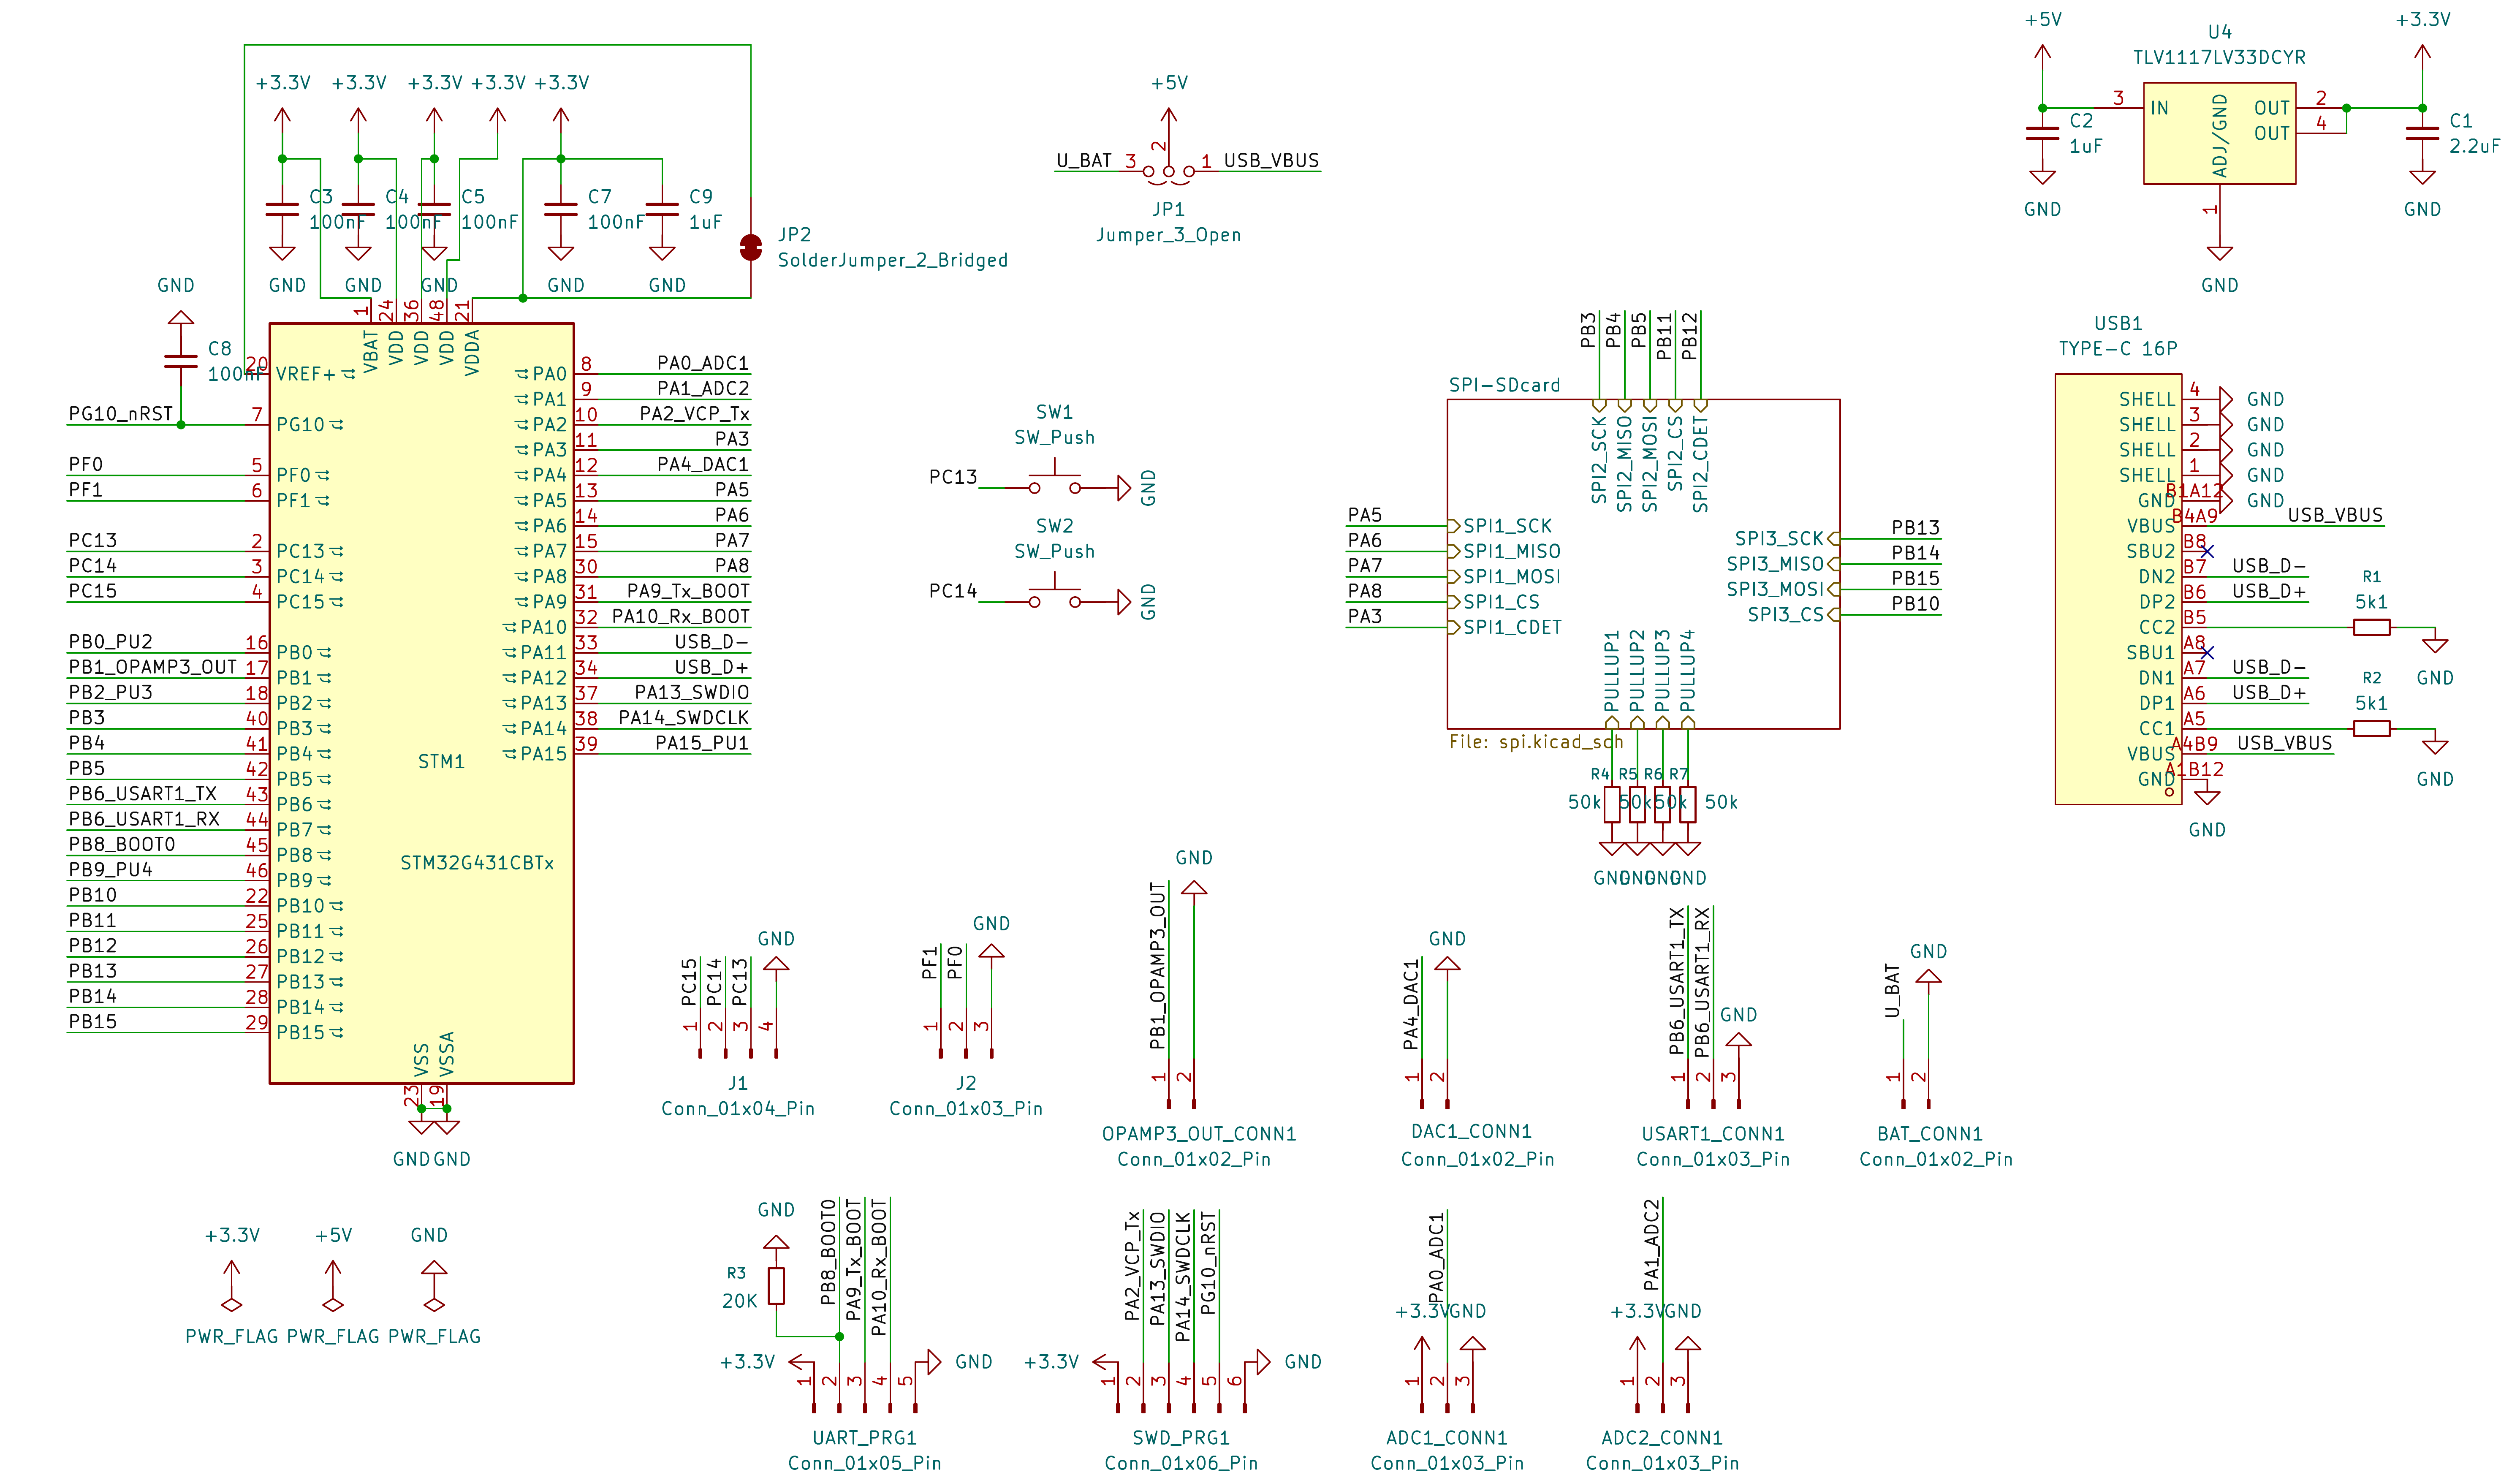
\includegraphics[width=1\linewidth]{Hard_Bilder/Schaltplan_main_highres.png}}
    \caption{Hauptblatt des Schaltplans}
    \label{fig:schalt_main}
\end{figure}
\fig{fig:schalt_main} zeigt den haupts"achlichen Schaltplan. In der Kurzschreibweise von Schaltungen werden oft die Leitungen
f"ur GND und VCC/VDD weggelassen. In "ahnlichem Stil wurden in dem vorliegenden Schaltplan fast alle anderen Leitungen auch
weggelassen und die Pins der "Ubersichtlichkeit halber mit Labels verbunden. Auch bei einem minimalen Design mussten einige 
Dinge f"ur eine korrekte Funktionsweise beachtet werden, andere Features wurden hinzugef"ugt, um eine bessere Auswertung
und Nutzung der Platine zu gew"ahrleisten.

\subsubsection{Spannungsversorgung}
Die Spannungsversorgung soll haupts"achlich "uber ein 5\,V USB-C-Netzteil gew"ahrleistet werden.
Ein umsteckbarer Jumper erm"oglicht allerdings auch die Versorgung "uber einen externen Akku,
sofern er minimal 3,8\,V bis 6\,V zur Verf"ugung stellt. Der STM32G431 ben"otigt an seinen
VDD-Pins allerdings 3,3\,V Spannung:
F"ur die Spannungsregelung
ist daher ein \texttt{Texas Instruments TLV1117LV33DCYR} Linearregler zust"andig. Dieser ben"otigt im Gegensatz zu vielen
Abw"artsreglern keine
komplexe, externe Beschaltung, sondern lediglich zwei Kondensatoren am Ein- und Ausgang. 
Weiterhin wurden f"ur eine stabile Spannungsversorgung alle VDD-Pins des STM32G431 mit 
einem 100 nF Kondensator ausgestattet.

\subsubsection{USB-C}
Die Platine ist mit einem 16-Pin USB Typ C Stecker ausgestattet. Da der Stecker beidseitig in die Buchse gesteckt werden kann,
ist jeder Pin in zweifacher Ausf"uhrung vorhanden.
Haupts"achlich ist der Stecker zur Spannungsversorgung gedacht gewesen. Damit die USB-Spannung von 5\,V von einem
Netzteil oder anderem Ger"at "uberhaupt bereitgestellt werden kann, m"ussen die Pins CC1 und CC2 "uber einen $5{,}1\kohm$ Widerstand
auf Masse gezogen werden. Es stehen mit USB-C auch h"ohere Spannungen zur Verf"ugung, wenn mit der Spannungsquelle "uber
das USB Power Delivery Protokoll kommuniziert wird. Dies war f"ur die vorliegende Arbeit aber nicht relevant. 

Da STM32G431 aber einen USB 2.0 Controller besitzt, wurden ebenfalls die differenziellen Datenpins angeschlossen.
Das erweitert die potenziellen M"oglichkeiten der Platine f"ur einen Datenaustausch mit dem Computer.

\subsubsection{SPI-Interfaces}
\begin{figure}[H]
    \centering
    \fbox{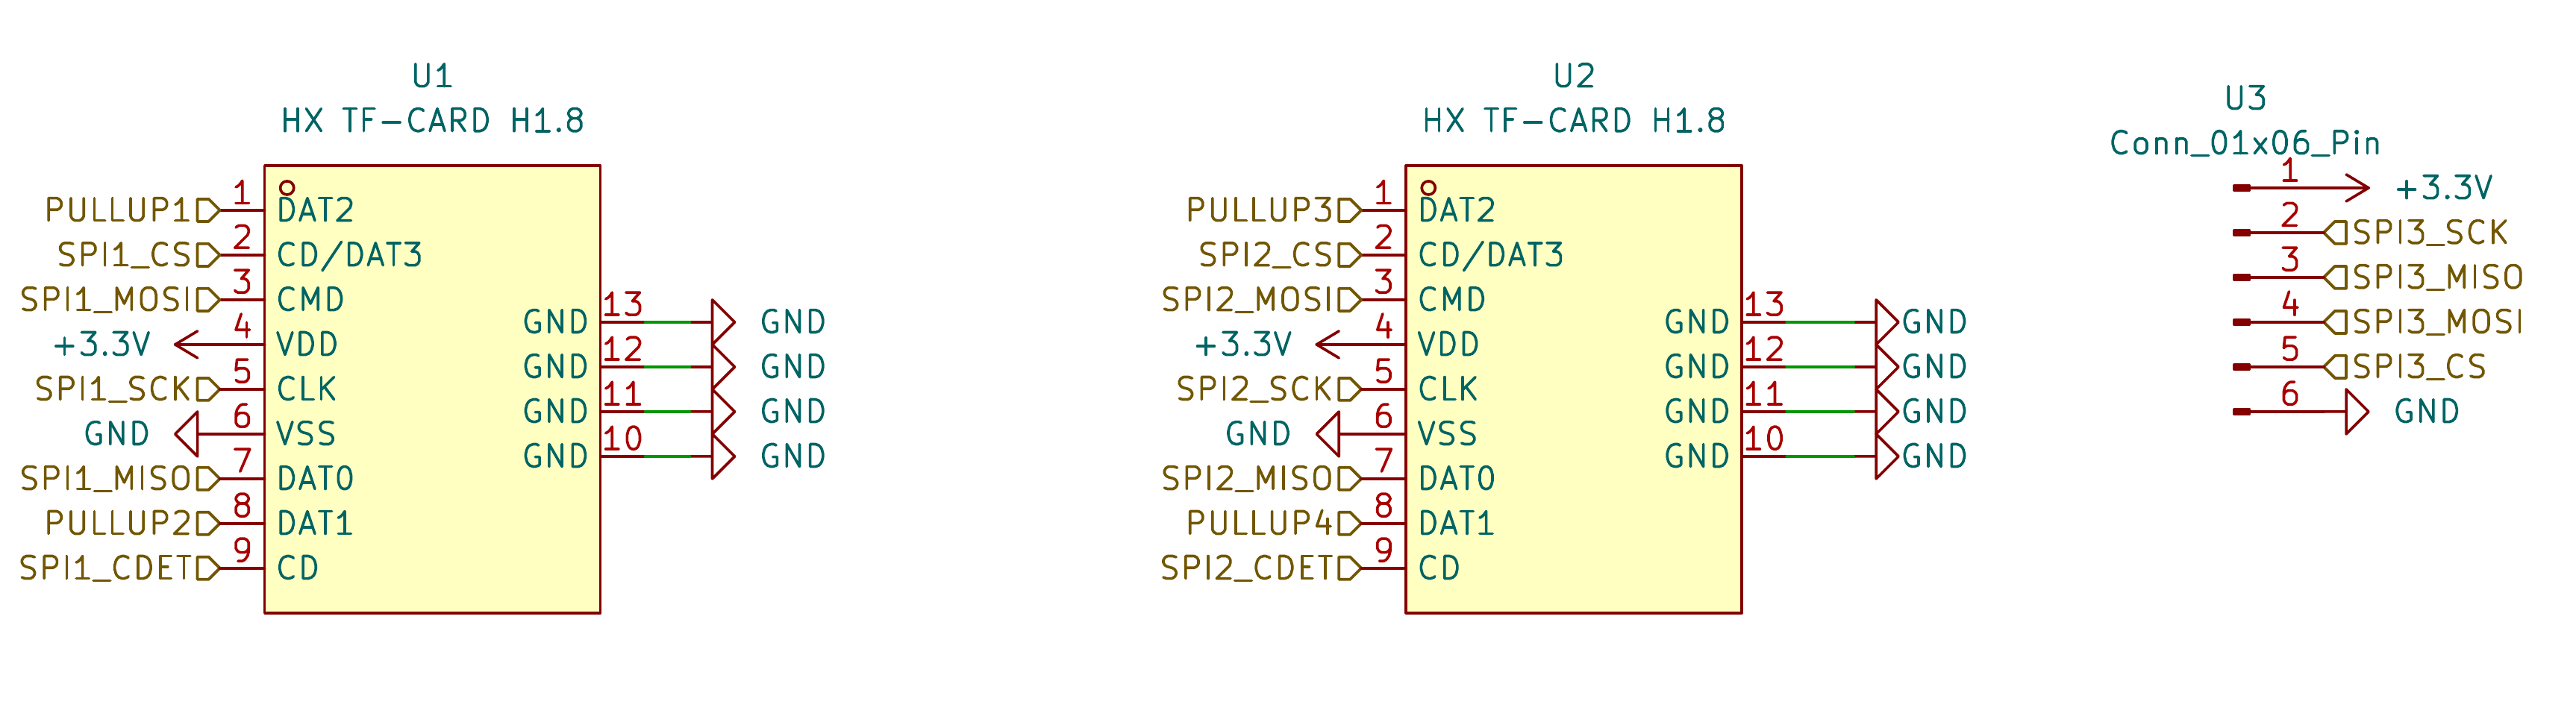
\includegraphics[width=1\linewidth]{Hard_Bilder/Schaltplan_spi_highres.png}}
    \caption{Schaltplan f"ur die SPI-Interfaces}
    \label{fig:schalt_spi}
\end{figure}
Die Hauptfunktionalit"at der Platine ist die Ansteuerung einer MicroSD-Karte "uber das SPI-Protokoll.
Der STM32G431 bietet hierf"ur eigene SPI-Hardwarecontroller, die als Master fungieren k"onnen und einen
konfigurierbaren Takt vorgeben. Die Platine verbindet zwei der drei SPI-Peripherien mit MicroSD-Karten Steckpl"atzen
und f"uhrt den dritten mit einer Pinleiste aus. Der gew"ohnliche Kommunikationsmodus von SD-Karten, der SD-Modus, ben"otigt
zwei weitere Pins. Diese werden in der vorliegenden Konfiguration aber per Pull-Up Widerstand auf 3,3 V Spannungspegel gebracht, 
um ein "Ubersprechen von den anderen Leitungen auf diese Pins zu unterbinden und damit potenzielle Fehler zu minimieren.
Die Pull-Up Widerst"ande sollten zun"achst direkt "uber ungenutzte STM32G431 Pins per Software konfiguriert werden.
Beim Routing hat sich dies jedoch als schwierig herausgestellt, sodass physische Pull-Up Widerst"ande verwendet werden sollten.
Durch die "Anderungen in letzter Minute hat sich hierbei allerdings ein Fehler eingeschlichen und die Widerst"ande sind
zu Pull-Down Widerst"anden geschaltet worden. 
Folglich muss die Prototypplatine ohne Pull-Up oder Pull-Down Widerst"ande genutzt werden.\\
Das dritte SPI-Interface wurde per Pinleiste herausgef"uhrt, sodass die Flexibilit"at gew"ahrleistet ist, ein
externes SPI-Ger"at anzuschlie"sen (wie z.B. einen kleinen LCD-Bildschirm), falls dies gew"unscht ist.

\subsubsection{Programmier-Interfaces}
Das Programmierinterface wurde in zwei Versionen herausgef"uhrt:\\
Einerseits das UART-Programmierinterface "uber eine 5-Pin Leiste.
Dieses erlaubt den STM32 "uber einen gew"ohnlichen UART-Adapter zu programmieren.
Der Nachteil ist hierbei allerdings, dass kein Debug-Interface vorhanden ist,
sodass die Entwicklung eines Programms erschwert wird. \\
Andererseits wurden die Pins f"ur das SWD-Interface mit einer 6-Pin Leiste herausgef"uhrt.
Dieses Interface ben"otigt einen dezidierten Programmieradapter. Allerdings lassen sich
mit einigen Jumperumstellungen auch die STM-Nucleo-Boards daf"ur nutzen,
da diese ebenfalls SWD intern f"ur ihre Programmierung verwenden. 
Zur Programmierung wurde ein NUCLEO-L053R8 verwendet, prinzipiell l"asst sich aber
jedes verf"ugbare Nucleo-Board verwenden.
N"aheres zu den Anschl"ussen findet sich beispielsweise im \href{https://www.st.com/resource/en/user_manual/um1724-stm32-nucleo64-boards-mb1136-stmicroelectronics.pdf}{User Manual UM1724} \cite{st4} ab Seite
17.


\subsubsection{VREF und ADCs/DACs}
Die ADC/DAC-Peripherie des STM32 ist f"ur den SD-Kartenversuch prinzipiell nicht notwendig,
erweitert die Funktionalit"at der Platine aber um potenzielle Ein- und Ausgabeoptionen und wurde
daher per Stiftleiste herausgef"uhrt.
F"ur die Referenzspannung der ADCs und DACs muss der Pin VREF mit VDDA verbunden werden und mit 
1\uF\ und 100 nF Kondensatoren abgesichert werden. Alternativ k"onnte man f"ur
eine Referenz den internen VREFBUF nutzen. In der vorliegenden Konfiguration besteht allerdings
maximale Flexibilit"at. Um die Komplexit"at der Schaltung niedrig zu halten, 
wurden in diesem Platinendesign keine separaten Versorgungen f"ur die digitale und analoge Spannung
verwendet, sodass mit einem h"oheren Grundrauschen bei den DACs und ADCs gerechnet werden muss. 
Es wurden 2x ADCs und 2x DACs "uber 2-Pin Leisten herausgef"uhrt. Einer der DACs ist intern
mit dem OPAMP3 verschaltet und somit gepuffert. 

\subsubsection{Weitere Peripherien}
F"ur potenzielle Debugging- und Kommunikationszwecke wurde ebenfalls per 3-Pin Leiste ein
USART-Interface herausgef"uhrt. F"ur eine einfache Eingabem"oglichkeit wurden zwei Pins
"uber einen Taster an GND angeschlossen. Diese sollen mit in Software zugeschalteten Pull-Up Widerst"anden
verwendet werden. Weiterhin wurden 5 weitere ungenutzte Pins herausgef"uhrt.



\subsection{Routing und Design}
\subsubsection{Footprints}
Da die Platine von Hand gel"otet werden sollte, wurden alle 
Kondensatoren und Widerst"ande in der 0805 Gr"o"se gew"ahlt.
Alle Bauteile wurden schon in der Schaltplanphase darauf begutachtet,
ob sie in einer von Hand l"otbaren Geh"auseform existieren. \\
Die Pads fast aller Bauteile wurden manuell etwas verl"angert, um
eine gute Handl"otbarkeit zu gew"ahrleisten.
LCSC stellt f"ur alle bei ihnen verf"ugbaren Bauteile auch Footprints
zur Verf"ugung. Die Footprints der spezielleren Bauteile, wie die des MicroSD-Kartenslots oder
des TI-Linearreglers, wurden mit dem Tool \href{https://github.com/uPesy/easyeda2kicad.py}{easyeda2kicad} in einen KiCad Footprint
"uberf"uhrt. Diese wiederum mussten teilweise auch leicht angepasst werden, weil z.B. 
der Abstand der Pads zu den Bohrl"ochern nicht die f"ur die Produktion zul"assigen Ma"se 
besessen hatte.

\subsubsection{Design}
\begin{figure}[H]
    \centering
    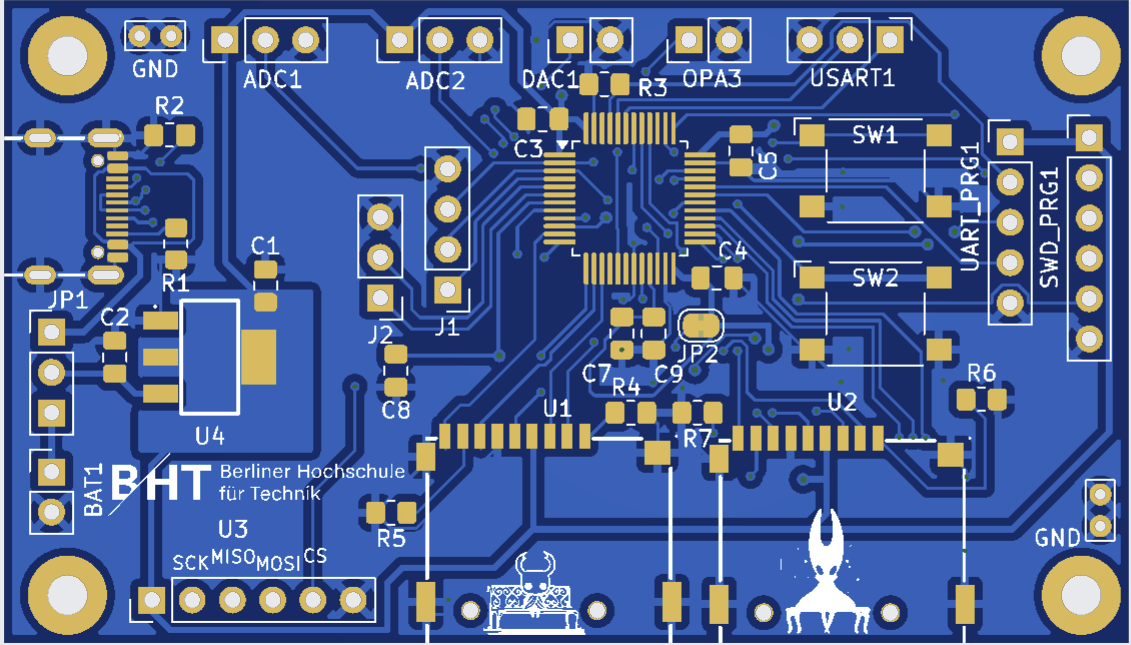
\includegraphics[width=1\linewidth]{Hard_Bilder/PreviewPCB.png}
    \caption{Vorschau der entwickelten PCB}
    \label{fig:platlayout}
\end{figure}
\fig{fig:platlayout} zeigt die Vorderseite der Platine in dem Zustand, in dem sie bestellt wurde.
Die Platine ist zweilagig angelegt und wird nur auf der Vorderseite per Hand best"uckt.\\
F"ur Signalleitungen wurden 0,2 mm dicke Kupferbahnen, f"ur die stromf"uhrenden Leitungen wurde 
eine Breite von 0,4 mm gew"ahlt. Der grundlegende Abstand von Leiterbahn zu Leiterbahn betr"agt 0,2 mm,
w"ahrend der Abstand zu nicht kontaktierten Bohrl"ochern 0,25 mm betr"agt. Dies sind "uberwiegend
Vorgaben des Produzenten JLCPCB. Die Gr"o"se der Platine betr"agt 71 mm x 40,5 mm.



Bei zuk"unftigen Projekten wird f"ur die Beschaltung das echte physische Layout der Pins
im Geh"ause st"arker beachtet werden. So liegen beispielsweise die Pins PA8 bis PA12 am
rechten oberen Rand des LQFP48-Geh"auses, w"ahrend die Pins PA0 bis PA4 in der linken unteren Ecke 
liegen. Dies ist beim Schaltungslayout irrelevant, beim Routing der echten Leitungen hingegen
f"uhrt dies zu "uberkreuzenden Leitungen. Daher sollte schon in der Schaltungsphase
das sp"atere physische Layout mitbedacht werden.  


\subsubsection{Fertigung}
Die bisherigen Ma"se und "Uberlegungen mussten schon konzeptionell und beim Entwurf im CAD-Programm beachtet werden.
F"ur die Fertigung bei JLCPCB mussten weitere Optionen festgelegt werden:
Der Materialtyp ist das "ubliche FR4 TG135 in der Farbe Blau. Die L"otpads werden nach dem Kupfer"atzprozess im \enquote{LeadFree HASL} Verfahren
mit einer Schutzschicht Zinn "uberzogen. Auf diese Option muss besonders geachtet werden, da in Asien
weiterhin bleihaltige Verzinnung "ublich ist. Diese Option ist vorteilhaft, da blankes Kupfer der Pads innerhalb kurzer Zeit oxidieren w"urde.
Die Kupferdicke liegt bei den "ublichen $35\um$. \\
Alle weiteren M"oglichkeiten sind Spezialoptionen f"ur Sonderanwendungen wie beispielsweise galvanisierte Kanten und sind f"ur diese Platine
nicht relevant.

\subsubsection{Best"uckung}
Die Best"uckung der Platine von Hand hat sich wie erwartet als gro"se Herausforderung dargestellt.
Vor allem das LQFP48 Geh"ause und der USB-C-Stecker konnten erst mit neu bestelltem NC-559 Flussmittel
richtig gel"otet werden. Stannol Flux X32-10i hingegen hat zu sehr vielen Br"ucken zwischen den Pins 
gef"uhrt. Weiterhin ist die Wahl der richtigen L"otspitze f"ur die Drag-Soldering-Technik entscheidend.
Entgegen der Intuition hat sich eine gr"o"sere L"otspitze als besser herausgestellt, weil diese die
Hitze, besonders in Kombination mit dem dickfl"ussigen Flussmittel, "uber eine gr"o"sere Fl"ache gleichm"a"siger 
verteilt.

\begin{figure}[H]
    \centering
    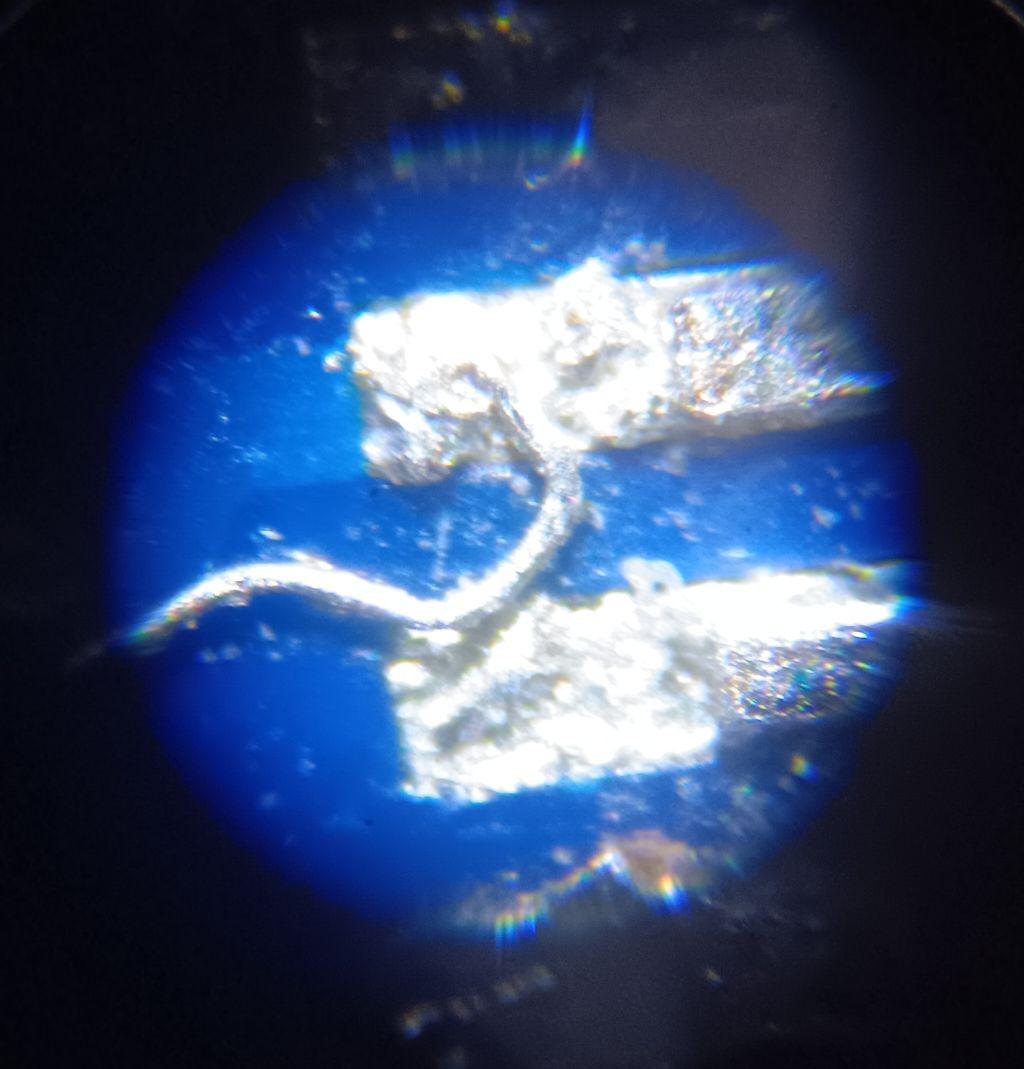
\includegraphics[width=0.55\linewidth, trim=0cm 2cm 0cm 2cm, clip]{Hard_Bilder/LQFP48_bruecke.jpg}
    \caption{L"otbr"ucke bei einem der LQFP48-Pins des STM32G431}
    \label{fig:loetproblem}
\end{figure}

\fig{fig:loetproblem} zeigt eine Mikroskopaufnahme einer ungewollten Br"ucke zwischen
zwei Pins, die durch das Benutzen von Entl"otlitze entstanden ist.
Ohne ein Mikroskop ist dieses Dr"ahtchen mit blo"sem Auge nicht zu sehen.

\begin{figure}[H]
    \centering
    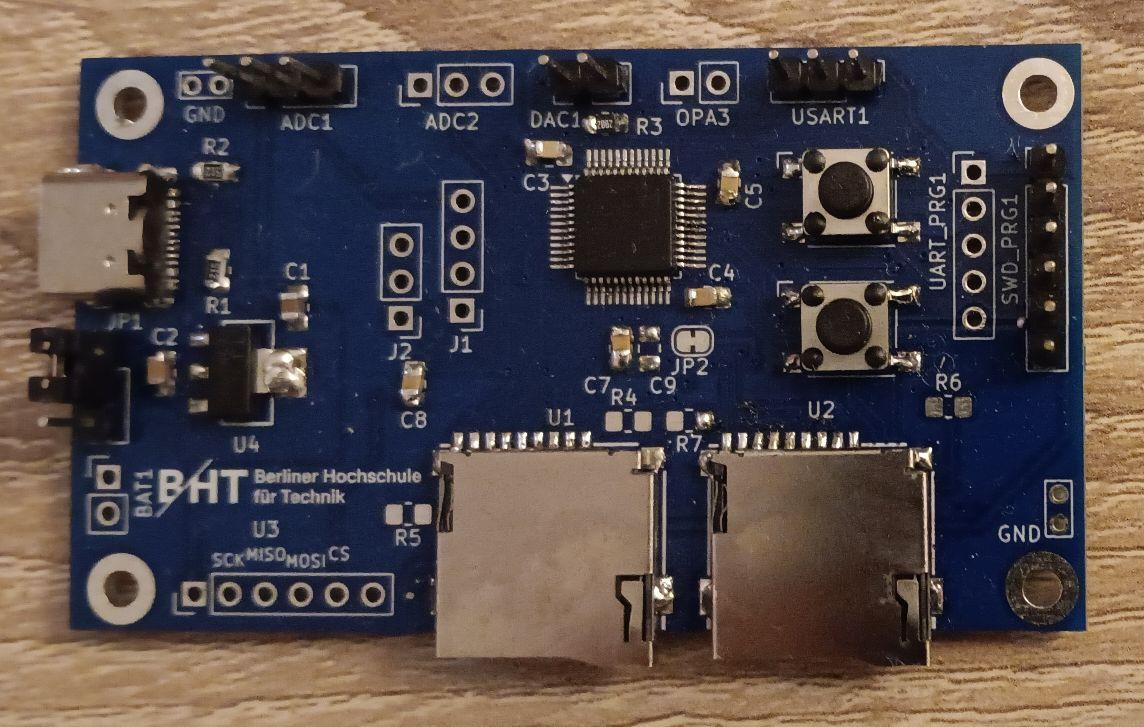
\includegraphics[width=0.8\linewidth]{Hard_Bilder/Platine_bestueckt.jpg}
    \caption{Platine in fast vollst"andiger Best"uckung}
    \label{fig:platbest}
\end{figure}
\fig{fig:platbest} zeigt eine der fertig gel"oteten Platinen.


\subsubsection{Inbetriebnahme und Probleme}
Neben dem bereits erw"ahnten Problem der falsch beschalteten Pull-Up Widerst"ande wurden ebenfalls
die Pins f"ur die SPI2 und SPI3 Peripherien vertauscht. Dieser Fehler l"asst sich durch eine 
Umkonfigurierung softwareseitig aber l"osen.\\
Der mit Abstand unintuitivste und am schwierigsten auszumachende Fehler der Platine h"angt 
allerdings mit der Spannungsversorgung f"ur die SD-Kartenslots zusammen. W"ahrend der Testungen
hat sich insbesondere der SD-Kartenslot, der an der SPI3-Peripherie angeschlossen ist, als 
besonders unzuverl"assig herausgestellt.\\
\fig{fig:misodip} zeigt den Kanal MISO, also die Antwort der SD-Karte auf eine Initialisierungsanfrage.
Die erwartete Antwort w"are 0xFF, also ein Signal, das durchgehend 3,3 V ist. Tats"achlich l"asst
sich aber eine kleine Kondensatorentladungskurve messen. Diese Entladungskurve war noch gr"o"ser,
als noch keine zus"atzlichen 2,2\uF\ Kondensatoren provisorisch in der N"ahe der SD-Kartenadapterversorgung gel"otet wurden.
Aber auch diese zus"atzlichen, provisorischen Kondensatoren sind nicht in der Lage, den Einbruch g"anzlich wegzupuffern.
Tats"achlich h"angt der Spike auch vom verwendeten Netzteil ab, auch wenn sich an der Spannungsversorgung
des Netzteils, sowie am TI-Linearregler, kein nennenswerter Einbruch messen l"asst.
Ohne einen 10 uF Kondensator ist der mit der SPI3 verbundene SD-Kartenslot daher leider nicht stabil benutzbar.
Dieser Fehler macht daher den SPI3 SD-Kartenslot unbenutzbar und l"asst sich ohne
ein neues Design kaum beheben.\\
Die Peripherie an SPI1 hingegen macht keine Probleme, vermutlich da sie sich physisch n"aher an der Spannungsversorgung
befindet und die Regelschleife des Linearreglers hier schnell genug die Versorgung nachregeln kann.

\begin{figure}[H]
    \centering
    \includegraphics[height=9cm]{Hard_Bilder/MISO_dip.png}
    \caption{MISO: SD-Kartenantwort auf CMD0}
    \label{fig:misodip}
\end{figure}


Ein schwer aufzufindbarer, leicht l"osbarer Fehler hing mit der Teilbest"uckung der Platine zusammen. F"ur
erste Tests wurde die Platine nicht vollst"andig mit allem best"uckt. So wurde der Widerstand R3
zun"achst vergessen zu l"oten. \fig{fig:schalt_main} macht deutlich, dass dies allerdings ein Pull-Down Widerstand 
f"ur den Boot-Pin PB8 ist.
Wenn sich PB8 auf HIGH befindet, so l"adt der STM32 in seinen internen Bootloader, um "uber
die UART-Schnittstelle programmierbar zu sein. Wenn der Pin allerdings unverbunden keinen
definierten Pegel erh"alt, so l"adt er mal in den Bootloader und mal nicht, sodass sich die
Platine in einem schwer diagnostizierbaren Zustand befindet. 


\subsection{Fazit}

Alles in allem ist das Design f"ur einen ersten Prototypen sehr gelungen und funktional.
Der STM32 wird stabil mit Spannung versorgt und l"asst sich "uber ein speziell konfiguriertes Nucleo-Board
debuggen und programmieren.
Die SPI1- und mit Einschr"ankungen auch die SPI3-Peripherien lassen sich f"ur die weitere Arbeit verwenden. 
Eine wichtige Erkenntnis ist, dass schon beim Schaltungsdesign das sp"atere Layout mitbedacht werden muss,
um vorausschauende Entscheidungen bez"uglich der Pinwahl treffen zu k"onnen.\\
SD-Karten scheinen durch ihren internen Aufbau kurzfristig hohe Stromspitzen zu verursachen,
die der verwendete LDO-Regler vermutlich aufgrund der r"aumlichen Entfernung des Bauteiles nicht ausregeln kann. 
Daher ist es g"unstig, diese in der N"ahe der Spannungsversorgung zu platzieren und mit dezidierten Kondensatoren
auszustatten. \\
Ein gro"ses "Argernis bei der Fehlersuche, insbesondere im Hinblick auf die SPI-Peripherie, die die Grundlage
des SD-Kartentreibers bildet, ist eine fehlende Pinleiste f"ur das Debugging. Ohne diese war es nur
mit gr"o"ster M"uhe und Pr"azision m"oglich, einzelne SPI-Pins mit dem Oszilloskop zu messen. Ein Anschluss
an einen Logikanalyser w"are hingegen gar nicht m"oglich gewesen. Weiterhin wurde zwar "uberwiegend mit einem Debugger gearbeitet, 
für viele der in den weiteren Arbeit durchgef"uhrten Versuche w"are eine Status-LED dennoch sehr praktisch gewesen. \\
All diese Punkte w"aren in einer zweiten Version der Platine aber leicht nachzubessern. 

\subsection{Testhardware}
Bestellungen aus China ben"otigen mehrere Wochen Zeit.

\MP{b}{0.5}{
    \begin{figure}[H]
        \centering
        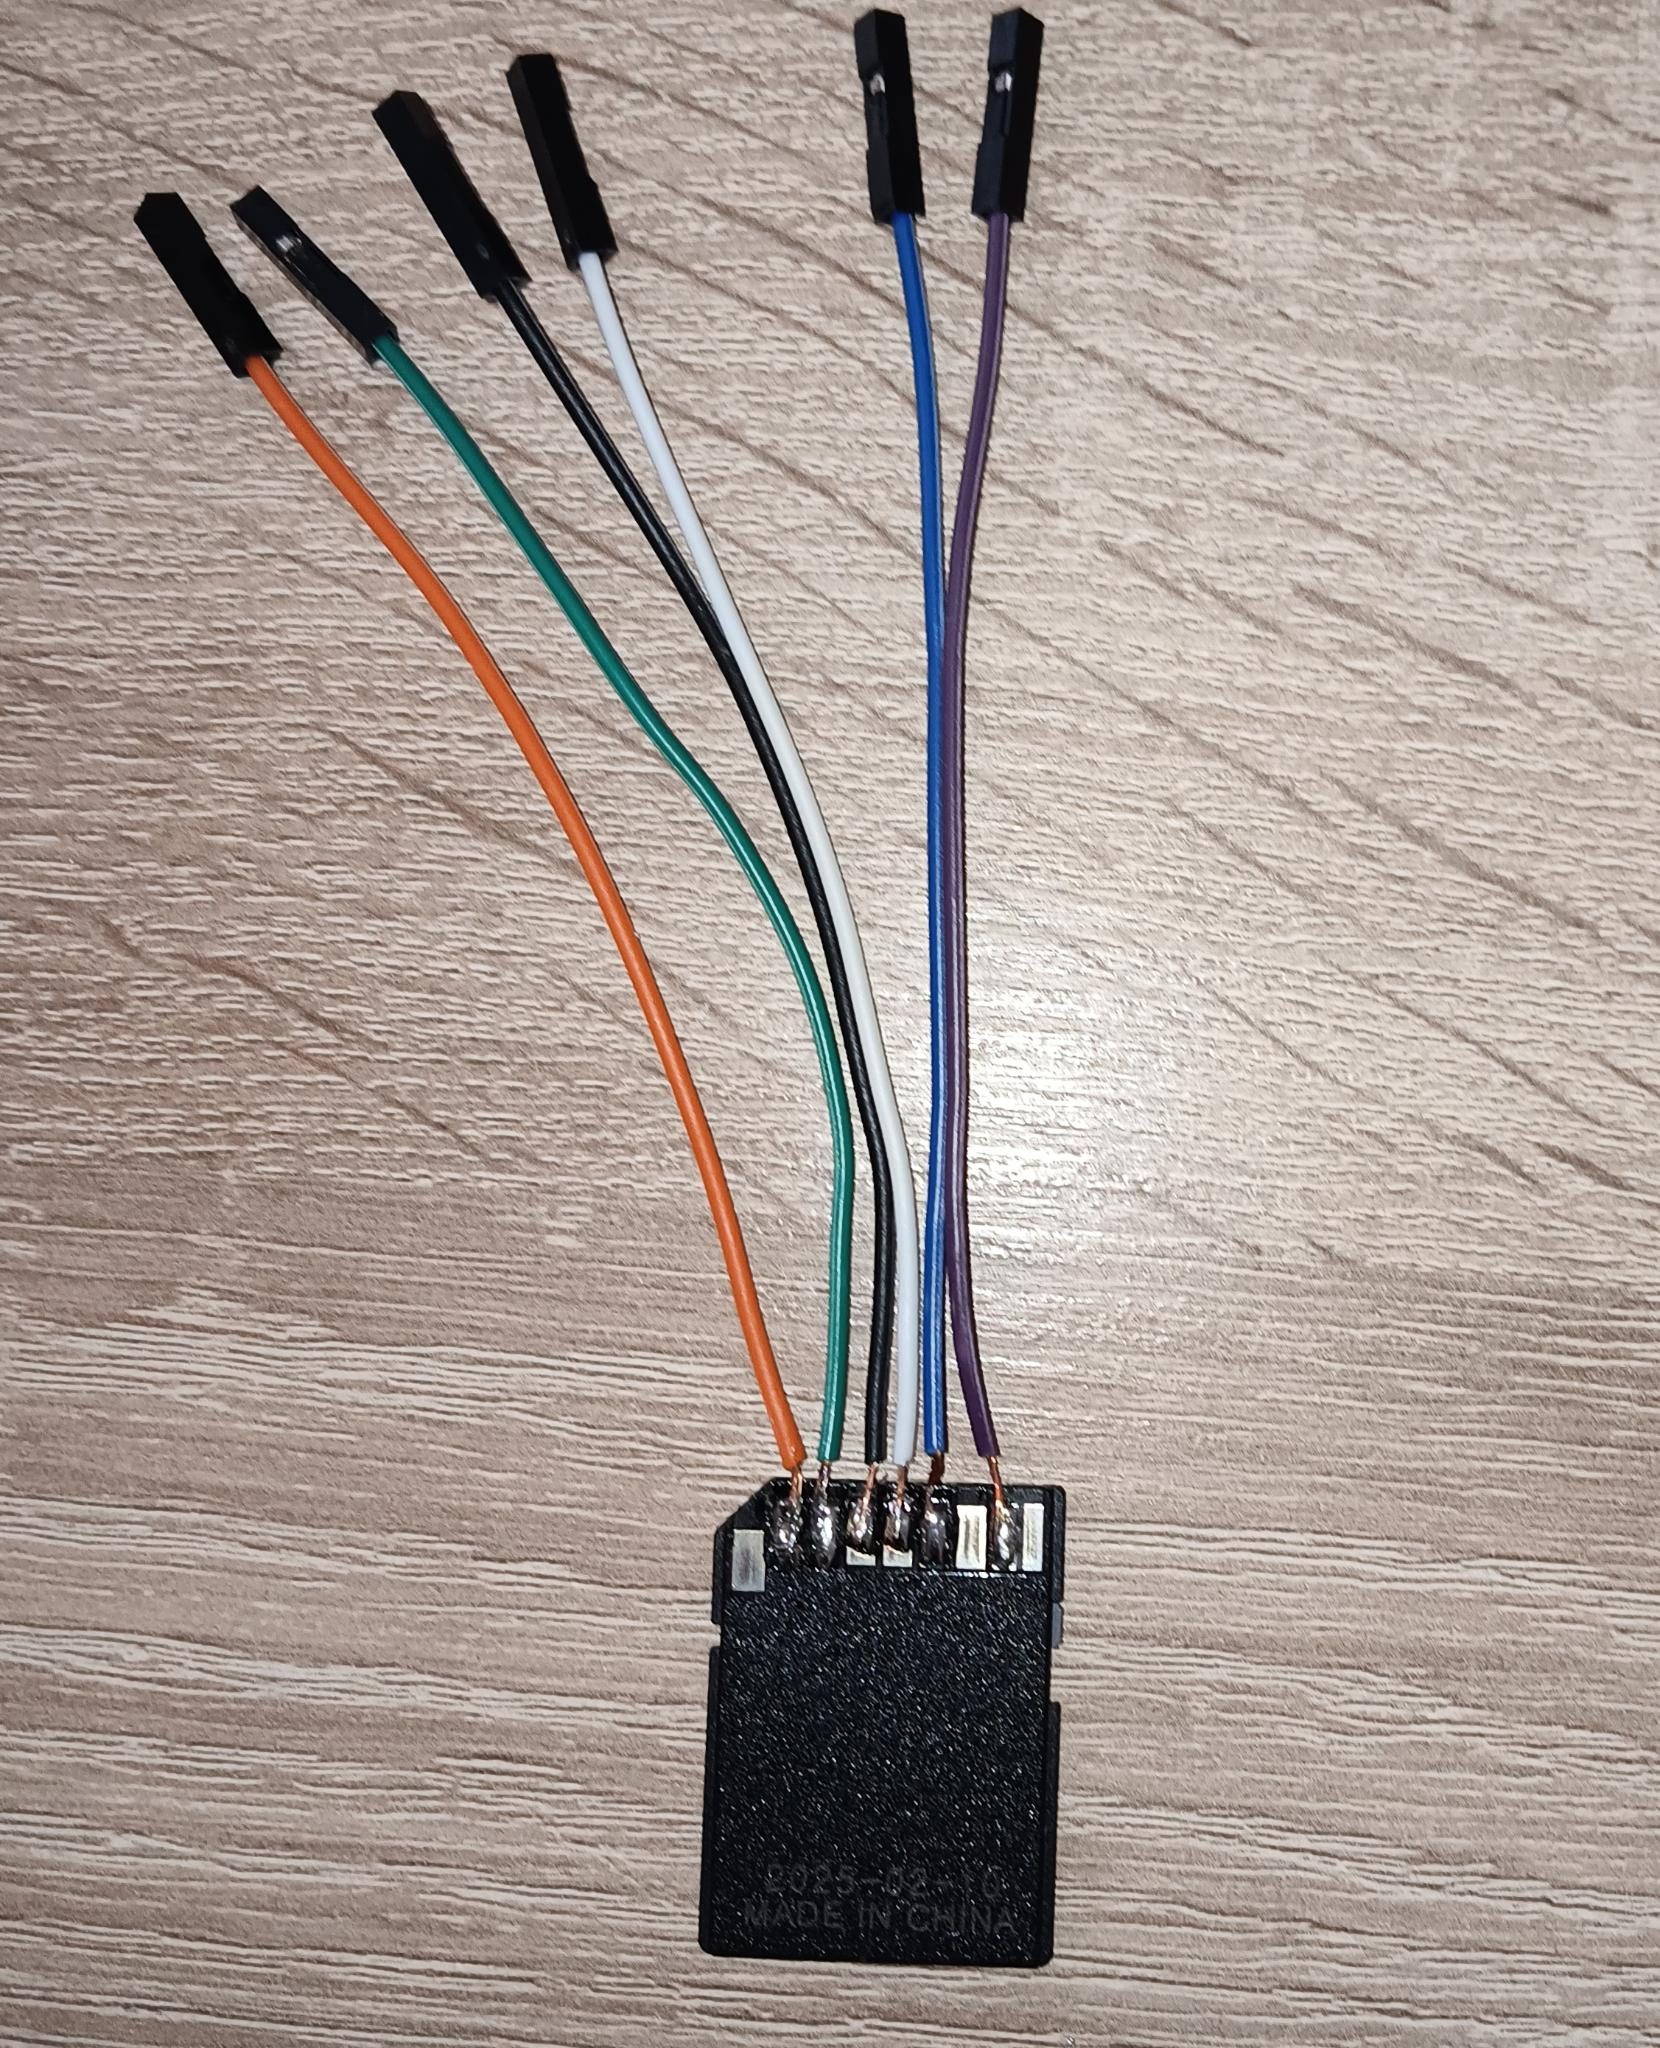
\includegraphics[height=6cm]{Hard_Bilder/sdadapter_sold.jpg}
        \caption{Erster gel"oteter SD-Adapter}
        \label{fig:sd_sold}
    \end{figure}
}
\MP{b}{0.5}{
    \begin{figure}[H]
        \centering
        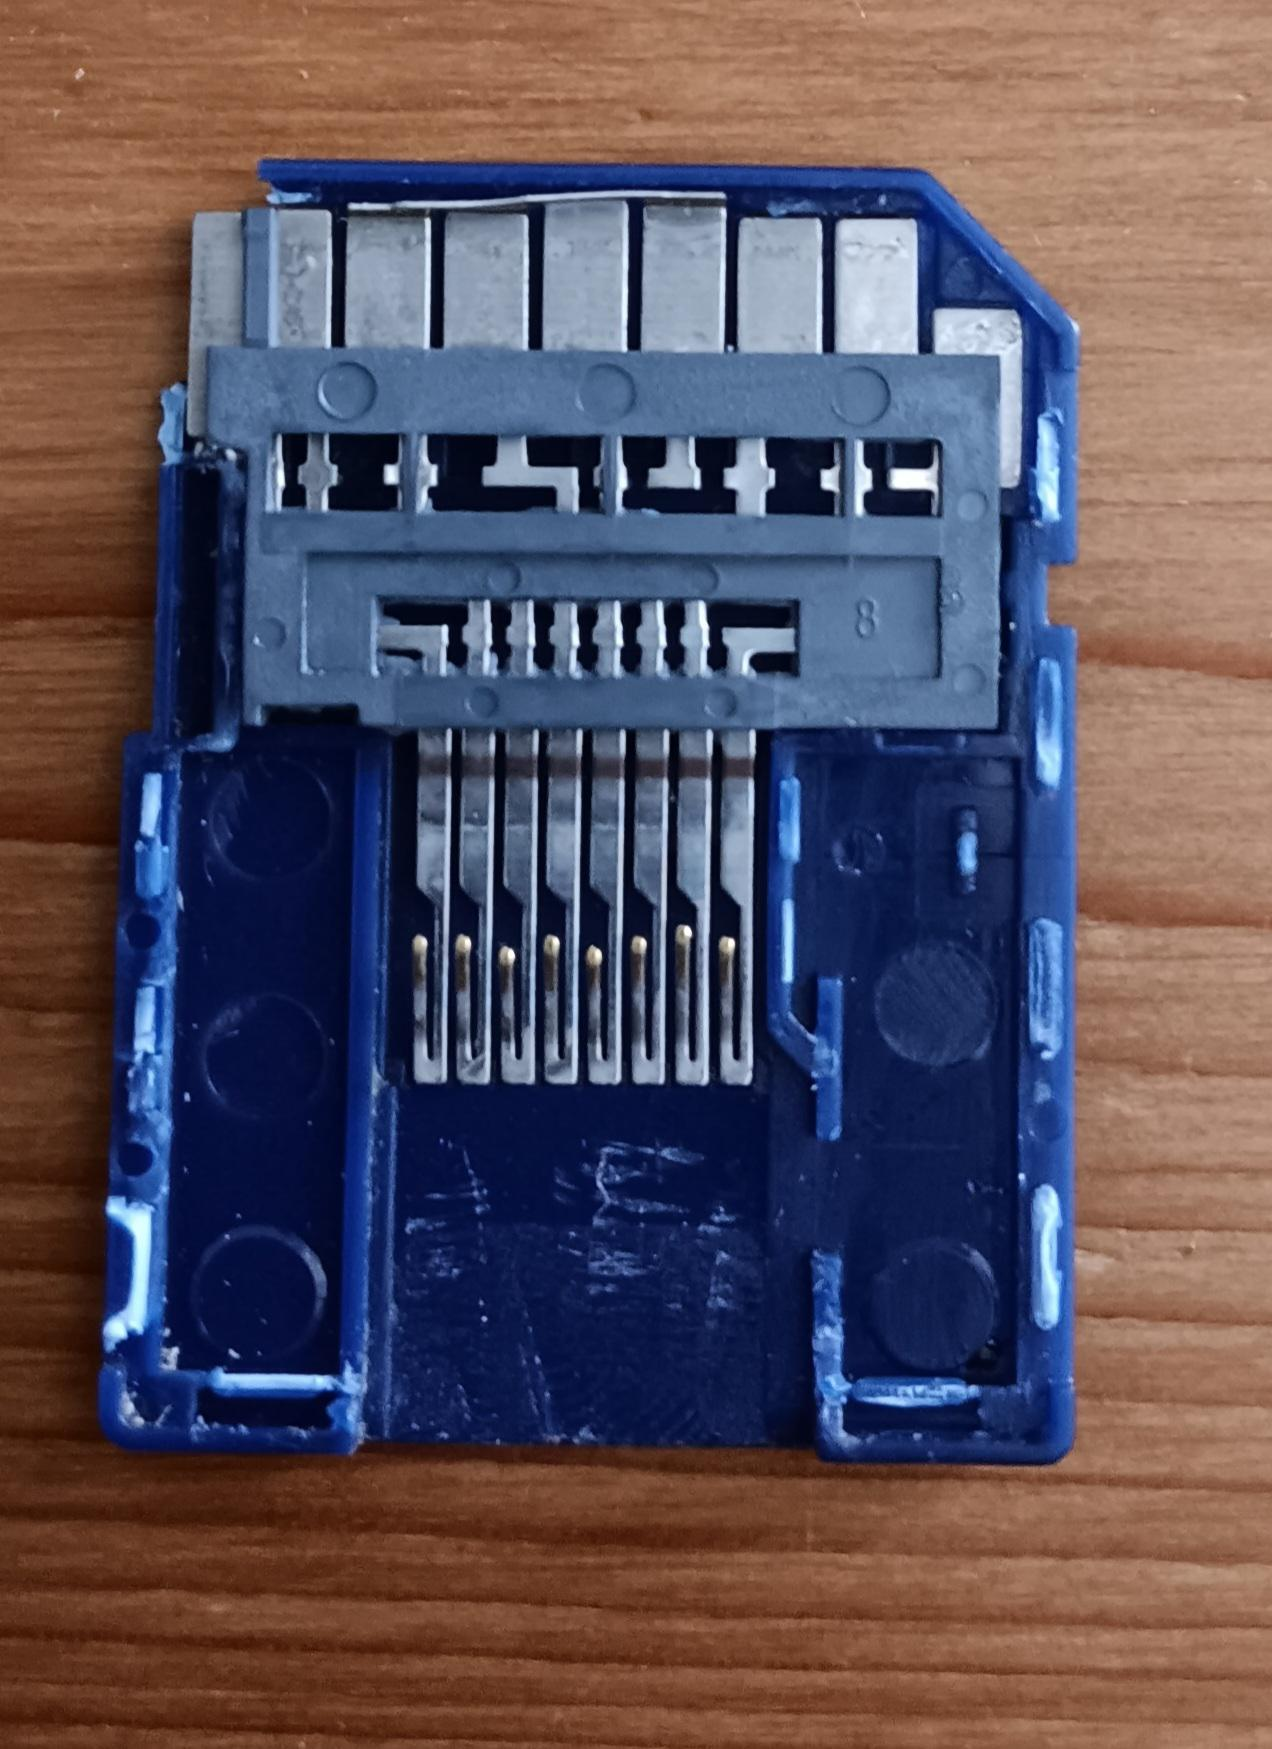
\includegraphics[height=6cm]{Hard_Bilder/sdadapter_broken.jpg}
        \caption{Aufgebrochener SD-Adapter}
        \label{fig:sd_broken}
    \end{figure}
}


Um in der Zwischenzeit an der Arbeitsstellung weiterarbeiten zu k"onnen,
wurde der in \fig{fig:sd_sold} gezeigte Adapter in Kombination
mit einem ST NUCLEO-G431RB verwendet. Diese Adapter finden sich meist bei jeder gekauften MicroSD-Karte
und haben den Zweck, die kleine Karte in ein gr"o"seres Format zu "uberf"uhren.
Die improvisierte L"osung erwies sich jedoch nicht als sehr zuverl"assig:
Schon nach zwei Wochen musste ein neuer Adapter, diesmal mit gecrimpten Aderendh"ulsen, gel"otet werden,
da sich einzelne Str"ange des Litzenkabels gel"ost hatten und zu Kurzschl"ussen gef"uhrt hatten.


\section{SPI- und SD-Karten-Treiber} \label{sec:spi} 

\subsection{Entwicklungsumgebung und Embedded C++20}
F"ur die Entwicklung des SPI- und SD-Karten-Treibers wurde bewusst auf modernes C++20 zur"uckgegriffen.
Die Sprache erlaubt Hardware-Abstraktionen mit Templates und Berechnungen zur Compilezeit mit \cpp{constexpr} 
vollkommen ohne Laufzeitoverhead, sogenannte Zero-Cost-Abstractions.
Moderne Sprachfeatures wie \cpp{enum class} und \cpp{namespace} bieten Typensicherheit und erh"ohen die Lesbarkeit.
Bedingte Kompilierung mit \cpp{if constexpr} w"ahlt nur relevante Zweige zur Compilezeit aus und kompiliert den Rest erst gar nicht.
Gleichzeitig besteht Abw"artskompatibilit"at zu C-Code, sodass beispielsweise die in C89 geschriebene
FatFS-Bibliothek problemlos eingebunden werden kann.\\
Weiterhin wurde f"ur die Entwicklungsumgebung bewusst auf die STM32CubeIDE verzichtet und stattdessen ein Setup aus CMake und VS Code verwendet.
Dadurch bleibt der Buildprozess unabhängig von einer spezifischen IDE 
und kann flexibel angepasst werden.
CMake ermöglicht zudem eine einfache Automatisierung des Builds: F"ur die vorliegende
Arbeit wurden zahlreiche sehr kurze Testprogramme entwickelt. Bei einer "Anderung einer
geteilten Quelldatei wurden automatisch alle betroffenen Programme neu kompiliert.
VS Code bietet dabei eine schlanke und flexibel erweiterbare Entwicklungsumgebung.
So konnte für die cpp-Quelldateien, 
die tex-Dateien dieser Arbeit und die Rohdaten 
derselbe Editor verwendet werden.
Die Programmierung und das Debugging des STM32 sind mit entsprechenden Erweiterungen direkt
aus dem Editor m"oglich.
%namespace problematik schreiben, folgender Fehler:
% [build]  1130 | #define CRC                 ((CRC_TypeDef *) CRC_BASE)
% [build]       |                              ~            ^
% [build] /home/alle/Universitaet/BA-stm/FatFS/spi-sdcardwrite/src/sdcarddriver.hpp:556:13: note: in expansion of macro 'CRC'
% [build]   556 |     uint8_t CRC : 7;                  // [7:1]

\subsection{GPIO HAL}
Um nicht st"andig direkte und dadurch schwer lesbare Registerzugriffe
 innerhalb der Treiber vornehmen zu müssen, wurde eine kleine Zero-Cost-Abstraction
für die Konfiguration und Ansteuerung der GPIOs implementiert.
Die in \texttt{src/GPIO\_HAL.hpp} verwendete Template-Klasse \cpp{GpioPin} 
erh"alt die Basisadresse des verwendeten GPIO-Ports sowie die Pinnummer als Compilezeit-Parameter. 
Dadurch k"onnen konkrete GPIO-Pins typsicher beschrieben
und über eine einheitliche Schnittstelle konfiguriert werden.
Die Klasse stellt unter anderem Funktionen zur Konfiguration als Ein- oder Ausgang, 
zur Auswahl von Pull-Up- bzw. Pull-Down-Widerständen sowie zur Konfiguration von Alternate Functions bereit.
Da Port und Pin bereits zur Compilezeit feststehen und die bereitgestellten Funktionen als \cpp{static} implementiert sind,
ist zur Laufzeit keine Objektinstanz erforderlich. 
Bei entsprechender Compileroptimierung können die Methoden daher auf die für den jeweiligen Pin notwendigen direkten Registerzugriffe reduziert werden. 
Die Abstraktion dient somit prim"ar der Lesbarkeit und Wartbarkeit des Quellcodes, ohne einen relevanten Laufzeit- oder Speicher-Overhead einzuführen.
\begin{listing}[H]
    \begin{minted}[
        frame=lines,      % Rahmenlinien oben und unten
        framesep=2mm,     % Abstand zum Rahmen
        baselinestretch=1.2,
        bgcolor=lightgray!20, % Hintergrundfarbe
        fontsize=\footnotesize,
        linenos           % Zeilennummern aktivieren
    ]{cpp}
    static void AF(uint8_t af)
    {
        // Alternate function mode
        GPIOx->MODER &= ~(0b11 << (Pin * 2));
        GPIOx->MODER |=  (0b10 << (Pin * 2));

        // AFRL or AFRH
        if constexpr (Pin < 8)
        {   
            
            GPIOx->AFR[0] &= ~(0xF << (Pin * 4));
            GPIOx->AFR[0] |=  (static_cast<uint32_t>(af) << (Pin * 4));
        }
        else
        {
            constexpr uint32_t shift = (Pin - 8) * 4;
            GPIOx->AFR[1] &= ~(0xF << shift);
            GPIOx->AFR[1] |=  (static_cast<uint32_t>(af) << shift);
        }
    }
    \end{minted}
\caption{if constexpr bei der Alternate Function Implementation}
\label{listing:AF}
\end{listing}

\coderef{listing:AF} zeigt beispielhaft den Code f"ur die Implementierung der Alternate Function.
Hier gestaltet sich \cpp{if constexpr} vorteilhaft, da die Pinnummer Pin bereits zur Compile-Zeit als Template-Parameter bekannt ist. 
Dadurch wird nur der tatsächlich benötigte Zweig für AFR[0] oder AFR[1] kompiliert, während der andere Zweig vollständig entfällt.


\subsection{Debugging mit GDB}
Ein absolut wesentlicher und sehr zeitintensiver Teil der Arbeit ist das Debugging der Hard- und Software.
Zum Debugging wurde die VS Code Erweiterung \href{https://marketplace.visualstudio.com/items?itemName=marus25.cortex-debug}{Cortex-Debug}
verwendet. Diese nutzt im Hintergrund den \href{https://www.sourceware.org/gdb/}{GNU Project Debugger (GDB)}. \\
Mit der Erweiterung und der richtigen .svd Datei f"ur den STM32G431 lassen sich direkt aus dem Editor Programme 
auf den STM32 flashen und Register und Variablen auslesen. Durch die Nutzung von CMake lassen sich au"serdem
bequem mehrere ausf"uhrbare Programme kompilieren und leicht wechseln.\\
So war recht schnell erreicht, dass das Projekt eine f"ur das direkte Auslesen
von Variablen unhandliche Gr"o"se angenommen hat. 
F"ur das Debugging wurde diese Arbeit vom Rustprojekt \href{https://defmt.ferrous-systems.com/}{defmt} inspiriert,
das Debuggingnachrichten direkt "uber die Debug-Probe ST-Link ohne einen zus"atzlichen UART-Kanal oder
den SWO-Pin senden kann. Dies ist besonders n"utzlich, da der ST-Link zum Flashen der Programme ohnehin am 
Mikrocontroller angeschlossen sein muss. \\ 
Die minimale L"osung f"ur diese Arbeit nutzt letztlich aus, dass GDB im angehaltenen Zustand immer den Speicher des
Mikrocontrollers auslesen kann. Damit ist es m"oglich, f"ur Testprogramme GDB-Skripte zu entwerfen, die
bestimmte Flags von Variablen oder ganze Variablen auswerten.


\begin{listing}[H]
    \begin{minted}[
        frame=lines,      % Rahmenlinien oben und unten
        framesep=2mm,     % Abstand zum Rahmen
        baselinestretch=1.2,
        bgcolor=lightgray!20, % Hintergrundfarbe
        fontsize=\footnotesize,
        linenos           % Zeilennummern aktivieren
    ]{cpp}
    define spi_test
    printf "\n\n SD Card Test:\n\n"

    ###SPI1###
    if sdtest.cur_spi == 1
        printf "TESTING SPI1 PERIPHERAL \n"

        #CARD DETECT
        if sdtest.carddetect == 1
            printf "SPI1: CARD NOT DETECTED [FAILED]"
        end
        if sdtest.carddetect == 0
            printf "SPI1: CARD DETECTED [OK]"
        end

        #SD CARD INIT
        if sdtest.initsd == SD_INIT_OK
            printf "SPI1: SD CARD INIT [OK]\n"
        end
        if sdtest.initsd == 0x02
            printf "SPI1: SD CARD INIT [FAILED: 0x02] => CMD0 FAILED\n"
        end
        if sdtest.initsd == 0x04
            printf "SPI1: SD CARD INIT [FAILED: 0x04] => CMD8 FAILED\n"
        end
        if sdtest.initsd == 0x08
            printf "SPI1: SD CARD INIT [FAILED: 0x08] => TIMEOUT: CMD55 + ACMD41 LOOP FAILED\n"
        end
        (...)
    end
    \end{minted}
\caption{Auszug aus \texttt{test/spi\_test.gdb}}
\label{listing:gdbdebug1}
\end{listing}


\coderef{listing:gdbdebug1} zeigt einen Auszug aus dem erstellten GDB-Skript, welches die beiden SD-Kartenslots
auf ihre Funktionsf"ahigkeit pr"uft.\\
Die dazugeh"orige, typische Ausgabe in der GDB-Debug-Konsole zeigt \coderef{listing:gdbdebugausgabe}.
Damit lässt sich mit einem Durchlauf des Programms feststellen, ob die zugrundeliegenden
Funktionen des SPI/SD-Treibers alle ordnungsgemä"s funktionieren und ob die Karte sich mit 
einem der beiden Dateisysteme mounten l"asst und ob die grundlegenden Funktionen des Dateisystems, wie zum Beispiel das Lesen und Schreiben, fehlerfrei ausf"uhrbar sind.



\begin{listing}[H]
    \begin{minted}[
        frame=lines,      % Rahmenlinien oben und unten
        framesep=2mm,     % Abstand zum Rahmen
        baselinestretch=1.2,
        bgcolor=lightgray!20, % Hintergrundfarbe
        fontsize=\footnotesize,
        linenos           % Zeilennummern aktivieren
    ]{text}
     SD Card Test:
    TESTING SPI1 PERIPHERAL
    SPI1: CARD DETECTED [OK]
    SPI1: SD CARD INIT [OK]
    SPI1: SD CARD WRITE SINGLE BLOCK [OK]
    SPI1: SD CARD READ SINGLE BLOCK [OK]
    SPI1: SD CARD READ MULTIPLE BLOCK [OK]
    SPI1: SD CARD WRITE MULTIPLE BLOCK [OK]
    SPI1: READ SINGLE BLOCK SAME AS WRITTEN [OK]
    SPI1: READ MULTIPLE BLOCK SAME AS WRITTEN [OK]
    SPI1: GOT CSD [OK]
    SPI1: CARD SIZE IN MB: 31268
    SPI1, FatFS: MOUNT [FAILED]
    SPI1, FatFS: FOPEN [FAILED]
    SPI1, FatFS: FWRITE [FAILED]
    SPI1, FatFS: CLOSE [FAILED]
    SPI1, littlefs: INIT [OK]
    SPI1, littlefs: FORMAT [NONE]
    SPI1, littlefs: MOUNT [OK]
    SPI1, littlefs: OPEN [OK]
    SPI1, littlefs: WROTE 32 BYTES
    SPI1, littlefs: REWIND [OK]
    SPI1, littlefs: READ 32 BYTES
    SPI1, littlefs: READBUFFER IS SAME AS WRITEBUFFER [OK]
    SPI1, littlefs: CLOSE [OK]
    SPI1, littlefs: UNMOUNT [OK]
    \end{minted}
\caption{Debugausgabe von \texttt{test/spi\_test.cpp} durch Anwendung von \texttt{spi\_test.gdb}}
\label{listing:gdbdebugausgabe}
\end{listing}


GDB-Skripte sind ebenfalls in der Lage Breakpoints zu setzen. Mit dieser Funktion l"asst sich 
ein einfaches Debug-Print in der GDB-Debug-Konsole realisieren.
\coderef{listing:gdbdebug2} zeigt einen weiteren Auszug aus dem erstellten GDB-Skript \texttt{spi\_test.gdb}.
Dieser Code setzt einen Breakpoint bei der Funktion \cpp{debug_gdb_print} und gibt dessen str-Variable aus.
\coderef{listing:gdbdebug3} zeigt den vollst"andigen Code der Funktion \cpp{debug_gdb_print}. Mit dieser
Kombination ist es m"oglich, die Funktion im Code aufzurufen. Diese macht codetechnisch nichts, veranlasst
den Debugger aber kurz bei ihr anzuhalten, die Variable str auszugeben und sofort den Programmablauf fortzuf"uhren.
W"ahrend diese Funktionalit"at nicht in zeitkritischen Schleifen zum Einsatz kommen kann, ist sie f"ur
allgemeine Debuggingnachrichten sehr gut anwendbar. Gleichzeitig ist kein zus"atzliches, externes Modul
notwendig, sondern die bereits vorhandenen Funktionalit"aten des GDB-Debuggers k"onnen ausgenutzt werden. 

\begin{listing}[H]
    \begin{minted}[
        frame=lines,      % Rahmenlinien oben und unten
        framesep=2mm,     % Abstand zum Rahmen
        baselinestretch=1.2,
        bgcolor=lightgray!20, % Hintergrundfarbe
        fontsize=\footnotesize,
        linenos           % Zeilennummern aktivieren
    ]{cpp}
void debug_gdb_print(const char* str)
{
    // breakpoint target only
}
    \end{minted}
\caption{Auszug aus \texttt{test/sd\_test.cpp}}
\label{listing:gdbdebug3}
\end{listing}

\begin{listing}[H]
    \begin{minted}[
        frame=lines,      % Rahmenlinien oben und unten
        framesep=2mm,     % Abstand zum Rahmen
        baselinestretch=1.2,
        bgcolor=lightgray!20, % Hintergrundfarbe
        fontsize=\footnotesize,
        linenos           % Zeilennummern aktivieren
    ]{cpp}
    break debug_gdb_print
    commands
        printf "%s", str
        continue
    end
    \end{minted}
\caption{Auszug aus \texttt{test/spi\_test.gdb}}
\label{listing:gdbdebug2}
\end{listing}








\subsection{SPI}

\subsubsection{Anschlussbelegung}

\begin{table}[H]
    \centering
    \caption{Anschlussbelegung der Standard SD-Karte am STM32G431 im SPI-Modus f"ur SPI1}
    \label{tab:standardsd_spi}
    \begin{tabular}{lllll}
    \toprule
    \textbf{Pin} & \textbf{SD-Modus} & \textbf{SPI-Modus} & \textbf{Beschreibung (SPI)} & \textbf{STM32G431 Pin} \\ \midrule
    1            & DAT3 / CD         & CS        & Chip Select (Low-aktiv)     & GPIO (hier PA8)        \\
    2            & CMD               & DI        & Data In (Dateneingang)      & PA7 (MOSI)              \\
    3            & VSS1              & VSS       & Masse                       & GND                     \\
    4            & VDD               & VDD       & Spannungsversorgung (3,3\,V)    & 3,3\,V                  \\
    5            & CLK               & SCLK      & Taktleitung                 & PA5 (SCK)               \\
    6            & VSS2              & VSS       & Masse                       & GND                     \\
    7            & DAT0              & DO        & Data Out (Datenausgang)     & PA6 (MISO)              \\
    8            & DAT1              & \textit{Nicht genutzt} & Pull-Up/nicht belegt                & --                      \\
    9            & DAT2              & \textit{Nicht genutzt} & Pull-Up/nicht belegt                 & --                      \\ \bottomrule
    \end{tabular}
\end{table}

\tab{tab:standardsd_spi} verdeutlicht die Anschlussbelegungen f"ur eine SD-Karte in Standardgr"o"se, wie sie f"ur die Testhardware
am NUCLEO-G431RB verwendet wurden. Au"serdem verdeutlicht die Tabelle die Funktionen der einzelnen Pins der SD-Karte.
Hier zeigt sich auch, dass eine SD-Karte im SD-Modus bis zu 4 Datenleitungen nutzen kann, w"ahrend sie im SPI-Modus nur
eine nutzt. Dadurch sind im SD-Modus selbstverst"andlich h"ohere Datenraten m"oglich, w"ahrend sich der SPI-Modus
durch eine einfachere Handhabung auszeichnet.

\fig{fig:sd_broken} verdeutlicht, dass SD-Adapter lediglich die Leitungen der MicroSD-Karte umlenken.
Die angewandten Belegungen f"ur eine MicroSD-Karte, mit der auch die Platine arbeitet, finden sich in \tab{tab:microsd_pinout}.
Es besteht eine gewisse Variabilit"at, welche Pins f"ur welche SPI-Peripherie genutzt werden.
Dies wird anhand der zugeh"origen Alternate Functions entschieden. Ein noch unvollst"andiger Versuch, 
das mit einer Konfigurationsdatei zu abstrahieren, findet sich in der \texttt{src/init\_conf.hpp} mit den
Strukturen \cpp{SD1_Config} bis \cpp{SD3_Config}. 

    \begin{table}[H]
        \centering
        \caption{Anschlussbelegung der MicroSD-Karte am STM32G431 im SPI-Modus}
        \label{tab:microsd_pinout}
        \begin{tabular}{clll}
        \hline
        \textbf{MicroSD-Pin} & \textbf{Signalname} & \textbf{SPI1} & \textbf{SPI3}\\ \hline
        Pin 1 & DAT2 & 3.3\,V "uber Pull-up & 3,3\,V "uber Pull-up \\ 
        Pin 2 & CS & PA8 & PB11\\ 
        Pin 3 & DI (MOSI) & PA7 & PB5\\ 
        Pin 4 & VDD & 3,3\,V & 3,3\,V \\ 
        Pin 5 & SCK & PA5 & PB3\\ 
        Pin 6 & VSS & GND & GND \\ 
        Pin 7 & DO (MISO) & PA6 & PB4 \\ 
        Pin 8 & DAT1 & 3,3\,V "uber Pull-up & 3,3\,V "uber Pull-up \\ \hline
        \end{tabular}
    \end{table}

    \fig{fig:sd_num} zeigt die Nummerierungsweise bei den beiden Gr"o"sen von SD-Karten. 

    \begin{figure}[H]
        \centering
        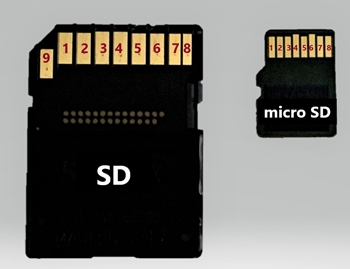
\includegraphics[height=6cm]{BilderExt/microchip_sdcards.jpg}
        \caption{Pinnummerierung SD-Karten\cite{microchip_sd}}
        \label{fig:sd_num}
    \end{figure}


\subsubsection{SPI-Peripherie des STM32G431}
\begin{figure}[H]
    \centering
    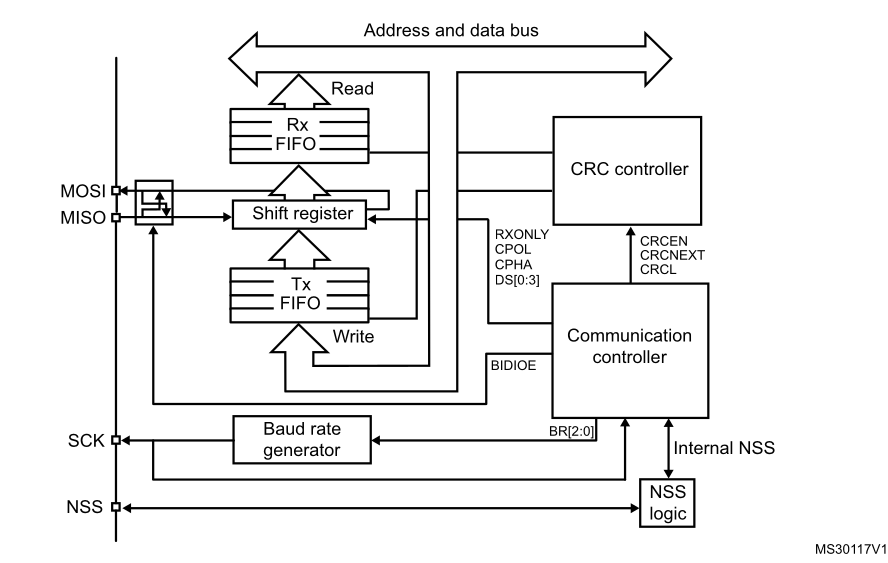
\includegraphics[width=0.7\linewidth]{BilderExt/st-blockdiagram.png}
    \caption{Blockdiagramm f"ur die SPI-Peripherie des STMG431 \cite{st3}}
    \label{fig:stblock}
\end{figure}
\fig{fig:stblock} zeigt das Blockdiagramm f"ur die SPI-Peripherie der STM32G4-Serie.
Der relevanteste Teil ist das Shiftregister. Das oberste Bit des Shiftregisters wird auf MOSI ausgegeben.
Gleichzeitig wird das Bit auf MISO eingelesen. Es liegt in der verwendeten Konfiguration immer eine Full-Duplex "Ubertragung vor.
Um Daten über MISO zu empfangen, muss der Master eine Übertragung initiieren und entsprechend Taktzyklen erzeugen. 
Dabei werden gleichzeitig Daten über MOSI übertragen.\\
Der Baudratencontroller ist f"ur die SCLK und somit f"ur die "Ubertragungsgeschwindigkeit zust"andig.
Er nutzt den APB-Bus-Takt und teilt ihn, falls im BR-Register konfiguriert, durch einen Prescaler. \\
F"ur den Zweck der SD-Karten-Kommunikation wurde die SPI-Peripherie als Master konfiguriert, mit 
einem frei w"ahlbaren, softwareseitig zuschaltbaren NSS-Pin (Chip Select).


\begin{listing}[H]
    \begin{minted}[
        frame=lines,      % Rahmenlinien oben und unten
        framesep=2mm,     % Abstand zum Rahmen
        baselinestretch=1.2,
        bgcolor=lightgray!20, % Hintergrundfarbe
        fontsize=\footnotesize,
        linenos           % Zeilennummern aktivieren
    ]{cpp}
template<uintptr_t PortBase, uint32_t Pin>
struct ChipSelect {
private:
    static inline GPIO_TypeDef* const port = reinterpret_cast<GPIO_TypeDef*>(PortBase);
public:
    ChipSelect() {
        port->BSRR = (1U << (Pin + 16));
    }

    ~ChipSelect() {
        port->BSRR = (1U << Pin);
    }
};
    \end{minted}
\caption{Auszug aus der \texttt{src/sdcarddriver.hpp}}
\label{listing:chipselect}
\end{listing}


Der Quellcode \ref{listing:chipselect} zeigt die St"arke von C++ im Gegensatz zu C in diesem Kontext.
Der NSS-Pin muss am Anfang der meisten SD-Funktionen wie \cpp{SD_ReadBlock}
oder \cpp{SD_SendCmd} auf Low konfiguriert werden und beim Verlassen der Funktion wieder auf High.
Mit \cpp{ChipSelect<GPIOA_BASE, 8> chipselect_tmp;} w"urde ein Objekt erzeugt werden. Beim Konstruieren, also dem Erzeugen
des Objektes, w"urde der Konstruktor Pin 8 von GPIOA auf Low setzen, und beim Verlassen der Funktion w"urde der Destruktor aufgerufen
werden und den Pin wieder auf High setzen. In C m"ussten alle Stellen gefunden werden, bei denen die Funktion verlassen wird,
oder es m"ussten Laufzeitkosten in Kauf genommen werden mit dem Aufruf einer Helferfunktion.
Die Informationen, welche GPIO-Ports mit welchen Pins benutzt werden sollen, stehen zur Compilezeit fest; der verwendete
Cast ist \cpp{static inline const},
sodass ein guter C++-Compiler die gesamte Klasse vollständig auf zwei direkte Registerzugriffe reduzieren kann.


\subsubsection{SPI Treiber}
Die Quelldatei \texttt{/src/spidriver.hpp} kapselt die hardwarenahe Konfiguration und Kommunikation über die SPI-Peripherie des STM32G431.
Die Initialisierung konfiguriert den jeweiligen SPI-Controller als Master mit softwaregesteuertem NSS
und einer Datenbreite von acht Bit. Die Methode \cpp{static uint8_t Transfer(uint8_t data)} kapselt schließlich das Senden und Empfangen eines Bytes 
und übernimmt dabei die notwendige Synchronisation mit den Statusflags der SPI-Peripherie.
Zus"atzlich kann der verwendete Baudratenteiler über die Methode \cpp{static void SetHighSpeed(SpiDiv div)} verwendet werden,
um zwischen einer Initialisierung mit niedriger und einer sp"ateren Kommunikation mit höherer "Ubertragungsgeschwindigkeit zu wechseln.
Der maximale SPI-Clock kann dabei auf maximal die H"alfte des Systemtaktes festgelegt werden: Da in dem Fall der vorliegenden Arbeit
kein gesonderter Takt in den RCC-Registern konfiguriert wurde, 
arbeitet der Mikrocontroller mit dem internen Takt des RC-Oszillators von 16\,MHz, sodass ein SPI-Takt von 8\,MHz m"oglich ist.

\subsection{Initialisierung der SD-Karte in den SPI-Modus}

\begin{figure}[H]
    \centering
    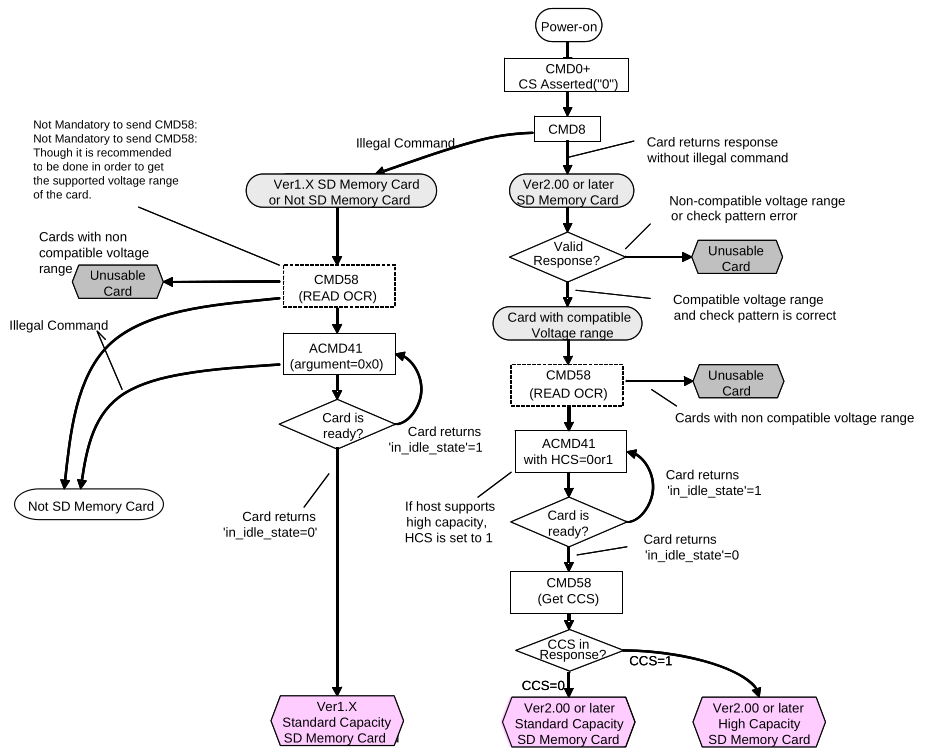
\includegraphics[height=12cm]{BilderExt/sd_spec_SPIINIT.png}
    \caption{Initialisierung der SD-Karte in den SPI-Modus \cite{sd_spec}}
    \label{fig:sd_spiinit}
\end{figure}

\fig{fig:sd_spiinit} zeigt den vollst"andigen Initialisierungsprozess als Flussdiagramm aus der SD-Spezifikation.
Die Initialisierung und Treiberfunktionen finden sich in der Datei \texttt{src/sdcarddriver.hpp}. Die praktische Implementierung der Initialisierung 
ist etwas verk"urzt worden; wie auf der Abbildung zu sehen ist, ist CMD58 nur notwendig, wenn Interesse an den unterst"utzten Spannungsbereichen
der SD-Karte besteht. 3,3 V Betriebsspannung ist aber f"ur praktisch jede auf dem Markt gebr"auchliche SD-Karte zul"assig.
Zumal die Spezifikation den Nutzer hier vor ein klares Henne-Ei-Problem stellt: Ohne eine geeignete Spannungsversorgung l"asst sich 
der unterst"utzte Spannungsversorgungsbereich der Karte nicht auslesen.\\
Weiterhin unterschl"agt die Abbildung die Tatsache, dass f"ur die Benutzung von ACMD41 zun"achst einmal CMD55 gesendet
werden muss. Diese Information muss aus einem anderen Teil der Dokumentation entnommen werden. 

\begin{listing}[H]
    \begin{minted}[
        frame=lines,      % Rahmenlinien oben und unten
        framesep=2mm,     % Abstand zum Rahmen
        baselinestretch=1.2,
        bgcolor=lightgray!20, % Hintergrundfarbe
        fontsize=\footnotesize,
        linenos           % Zeilennummern aktivieren
    ]{cpp}
    template<typename Config>
    uint8_t SD_InitSPI()
    {
    (...)
    ChipSelect<Config::PortBase, Config::Pin> chipselect_tmp;
    // CMD0
    //Give it some tries, does not work the first time, because card is busy...
    for (int i = 0; i < 20; ++i)
    {
        cmd0_resp = SD_SendCmd<Config>(0, 0, 0x95, nullptr, 0);

        if (cmd0_resp == 0x01)
            break;
    }

    if (cmd0_resp != 0x01)
    return SD_INIT_ERROR_CMD0;

    // CMD8
    SD_SendCmd<Config>(8, 0x000001AA, 0x87, cmd8_resp, 4);

    if (cmd8_resp[0] != 0x01 || cmd8_resp[4] != 0xAA)
        return SD_INIT_ERROR_CMD8;
    (...)
    }
    \end{minted}
    \caption{Auszug aus der Funktion \cpp{SD_InitSPI}}
    \label{listing:sdcardinit}
\end{listing}

\coderef{listing:sdcardinit} zeigt einen Auszug aus der Initialisierungsfunktion,
\coderef{listing:sdcardsendcmd} beschreibt die verwendete \cpp{SD_SendCmd} Funktion.
\cpp{SD_SendCmd} nutzt den zugrunde liegenden SPI-Treiber, um auf der im Templateparameter Config
spezifizierten Peripherie die korrekten Daten "uber
die bereits implementierte \\
\cpp{Transfer(uint8_t Data)} Funktion zu senden.
Die Daten f"ur die Peripherien k"onnen in der Datei \\
\texttt{src/init\_conf.hpp} konfiguriert werden.
F"ur die vorliegende Arbeit und Platine sind diese nat"urlich fix, allerdings l"asst der 
STM32G431 einiges an Spielraum zu, was variable Peripheriekonfiguration angeht.\\
Wichtig ist hierbei, dass CMD0 und CMD8 zun"achst korrekte CRC-Werte f"ur ihre Befehle
ben"otigen. Das SD-Protokoll spezifiziert hier f"ur den SPI-Modus etwas anderes als
f"ur den SD-Modus: Im normalen SD-Modus wird bei grunds"atzlich jedem CMD die Pr"ufsumme
gepr"uft und muss daher mitgesendet werden. Im SPI-Modus ist diese Pr"ufsummenberechnung
grunds"atzlich deaktiviert und kann optional mit CMD59 aktiviert werden. Dies gilt
aber nicht f"ur CMD0 und CMD8; diese Befehle brauchen immer einen korrekten CRC7-Wert.
\begin{listing}[H]
    \begin{minted}[
        frame=lines,      % Rahmenlinien oben und unten
        framesep=2mm,     % Abstand zum Rahmen
        baselinestretch=1.2,
        bgcolor=lightgray!20, % Hintergrundfarbe
        fontsize=\footnotesize,
        linenos           % Zeilennummern aktivieren
    ]{cpp}
    template<typename Config>
    uint8_t SD_SendCmd(uint8_t cmd, uint32_t arg, uint8_t crc, uint8_t *response_buf, uint8_t extra_bytes)
    {

    uint8_t r1;
    uint16_t timeout = 0;

    // send cmd
    SpiDriver<Config::SpiBase>::Transfer(cmd | 0x40);
    
    // 4 byte argument
    SpiDriver<Config::SpiBase>::Transfer((uint8_t)(arg >> 24));
    SpiDriver<Config::SpiBase>::Transfer((uint8_t)(arg >> 16));
    SpiDriver<Config::SpiBase>::Transfer((uint8_t)(arg >> 8));
    SpiDriver<Config::SpiBase>::Transfer((uint8_t)arg);
    
    // 1 byte CRC (SPI-Mode ignores it, but still needed even then... Needed for CMD0 and CMD8 though!)
    SpiDriver<Config::SpiBase>::Transfer(crc);
    (...)
    }
    \end{minted}
\caption{Auszug aus der Funktion \cpp{SD_SendCmd}}
\label{listing:sdcardsendcmd}
\end{listing}

\coderef{listing:sdcardsendcmd} verdeutlicht, wie das Senden von einzelnen SD-Befehlen "uber die SPI-Peripherie
prinzipiell funktioniert. Tats"achlich wurde die Funktion \cpp{SD_SendCmd} selten verwendet, da nach dem 
Senden des 4-Byte Arguments meistens noch f"ur die konkreten SD-Befehle spezifische Abl"aufe folgen. 

%Das ist f"ur die Funktion des Treibers wichtig, da dieser in der Initialisierungsphase

\subsection{Lese- und Schreiboperationen}
%Sektor => physisch hardware kleinste Einheit
%Block => logisch Software kleinste Einheit
\subsubsection{Begriffskl"arung Sektor, Block, Cluster, Page}
F"ur die weitere Arbeit m"ussen hier im Zusammenhang mit Blockspeicher 
zun"achst h"aufig verwendete Begriffe gekl"art werden:
Ein Sektor bezeichnet die kleinste physikalisch adressierbare Speichereinheit eines Datenträgers.
Ein Block bezeichnet dagegen die kleinste logische Speichereinheit, 
die von einem Betriebssystem oder Dateisystem adressiert wird. Ein Block kann also gr"o"ser
sein als ein Sektor, aber nicht anders herum.\\
Ein Cluster ist genau dasselbe wie ein Block, taucht aber im Zusammenhang mit dem
FAT-Dateisystem auf, wohingegen der Block in der Unixwelt gel"aufiger ist.\\
Im Zusammenhang mit Flashspeicher wird die Page als kleinste programmierbare Einheit beschrieben,
wohingegen der Erase Block die kleinste löschbare Einheit beschreibt.\\
Leider werden in Spezifikationen und Literatur die Begrifflichkeiten nicht eindeutig verwendet.
So spricht man im Zusammenhang von SD-Karten in aller Regel von Bl"ocken, die beschrieben werden,
obwohl der Begriff des Sektors hier manchmal synonym verwendet wird. 
Hier wird im Folgenden von Bl"ocken die Rede sein, womit aber die kleinste von 
der SD-Karte adressierbare Einheit gemeint ist.\\

\subsubsection{SD-Karte als Blockspeicher}
Die essenzielle Funktionalit"at der SD-Karte ist das Lesen und Schreiben von Bl"ocken.
F"ur die verwendeten Dateisysteme ist die SD-Karte als Blockspeicher
abstrahiert worden. Das Dateisystem \enquote{wei"s} gar nicht, dass es eine
SD-Karte verwendet, sondern ihm werden lediglich Funktionen zur Verf"ugung
gestellt, mit denen es einzelne oder mehrere Bl"ocke schreiben und lesen kann.\\
Die Funktionen des SD-Treibers finden sich in der Datei \texttt{src/sdcarddriver.hpp}.


\subsubsection{Lesefunktionen}
F"ur das blockweise Lesen eines Blocks wurde die Funktion 
\cpp{uint8_t SD_ReadBlock(uint32_t block_addr, uint8_t *buffer)} implementiert.
Die Funktion \\
\cpp{uint8_t SD_ReadBlocks(uint32_t block_addr, uint32_t block_count, uint8_t *buffer)}
hingegen implementiert das Lesen von mehreren Bl"ocken. Das Argument \cpp{uint32_t block_count}
gibt dabei an, wie viele Bl"ocke hintereinander gelesen werden sollen, wohingegen
\cpp{uint32_t block_addr} den Startblock angibt, angefangen bei Block 0.
Da das Feld 32-bit gro"s ist, lassen sich damit genau 
$
\frac{2^{32} \cdot 512}{1024^4} = 2 \,\text{TB}
$
an Daten adressieren. Dies gilt f"ur den modernen SDHC/SDXC-Kartenstandard und somit 
f"ur den ansoluten Gro"steil aller heutigen SD-Karten. 
Der "altere SDSC-Standard hat auf eine Byteadressierung gesetzt und hat somit 
ein Speicherlimit von 2\,GB. Vereinzelt braucht es allerdings SDSC-Karten noch f"ur alte
Hardware aus den fr"uhen 2000er Jahren, die den neuen Standard nicht implementiert hat.

\begin{figure}[H]
    \centering
    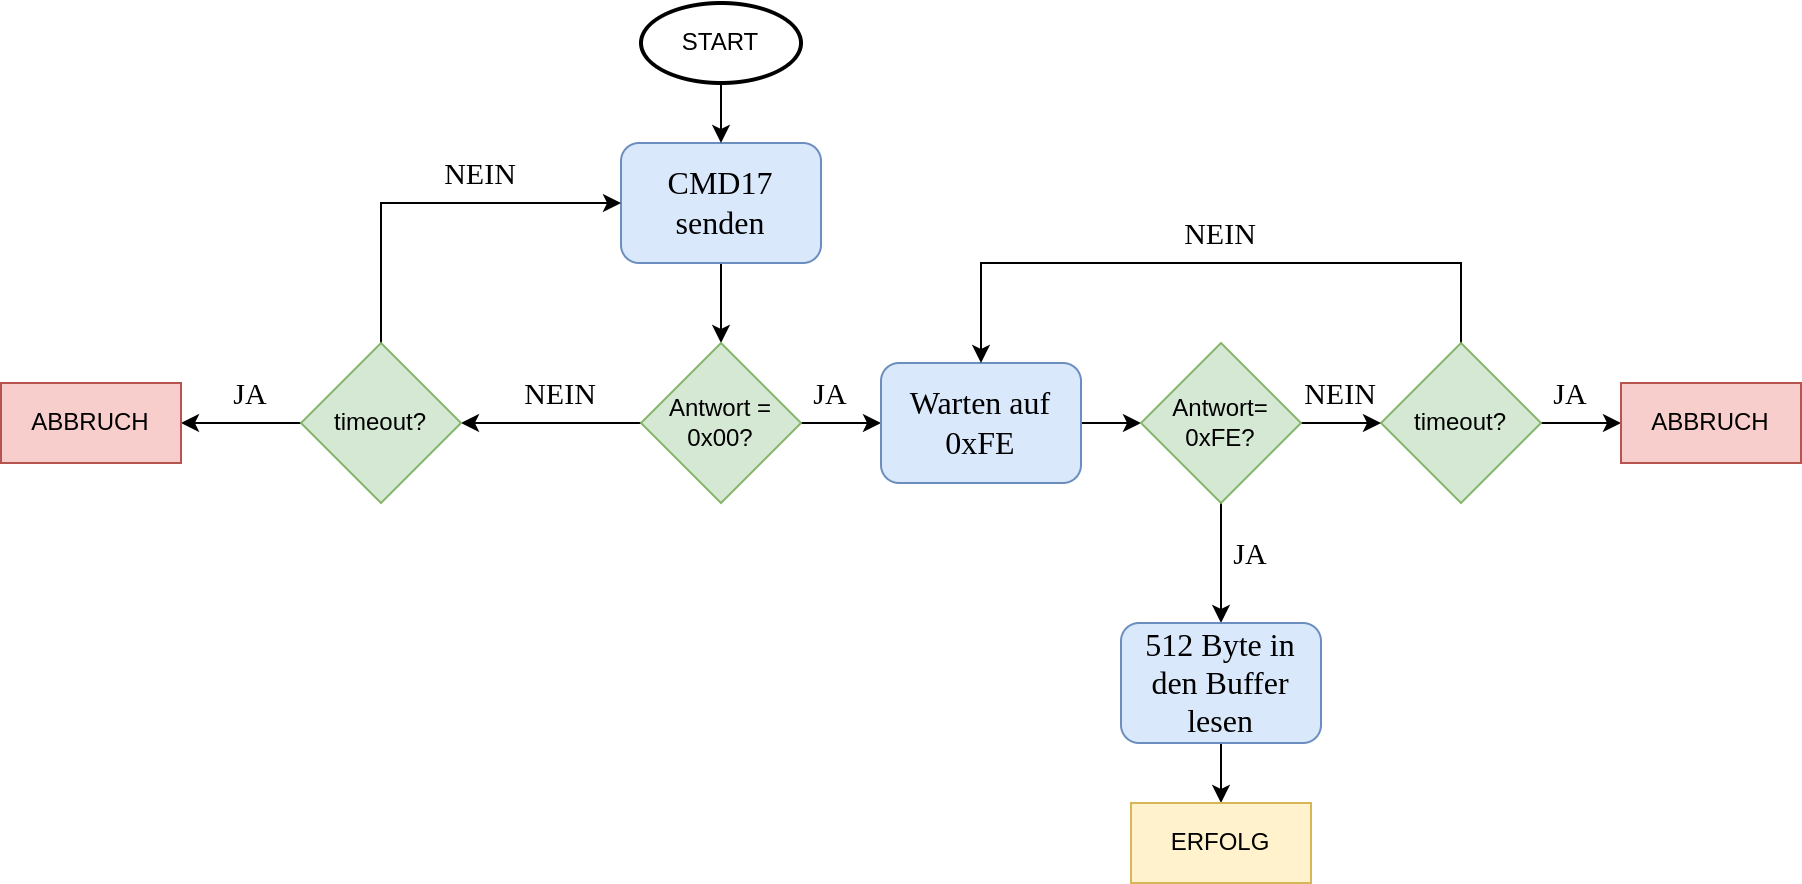
\includegraphics[width=\textwidth]{Bilder_Diagramme/CMD17.png}
    \caption{Flussdiagramm des prinzipiellen Ablaufs der \cpp{SD_ReadBlock}-Funktion}
    \label{fig:sd_flowchartcmd17}
\end{figure}

\fig{fig:sd_flowchartcmd17} zeigt ein Flussdiagramm f"ur die \cpp{SD_ReadBlock}-Funktion.
CMD17 entspricht dem Befehl \enquote{Read Single Block} aus der SD-Spezifikation und
kann nach der Initialisierung der SD-Karte in den SPI-Modus gesendet werden.
Wenn die Karte nach dem Empfang des CMD17 bereit ist, so sendet sie ein \texttt{0x00}-Byte zur"uck und im
Anschluss ein \texttt{0xFE}-Byte. Nach dem \texttt{0xFE}-Byte folgt dann der angeforderte Block 
bestehend aus 512 Bytes an Daten, die in einen Buffer eingelesen werden k"onnen. \\
An zahlreichen Stellen wird durch
einen Timeout sichergestellt, dass die Funktion bei Fehlschlag nicht den gesamten
Programmfluss blockiert. Die SD-Spezifikation gibt hier keine Vorgaben, also wurden
Werte bis zur Bew"ahrung getestet.\\


\begin{listing}[H]
    \begin{minted}[
        frame=lines,      % Rahmenlinien oben und unten
        framesep=2mm,     % Abstand zum Rahmen
        baselinestretch=1.2,
        bgcolor=lightgray!20, % Hintergrundfarbe
        fontsize=\footnotesize,
        linenos           % Zeilennummern aktivieren
    ]{cpp}
    // wait for start 0xFE
    start_time = TIM2->CNT;
    do {
        r1 = SpiDriver<Config::SpiBase>::Transfer(0xFF);
    } while ((r1 != 0xFE) && ((TIM2->CNT - start_time) < T_OUT2_US));

    if (r1 != 0xFE) {
        //SD_CS_DESELECT();
        return 0x02; // timeout-error waiting for 0xFE
    }

    // read 512 byte blockdata
    for (uint16_t i = 0; i < 512; i++) {
        buffer[i] = SpiDriver<Config::SpiBase>::Transfer(0xFF);
    }

    \end{minted}
\caption{Auszug aus der Funktion \cpp{SD_ReadBlock}}
\label{listing:lesefunktionen}
\end{listing}

\coderef{listing:lesefunktionen} zeigt beispielhaft einen Auszug der Funktion \cpp{SD_ReadBlock}, 
der auf das \texttt{0xFE-Byte} wartet und danach 512 Bytes empf"angt. Da die SPI-Peripherie
immer gleichzeitig sendet und empf"angt, m"ussen f"ur den Empfang von Bytes willk"urliche 
Daten gesendet werden. Ebenfalls zeigt der Auszug, wie mittels eines Hardwaretimers der Timeout 
implementiert wurde. \\
Die Funktion \cpp{SD_ReadBlocks} ist die etwas komplexere Version, die f"ur
das Lesen von multiplen Bl"ocken genutzt werden kann. Dies hat den Vorteil,
dass es den Overhead im Vergleich mit der Payload minimiert: W"ahrend bei der 
\cpp{SD_ReadBlock}-Funktion f"ur alle 512 Bytes einmal CMD17 gesendet 
werden muss, zuz"uglich aller potenziellen Wartezeiten im SD-Controller, so reicht
ein CMD18-Befehl f"ur beliebig viele 512 Byte Bl"ocke.\\
Prinzipiell ist der Programmablauf "ahnlich: Zun"achst muss CMD18 gesendet werden.
Das entspricht dem Befehl \enquote{Read Multiple Block} aus der Spezifikation.
Nach dem \texttt{0xFE}-Byte folgen aber so lange Bytes, bis ein CMD12 (\enquote{Stop Transmission})
den Datenfluss unterbricht. \\
Es sollte beachtet werden, dass die Buffergr"o"se f"ur \cpp{SD_ReadBlocks} ein Vielfaches 
von 512 Byte sein muss, wobei der Faktor dem Argument \texttt{block\_count} gleicht. 


\subsubsection{Schreibfunktionen}
F"ur das blockweise Schreiben eines einzelnen 512 Byte Blocks stellt
der SD-Treiber die Funktion
\cpp{uint8_t SD_WriteBlock(uint32_t block_addr, const uint8_t *buffer)}
zur Verf"ugung.
F"ur das Schreiben von multiplen Bl"ocken hintereinander existiert die Funktion
\cpp{uint8_t SD_WriteBlocks(uint32_t block_addr, uint32_t block_count, const uint8_t *buffer)}.
Die Argumente verhalten sich analog zu denen der lesenden Funktionen.


\begin{figure}[H]
    \centering
    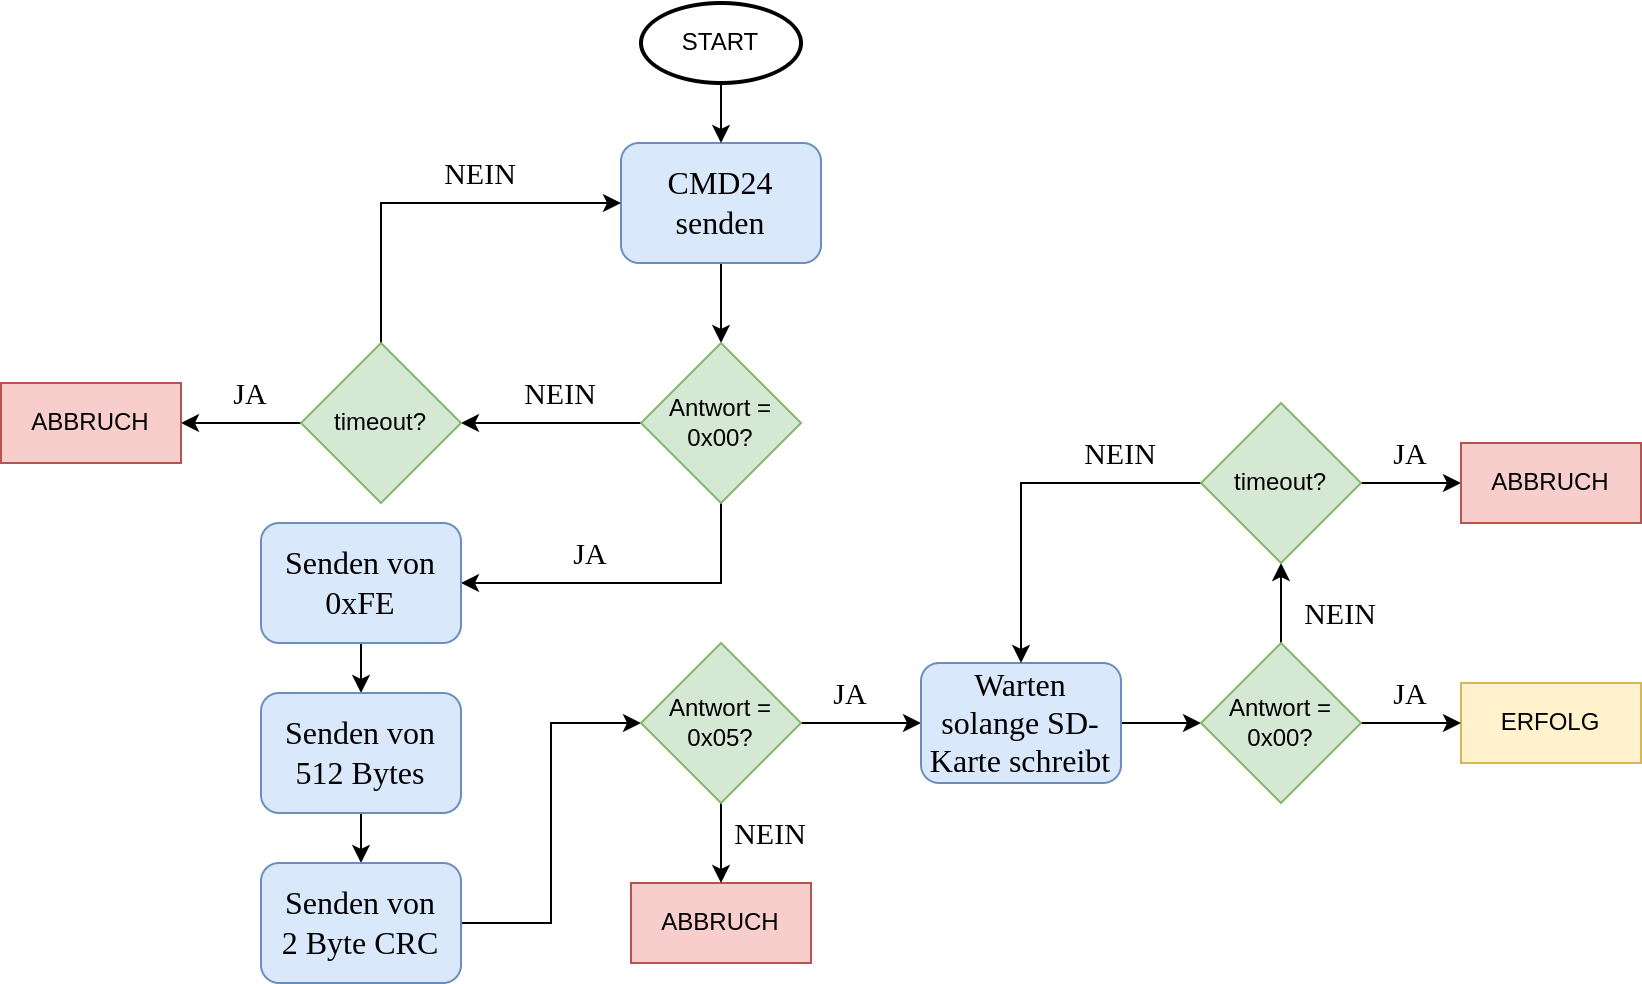
\includegraphics[width=\textwidth]{Bilder_Diagramme/CMD24.png}
    \caption{Flussdiagramm des prinzipiellen Ablaufs der \cpp{SD_WriteBlock}-Funktion}
    \label{fig:sd_flowchartcmd24}
\end{figure}

\fig{fig:sd_flowchartcmd24} zeigt den prinzipiellen Programmfluss f"ur den 
SD-Befehl CMD24 \enquote{Write Single Block}. Zun"achst wird wie immer
der entsprechende Befehl, hier CMD24, gesendet. Bei erfolgreicher
Antwort wird mit dem Startbyte \texttt{0xFE} der Beginn der "Ubertragung
signalisiert. Dann folgen 512 Bytes an zu schreibenden Daten und es wird
mit 2 Bytes CRC abgeschlossen. Wichtig ist hier zu beachten, dass die
CRC in jedem Fall gesendet werden muss, auch wenn die entsprechende
"Uberpr"ufung ausgeschaltet ist: In dem Falle kann aber auf die 
Berechnung einer echten CRC verzichtet werden und es k"onnen stattdessen beliebige
2 Bytes gesendet werden. Im n"achsten Schritt muss die SD-Karte mit einem
\texttt{0x05} antworten, falls die CRC-"Uberpr"ufung erfolgreich war. \\
Die Funktion kann erfolgreich verlassen werden, wenn die SD-Karte im Anschluss mit 
einem \texttt{0x00} signalisiert, dass alle Daten erfolgreich im Flash abgelegt werden konnten.\\
Der SD-Befehl CMD25 f"ur das Schreiben von mehreren Bl"ocken "ahnelt vom Ablauf her 
sehr CMD24. Statt dem \texttt{0xFE}-Byte kommt hier ein \texttt{0xFC}-Byte als Startbyte
zum Einsatz. Es wird weiterhin in 512 Byte Abschnitten gearbeitet: Zun"achst werden Startbyte + 512 Byte Daten + 2 Byte CRC geschrieben,
dann sendet die SD-Karte ein Statusbyte, in dem sie die erhaltene Information akzeptiert. 
Im Anschluss wird darauf gewartet, dass die SD-Karte den Block tats"achlich geschrieben hat.
Dieser Ablauf erfolgt f"ur alle zu schreibenden Bl"ocke in einer Schleife. 
Am Ende folgt dann statt dem \texttt{0xFC}-Startbyte f"ur einen neuen Block ein \texttt{0xFD}-Stopbyte,
welches den Schreibvorgang beendet.



\subsubsection{Statusfunktionen}
Zu guter Letzt braucht es f"ur eine Implementation von Dateisystemen als Information zumindest
die Speicherkapazit"at der SD-Karte. Die Rohinformation l"asst sich mit   
\cpp{uint8_t SD_GetCSD(uint8_t *buffer, const uint8_t BUF_SIZE)}
abrufen. Diese Funktion nutzt den SD-Befehl CMD9 \enquote{Send CSD}.


\begin{listing}[H]
    \begin{minted}[
        frame=lines,      % Rahmenlinien oben und unten
        framesep=2mm,     % Abstand zum Rahmen
        baselinestretch=1.2,
        bgcolor=lightgray!20, % Hintergrundfarbe
        fontsize=\footnotesize,
        linenos           % Zeilennummern aktivieren
    ]{cpp}
    // wait for start 0xFE
    start_time = TIM2->CNT;
    do {
        r1 = SpiDriver<Config::SpiBase>::Transfer(0xFF);
    } while ((r1 != 0xFE) && ((TIM2->CNT - start_time) < T_OUT2_US));

    if (r1 != 0xFE) {
        //SD_CS_DESELECT();
        return SD_CSD_ERROR_DATATRANS; // timeout-error waiting for 0xFE
    }

    // read 16 byte CSD register
    constexpr uint8_t CSD_SIZE = 16;
    for (uint8_t i = 0; i < CSD_SIZE; i++) {
        buffer[i] = SpiDriver<Config::SpiBase>::Transfer(0xFF);
    }
    }
    \end{minted}
\caption{Auszug aus der Funktion \cpp{SD_GetCSD}}
\label{listing:statusfunktionen}
\end{listing}
\coderef{listing:statusfunktionen} zeigt den wichtigsten Teil der \cpp{SD_GetCSD}-Funktion.
Diese arbeitet im Prinzip genauso wie die \cpp{SD_ReadBlock}-Funktion, mit der Ausnahme, 
dass sie eine von der SD-Karte fixe 16 Byte Sequenz erh"alt, die sogenannte CSD (Card Specific Data).
Diese enth"alt eine Vielzahl an Informationen, wie beispielsweise die maximale
"Ubertragungsgeschwindigkeit der SD-Karte pro Datenleitung. Die genaue Bedeutung der Informationen
unterscheidet sich allerdings einmal wieder je nachdem, ob eine alte SDSC-Karte (CSD V1.0) oder
eine moderne SDHC/SDXC-Karte (CSD V2.0) vorliegt. Alle Details befinden sich in der SD-Spezifikation.
Als Hinweis sei hier aber noch erw"ahnt, dass in der CSD V2.0 zwar zum Beispiel das Feld
\enquote{erase sector size} tabellarisch auftaucht und genau so benannt wird, es aber nicht f"ur die Gr"o"se
des L"oschblocks steht. Tats"achlich wird das Feld in CSD V2.0 schlichtweg nicht genutzt, was erst in 
der erweiterten Beschreibung des Feldes erl"autert wird. 
Die SD-Spezifikation hat das Feld dennoch nicht umbenannt. \\
Die Funktion
\cpp{uint8_t parse_csd(const uint8_t* rawcsd, Csd_Common* csd)}
extrahiert aus der Vielzahl von Informationen lediglich die Kartengr"o"se,
da dies im Folgenden die einzig relevante Information darstellt. 



\section{Dateisysteme}
\subsection{Einleitung}
Eine umfassende Einführung in die Grundlagen von Dateisystemen wird 
von Tanenbaum und Bos in ihrem Standardwerk \textit{Modern Operating Systems} bereitgestellt \cite[S.~263 ff.]{tanenbaum2015}.
Laut den Autoren werden drei essenzielle Anforderungen an die Langzeitspeicherung von Daten gestellt:
\begin{enumerate}
    \item Es muss möglich sein, eine sehr gro"se Menge an Informationen zu speichern.
    \item Die Informationen müssen das Beenden des Prozesses, der sie verwendet, überdauern.
    \item Mehrere Prozesse müssen gleichzeitig auf die Informationen zugreifen können.
\end{enumerate}

Tanenbaum und Bos nutzen in ihrem Buch den Begriff des Prozesses zur Ressourcenverwaltung und -abstraktion, 
w"ahrend diese Notwendigkeit in der vorliegenden Arbeit entf"allt, 
da das Programm direkte Kontrolle über die gesamte Hardware des Mikrocontrollers besitzt.
Im Prinzip k"onnte das Problem, eine gro"se Menge an Information zu speichern bereits mit zwei Operationen
l"osen:
\begin{enumerate}
    \item Einen w"ahlbaren Block lesen
    \item Einen w"ahlbaren Block schreiben
\end{enumerate}

Das sind exakt die Operationen, die in dem vorherigen Kapitel \ref{sec:spi} f"ur die SD-Karte implementiert wurden.
In der Praxis sind diese zwei Operationen allerdings zu primitiv, um Daten effektiv zu verwalten.
Tanenbaum und Bos stellen beispielhaft folgende Fragen:
\begin{itemize}
    \item Wie findet man eine bestimmte Information
    \item Wie verhindert man (auf Mehrbenutzersystemen), dass ein Benutzer die Daten eines anderen ausliest?
    \item Woher wei"s man, welche Bl"ocke frei sind?
\end{itemize}

F"ur diese und viele andere praktische Probleme hilft das Konzept der Datei.
Die Datei ist etymologisch ein Neologismus aus Daten und Kartei.
Im Kontext moderner Betriebssysteme definieren Tanenbaum und Bos Dateien als 
logische Einheiten von Information, die von Prozessen erzeugt werden und diese "uberdauern.
Eine Datei soll erst gel"oscht werden, wenn ein Besitzer dies explizit veranlasst \cite{tanenbaum2015}.\\
Wie Dateien strukturiert, benannt, aufgerufen, genutzt, geschützt, implementiert und verwaltet werden ist Sache
des Dateisystems. Ein Dateisystem l"ost (je nach Funktionsumfang) viele der oben gestellten Anforderungen.
Aus Sicht des Nutzers ist der wichtigste Aspekt eines Dateisystems,
wie es sich darstellt: Was eine Datei ausmacht, wie Dateien benannt und geschützt werden, 
welche Operationen auf Dateien erlaubt sind. Die Details darüber, ob verkettete Listen oder Bitmaps verwendet werden, 
um den freien Speicherplatz zu verwalten, oder wie viele Sektoren ein logischer Festplattenblock enthält, sind für den Nutzer von keinem Interesse,
obwohl sie für die Entwickler des Dateisystems von großer Bedeutung sind \cite{tanenbaum2015}.
Zusammenfassend l"asst sich sagen, dass ein Dateisystem eine f"ur den Anwendungszweck geeignete Struktur in einen rohen Speicherbereich bringt.
W"ahrend Tanenbaum und Bos den Schwerpunkt auf Dateisystemen f"ur Betriebssysteme legen, 
was sicherlich der "ubliche Anwendungsbereich ist, geht es in dieser Arbeit um die Verwendung
von Dateisystemen in eingebetteten Systemen, bzw. konkret auf einem STM32G431 und um deren Vor- und Nachteile hinsichtlich der Nutzung.

\subsection{Layout eines Dateisystem}
W"ahrend das Design eines Dateisystems grunds"atzlich frei entschieden werden kann,
folgt die Struktur meist einem "ahnlichen Muster, sodass die Kl"arung einiger "ublicher Begriffe
n"otig ist.
\begin{figure}[H]
    \centering
    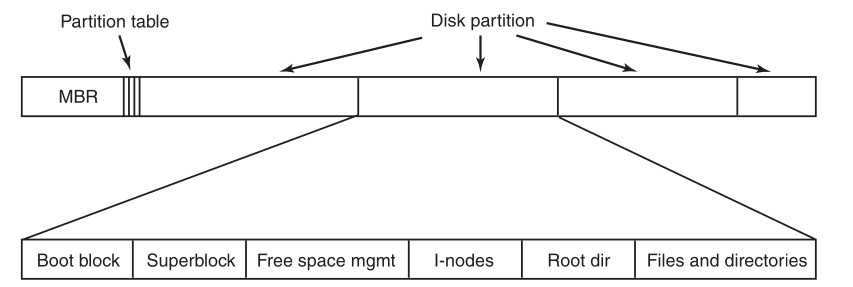
\includegraphics[width=1\linewidth]{Bilder/TAN_Filesystem.png}
    \caption{Ein m"ogliches Dateisystemlayout \cite[S. 282]{tanenbaum2015}}
    \label{fig:fslayout}
\end{figure}
\fig{fig:fslayout} zeigt ein m"ogliches Layout eines Dateisystems nach Tanenbaum und Bos \cite[S.~282]{tanenbaum2015}.
Der erste Sektor eines Speichermediums wird reserviert f"ur den MBR (Master Boot Record) und wird "ublicherweise
zum Starten eines Computers verwendet. Das Ende des MBR enth"alt die Partitionstabelle, in welcher eine
der Partitionen als aktiv markiert ist. Ein physisches Medium kann mehrere Partitionen und somit mehrere Dateisysteme 
beinhalten. Wenn der Computer gebootet wird, dann stellt ein Programm fest, welche Partition
aktiv ist und f"uhrt die Anweisungen in dem \enquote{Boot block} aus. "Ublicherweise folgt darauf Superblock, in dem
wichtige Informationen "uber das Dateisystem stehen wie der Typ des Dateisystems oder die Anzahl der vorhandenen Bl"ocke.
Im Anschluss folgen typischerweise Informationen über die freien Blöcke des Dateisystems, 
die beispielsweise in Form einer Zeigerliste organisiert sind. 
Darauf folgen die sogenannten I-Nodes, ein Array von Datenstrukturen, das für jede Datei existiert
und alle relevanten Datei-Metadaten enthält. 
Danach schließt sich das Wurzelverzeichnis (Root Directory) an, 
welches die Wurzel der gesamten Dateisystemstruktur bildet. 
Der verbleibende Speicherplatz des Datenträgers steht schließlich für alle weiteren Verzeichnisse
und die eigentlichen Dateien zur Verfügung\cite[S. 282]{tanenbaum2015}.\\
W"ahrend Felder wie der MBR von praktisch allen Dateisystemen beachtet werden,
unterscheidet sich das Layout teilweise doch deutlich von dem vorgestellten, theoretischen
Entwurf nach Tanenbaum und Bos.\\


Die Autoren des littlefs-Dateisystems kategorisieren auf ihrer
\href{https://github.com/littlefs-project/littlefs/blob/master/DESIGN.md}{GitHub Seite} 
in der Datei \enquote{DESIGN.md}
Dateisysteme sehr "ubersichtlich in vier Gruppen \cite{littlefs}:

\subsubsection{Nicht-resiliente, blockbasierte Dateisysteme}
Bekannte Vertreter sind hier FAT f"ur Microsoftsysteme und ext2 f"ur Linux-Betriebssysteme.
Diese grundlegenden Systeme führen Aktualisierungen direkt an Ort und Stelle
und ohne Absicherungsmechanismen durch. Dadurch sind sie bei pl"otzlichen Stromausf"allen 
sehr anf"allig für Datenkorruption. Im Zusammenhang mit Flashspeicher ist ein weiterer Nachteil,
dass derselbe Block somit mehrfach beschrieben wird und es zur einer schnellen Abnutzung des Speichers kommt.
Vorteile sind jedoch, dass diese Dateisysteme meistens 
sehr schnell und klein sind, sowie einfach in der Implementation.

\subsubsection{Logging-Dateisysteme}
Reine Logging-Dateisysteme sind heutzutage selten in Benutzung. 
Vertreter hiervon hei"sen JFFS, YAFFS, SPIFFS.
Anstatt Daten direkt zu "uberschreiben, 
behandeln diese Systeme das Speichermedium als fortlaufendes, 
anhängendes Protokoll. Hier ist der Speicherort nicht an einen bestimmten
Speicherblock gebunden.
Mit einer Pr"ufsumme l"asst sich ein Stromausfall leicht erkennen
und auf den vorherigen Zustand zur"ucksetzen, indem man fehlgeschlagene Anhänge einfach ignoriert.
Au"serdem sorgt die zyklische Natur dafür, dass Logging-Dateisysteme den Verschleiß
perfekt über den Speicher verteilen.
Dies minimiert die Löschzyklen auf Flashspeichern 
und garantiert eine hohe Ausfallsicherheit.
Nachteile sind die verh"altnism"a"sig hohen Laufzeitkosten (h"aufig O($n^2$)) und der hohe RAM-Verbrauch,
was sie f"ur Embeddedanwendungen eher ungeeignet macht.
\subsubsection{Journaling-Dateisysteme}
Bekannte und moderne Vertreter sind hier ext3, ext4 f"ur Linuxbetriebssysteme oder
NTFS f"ur Windows. Diese Systeme schlagen die Br"ucke zwischen blockbasierten und logging-strukturierten Designs
und haben gro"se Vorteile, was die Korruption von Daten im Falle eines Stromausfalls angeht.
Der Prozess findet im Falle von ext4 dabei konzeptionell vereinfacht wie folgt statt:
Zunächst werden die für die "Anderung wichtigen Informationen in das sogenannte Journal des Dateisystems geschrieben.
Sobald diese Informationen vollst"andig auf dem Datentr"ager gespeichert wurden, 
wird die Transaktion durch einen Commit-Eintrag im Journal bestätigt.
Anschließend werden die Änderungen an ihre endgültige Position im Dateisystem geschrieben.
Nach erfolgreicher Übertragung wird der Commit-Eintrag nicht mehr benötigt und kann entfernt werden.
Kommt es während dieses Vorgangs zu einem Systemabsturz,
kann das Dateisystem beim nächsten Start das Journal auswerten. 
Transaktionen mit einem gültigen Commit-Eintrag können erneut an ihre endgültige Position geschrieben werden. 
Dadurch wird verhindert, dass eine Dateisystemänderung nur teilweise übernommen wird.
Der Prozess ist wie erw"ahnt nur schematisch dargestellt,
beispielsweise sichert ext4 standardm"a"sig nur seine Metadaten
"uber Journals, tr"agt somit aber erheblich zur Konsistenz des Dateisystems bei \cite{kernel1}. \\
Leider bringen Journaling-Dateisysteme einige Probleme mit sich.
Sie sind ziemlich umfangreich in der Implementation, da im Grunde zwei Konzepte von Dateisystemen parallel benutzt werden,
was zu Lasten der Codekomplexit"at geht.
Zudem bieten sie aufgrund der engen Verbindung zwischen Speicherort und Daten keinen Schutz vor Verschlei"s im
Zusammenhang mit Flashspeichern. Dennoch sind sie seit Jahrzehnten der absolute Standard auf gew"ohnlichen Desktop-Systemen.


\subsubsection{Copy-on-Write (COW) Dateisysteme}
Den letzten Typ von Dateisystemen bilden die Copy-On-Write (COW) Dateisysteme wie btrfs, ZFS oder
das moderne Windows-Dateisystem ReFS.
Diese sind den anderen blockbasierten Dateisystemen sehr "ahnlich,
aber anstatt Blöcke direkt an Ort und Stelle zu aktualisieren,
werden alle Aktualisierungen durchgeführt,
indem eine Kopie der "Anderungen erstellt 
und die Verweise auf den neuen Block umgelenkt werden.
\begin{figure}[H]
    \centering
    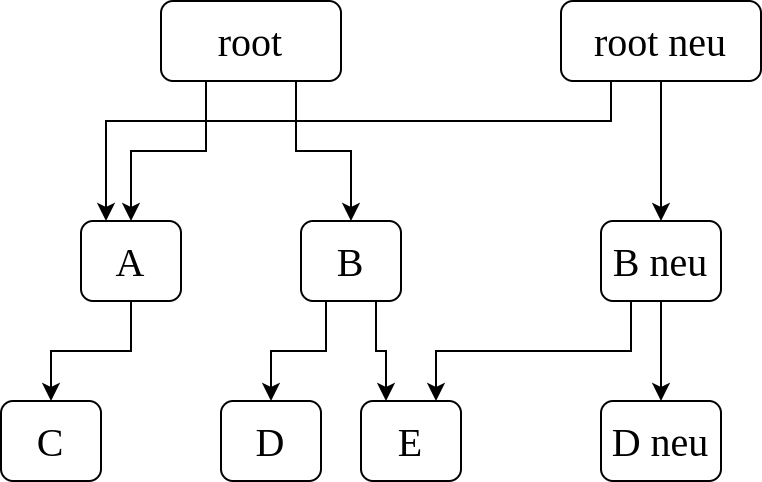
\includegraphics[height=5cm]{Bilder_Diagramme/COW.png}
    \caption{Funktionsprinzip COW nach der DESIGN.md}
    \label{fig:cowdesign}
\end{figure}
COW-Dateisysteme bieten eine langsamere, aber in der Praxis oft brauchbare Performance
im direkten Vergleich mit blockbasierten Dateisystemen, 
w"ahrend sie es gleichzeitig schaffen, Aktualisierungen durchzuführen,
ohne Datenänderungen direkt in einem Log oder Journal zu speichern. Gleichzeitig ist stets die
Dateisystemkonsistenz gew"ahrleistet. \\
\fig{fig:cowdesign} zeigt das Prinzip der Organisation anschaulich. Daten werden
bei COW-Dateisystemen oft in (balancierten) B"aumen gespeichert. Dies bezieht sich 
sowohl auf eine einzelne Datei, als auch auf z. B. Verzeichnisstrukturen.
Der gro"se Nachteil von COW-Dateisystemen ist, dass immer ein gesamter Zweig aktualisiert werden muss
bis zur Wurzel, egal wie klein die "Anderung ist.
Wenn man beispielsweise Daten in Block D ändert, passiert Folgendes:
Es wird eine komplett neue Kopie erstellt namens \enquote{D neu}.
Weil \enquote{D neu} jetzt an einer ganz anderen Stelle auf dem Speichermedium liegt als das alte \enquote{D},
stimmt der Verweis im übergeordneten Ordner (Block B) nicht mehr.
Also muss auch ein neuer Ordnerblock \enquote{B neu} geschrieben werden,
der auf \enquote{D neu} zeigt.
Weil jetzt aber \enquote{B neu} an einer neuen Stelle liegt,
stimmt der Verweis im Root-Block nicht mehr.
Das System muss also zwingend auch einen brandneuen \enquote{root neu}-Block schreiben.
Eine Aktualisierung kann also zu einer weitaus größeren Menge an Schreibvorgängen kaskadieren,
als f"ur die urspr"unglichen Daten eigentlich n"otig gewesen w"are. 
Dieses Hochwandern der Änderungen bis ganz nach oben zur Wurzel braucht O(log n) Schritte,
wenn die Datei oder das System aus n Elementen besteht und in einem balancierten Baum organisiert ist.

\subsection{FAT-Dateisysteme}
Das FAT-Dateisystem wurde 1980 von Microsoft entwickelt und erstmals von MS-DOS unterstützt.
Es wurde ursprünglich als einfaches Dateisystem entwickelt, 
das für Disketten mit einer Größe von weniger als 500 KB geeignet war. 
FAT ist die Abkürzung für File Allocation Table (Dateizuordnungstabelle). 
Derzeit gibt es vier FAT-Untertypen: FAT12, FAT16, FAT32 und seit 2006 exFAT als Nachfolger \cite{FAT32}.
Im Laufe der Zeit wurden die Spezifikationen erweitert, 
um mit zunehmender Kapazität auch größere Speichermedien zu unterstützen.

\begin{table}[H]
    \centering
    \caption{Technische Adressierungsgrenzen der FAT-Dateisysteme\cite{MSLearnFS}}
    \label{tab:fat_limits}
    \smallskip
    \begin{tabular}{l l l p{5cm}}
    \toprule
    \textbf{Dateisystem} & \textbf{Max. Dateigröße} & \textbf{Max. Mediengröße} & \textbf{Hauptsächlicher Einsatzzweck} \\
    \midrule
    \textbf{FAT12} & 16 MB & 16 MB   & Klassische 3,5-Zoll-Disketten (1,44 MB) \\
    \addlinespace
    \textbf{FAT16} & 2 GB & 2 GB  & MS-DOS-Systeme, frühe MP3-Player, alte CNC-Maschinen \\
    \addlinespace
    \textbf{FAT32} & 4 GB  & 2 TB  & USB-Sticks, ältere Kameras oder Konsolen \\
    \addlinespace
    \textbf{exFAT} & 512 TB oder mehr & 512 TB oder mehr & Moderne SDHC/SDXC-Speicherkarten, externe SSDs \\
    \bottomrule
    \end{tabular}
    \end{table}

\tab{tab:fat_limits} zeigt die maximal m"oglichen, \textit{"ublichen} Datei- und Mediengr"o"sen f"ur die FAT-Dateisysteme
und soll in erster Linie die Entwicklung der Spezifikation und die Probleme der "alteren Dateisysteme darstellen.
So ist es einem FAT32-Dateisystem beispielsweise nicht m"oglich eine 12 GB gro"se .iso-Datei aufzunehmen.\\
Wie ergeben sich die maximalen Datei- und Mediengr"o"sen?\\
Der Unterschied zwischen einem Sektor und einem Block wurde bereits erl"autert: 
Der Sektor ist die physisch kleinste adressierbare Einheit, 
w"ahrend der Block die logisch kleinste adressierbare Einheit ist. Im Kontext der FAT-Dateisysteme wird
der Block allerdings Cluster genannt, w"ahrend der Begriff des Blocks meist im Unix-Kontext "ublich ist. 
FAT12 stehen 12 Bits, FAT16 16 Bits und FAT32 28 Bits f"ur die Adressierung der Cluster zur Verf"ugung.
Mit gr"o"seren Clustergr"o"sen ergibt sich also eine gr"o"sere Mediengr"o"se. 
Gro"se Cluster haben allerdings den Nachteil, dass sehr kleine Dateien mindestens so gro"s werden wie die Clustergr"o"se.
Weiterhin wurden Clustergr"o"sen immer gedeckelt, "ublicherweise mit 32 KB Maximalgr"o"se f"ur FAT16 und FAT32.
Dies f"uhrt bei FAT16 zu den genannten 2 GB und bei FAT32 zu 8 TB maximaler Mediengr"o"se.
Hinzu kommt allerdings eine weitere Limitierung: Der MBR enth"alt die Partitionstabelle. Dieser z"ahlt allerdings
in 512 Byte gro"sen Sektoren und ihm steht lediglich ein Feld von 32 Bit f"ur die Adressierung zur Verf"ugung.
Folglich kann das FAT32-Dateisystem zwar ein gr"o"seres Medium unterst"utzen, wird dann aber von der MBR-Partitionstabelle
gebremst \cite{MSLearnFS}\cite{FAT32}. 

Die moderne L"osung dieser Limitierung liegt in der Verwendung des GUID Partition Table (GPT),
die ebenfalls viele weitere Vorteile zum MBR bringt wie beispielsweise eine erh"ohte Anzahl von Prim"arpartitionen und ein Backup
der Partitionstabelle am Ende des Speichermediums \cite{gpt}.

Die Dateigr"o"se bei FAT32-Systemen ist durch ein 32-Bit-Adressierungsfeld limitiert. Dieses z"ahlt in Bytes, wodurch sich
die charakteristischen 4 GB Dateigr"o"se ergeben, die f"ur heutige Zwecke manchmal nicht ausreichend sind\cite{MSLearnFS}\cite{FAT32}.
Zu diesem Zweck wurde mit exFAT als moderne FAT-Variante 2006 eingef"uhrt.

\subsubsection{Funktionsweise}
Die Funktionsweise soll im Rahmen dieser Arbeit nur schemenhaft aufgegriffen werden.

\begin{figure}[H]
    \centering
    \fbox{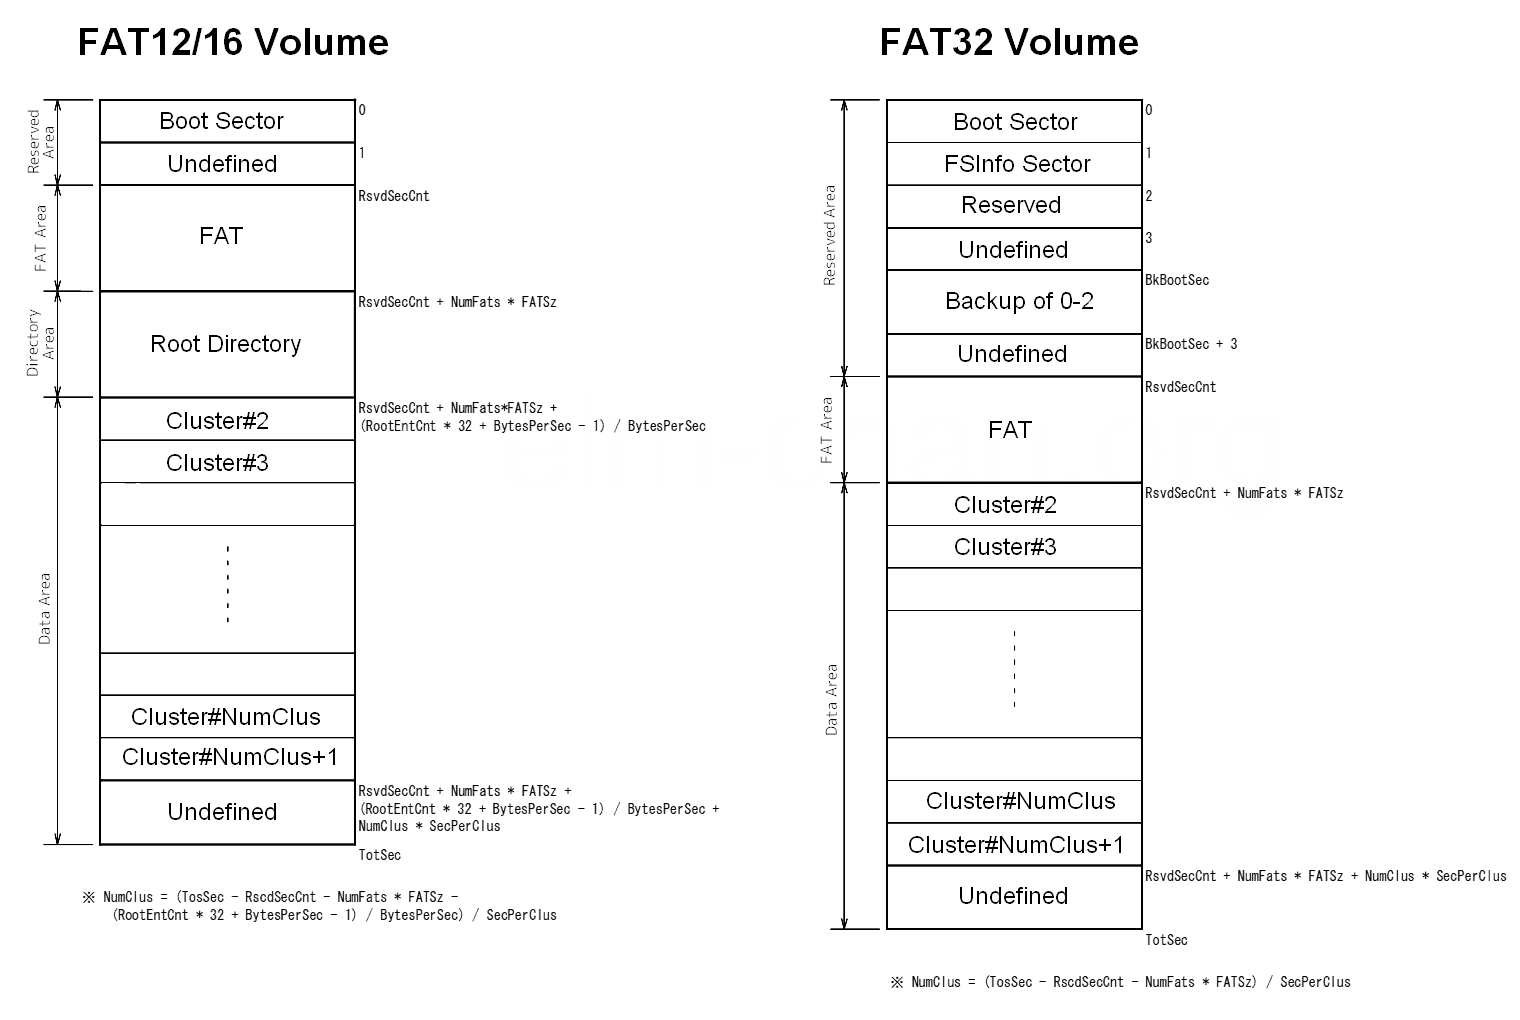
\includegraphics[width=\textwidth]{BilderExt/fat_map.png}}
    \caption{Struktur der FAT-Dateisysteme \cite{fatmap}}
    \label{fig:fatmap}
\end{figure}

\fig{fig:fatmap} zeigt die Struktur der FAT-Dateisysteme.
\hyperref[sec:fatfs]{ChaN} unterteilt das Dateisystem dabei in folgende Bereiche \cite{FAT32}:

\begin{itemize}
    \item \textbf{Reservierter Bereich:} Enth"alt im BPB (BIOS Parameter Block) Konfigurationsparameter zur Partition wie z. B. Sektorgr"o"se, Sektoranzahl pro Cluster, oder die Anzahl der FAT-Kopien.
    \item \textbf{FAT (File Allocation Table):} Tabelle mit einem Eintrag pro Cluster; verkettet Cluster zu Dateien und markiert freie Cluster.
    \item \textbf{Root-Verzeichnis:} Bei FAT12/16 fest, bei FAT32 ein normales Verzeichnis, also nicht als fester Bereich vorhanden. Enthält Dateieinträge (Name, Größe, Startcluster, Attribute).
    \item \textbf{Datenbereich:} Die eigentlichen Cluster, in denen Dateiinhalte liegen.
\end{itemize}

Der namensgebende Bereich, die File Allocation Table (FAT), ist oft in zweifacher Ausf"uhrung vorhanden, wobei das Feld 
\cpp{BPB_NumFATs} im BPB letztlich entscheidet, wie viele Kopien vorhanden sind. 
Dateien sind als verkettete Liste von Clustern gespeichert; die FAT gibt jeweils an, welcher Cluster auf welchen folgt.
Wenn z. B. eine Datei mit dem Cluster 7 anf"angt, dann steht in der FAT, dass auf Cluster 7 bspw. Cluster 12 folgt, dann Cluster 47 und 
zuletzt ein EOF (End Of File). Ein Defekt der FAT geht daher mit erheblichen Datenverlusten einher.
Die FAT \enquote{kennt} allerdings weder Dateinamen noch Dateiinhalt.
Die eigentlichen Daten befinden sich im Datenbereich. Dateinamen und Metadaten wie Attribute und Gr"o"se werden dort
in einem FAT-Verzeichniseintrag gespeichert (FAT Directory), wobei damit sowohl gew"ohnliche Dateien
gemeint sind als auch das, was gemeinhin unter einem \enquote{Verzeichnis} bekannt ist. In diesem FAT-Verzeichniseintrag
steht auch das Startcluster, sodass mit diesem und der File Allocation Table in Kombination eine Datei zusammengesetzt
werden kann. \\
Das Funktionsprinzip des FAT-Dateisystems ist verh"altnism"a"sig simpel, bringt aber mindestens zwei Schwachstellen
mit sich. Das erste Problem betrifft die sogenannte Fragmentierung: Wenn Dateien gel"oscht und neue Dateien erstellt werden, 
dann f"ullt FAT die L"ucken im Datenbereich jeweils mit dem nächsten freien Cluster auf,
den es findet. Eine Datei kann dadurch stark über den Datenträger verstreut werden. Zusammenh"angende Daten 
haben allerdings bei den allermeisten Datentr"agern schnellere Abruf- und Schreibzeiten. \\
Weiterhin ist auch klar geworden, dass die FAT ein fester Bereich am Anfang des Datentr"agers ist.
Da diese bei jeder Dateioperation aktualisiert wird, f"uhrt dies unweigerlich zum bereits vielfach erw"ahnten 
Wear Leveling Problem auf flashspeicherbasierten Medien.


\subsection{FatFs}\label{sec:fatfs}
\subsubsection{Einleitung}
FatFs ist ein plattformunabhängiges, quelloffenes Software-Modul zur Implementierung von FAT/exFAT-Dateisystemen in ressourcenbeschränkten, eingebetteten Systemen. 
Es wurde von dem Entwickler ChaN \cite{fatfs} entworfen und zeichnet sich durch einen extrem geringen Speicherbedarf sowohl im Programm- als auch im Arbeitsspeicher aus.
Das Modul ist vollständig in ANSI C (C89) geschrieben. 
Dadurch ist es hardwareunabhängig auf praktisch jedem gängigen Mikrocontroller 
(z. B. AVR, PIC oder STM32) ohne "Anderungen des Codes direkt lauffähig.\\ 
Die Architektur trennt das Dateisystem strikt in zwei logische Schichten: 
Das Application Interface stellt der Anwendung abstrakte, bekannte Funktionen zur Datei- und Verzeichnisverwaltung 
wie \cpp{f_open}, \cpp{f_read}, \cpp{f_write} und \cpp{f_close} zur Verfügung, 
während das Media Access Interface (Disk I/O) die Hardware vollkommen vom Dateisystem entkoppelt. 

\subsubsection{Implementierung}
\begin{figure}[H]
    \centering
    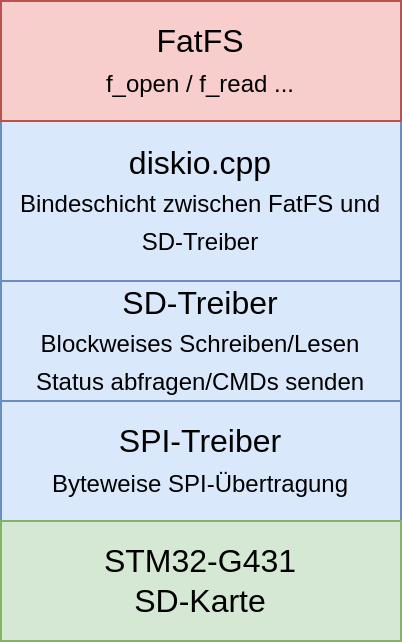
\includegraphics[height=8cm]{Bilder_Diagramme/FatFSstack.png}
    \caption{Implementierungsstack f"ur das FatFS-Dateisystem}
    \label{fig:fatfsimplement}
\end{figure}
%  zeigt den gesamten Implementierungsstack f"ur FatFS und somit FAT-Dateisysteme
% auf einem STM32G431. Alles, was sich in der Abbildung unter FatFS befindet muss auf die ein oder andere
% weise bereitgestellt und/oder implementiert werden. Dabei implementiert die Datei diskio.cpp (in den allermeisten
% F"allen ist es diskio.c) die n"otigen Funktionen, damit FatFS den Blockspeicher bedienen kann.
\fig{fig:fatfsimplement} zeigt den vollständigen Implementierungsstack für die Verwendung 
von FatFs und damit für den Zugriff auf ein FAT-Dateisystem auf dem STM32G431. 
Alle in der Abbildung unterhalb von FatFs dargestellten Schichten m"ussen implementiert bzw. bereitgestellt werden. 
Die Datei \\
\texttt{src/diskio.cpp} (in den meisten Implementierungen \texttt{diskio.c})
stellt dabei die von FatFs ben"otigte Schnittstelle zum darunterliegenden Blockgerät, hier SD-Karte, bereit.
Sie übersetzt die von FatFs angeforderten Lese-, Schreib- und Statusoperationen in die entsprechenden Funktionen
des verwendeten Treibers.

\begin{listing}[H]
        \begin{minted}[
            frame=lines,      % Rahmenlinien oben und unten
            framesep=2mm,     % Abstand zum Rahmen
            baselinestretch=1.2,
            bgcolor=lightgray!20, % Hintergrundfarbe
            fontsize=\footnotesize,
            linenos           % Zeilennummern aktivieren
        ]{cpp}
    DSTATUS disk_initialize(BYTE pdrv);
    DSTATUS disk_status(BYTE pdrv);
    DRESULT disk_read(BYTE pdrv, BYTE* buff, LBA_t sector, UINT count);
    DRESULT disk_write(BYTE pdrv, const BYTE* buff, LBA_t sector, UINT count);
    DRESULT disk_ioctl(BYTE pdrv, BYTE cmd, void* buff);
    
        \end{minted}
\caption{Funktionen, die in der \texttt{src/diskio.cpp} implementiert werden mussten}
\label{listing:diskioimplement}
\end{listing}

\coderef{listing:diskioimplement} zeigt die Funktionen, die f"ur FatFs implementiert werden m"ussen.
Zus"atzlich musste auch noch \cpp{DWORD get_fattime} implementiert werden, da jede FAT-Datei einen 
Zeitstempel braucht. Da die vorhandene Platine keine Echtzeituhr mitbringt, besitzt jede geschriebene
Datei einen fixen Zeitstempel, der auf den 1. Januar 2026 datiert wurde. 
Die Funktion findet sich in der Datei \texttt{src/fatfs\_time.cpp},
da sie thematisch nicht zu den anderen Funktionen in der \texttt{src/diskio.cpp} passt. \\
Bei den restlichen Funktionen ist die Hauptaufgabe, die Funktionen aus der \texttt{src/sdcarddriver.hpp} korrekt
aufzurufen.



\begin{listing}[H]
    \begin{minted}[
        frame=lines,      % Rahmenlinien oben und unten
        framesep=2mm,     % Abstand zum Rahmen
        baselinestretch=1.2,
        bgcolor=lightgray!20, % Hintergrundfarbe
        fontsize=\footnotesize,
        linenos           % Zeilennummern aktivieren
    ]{cpp}

template<typename Config>
DRESULT SD_disk_read(BYTE* buff, LBA_t sector, UINT count)
{

    uint8_t result;

    if (count == 1)
    {
        result = SD_ReadBlock<Config>(sector, buff);
    }
    else
    {
        result = SD_ReadBlocks<Config>(sector, count, buff);
    }

    //The SD_INIT_OK is my enum... the other RES stuff is FatFS, just to be clear
    if (result != SD_READ_OK) return RES_ERROR;


    return RES_OK;
}
    \end{minted}
\caption{Implementierung SD\_disk\_read}
\label{listing:cpp-diskread}
\end{listing}

\coderef{listing:cpp-diskread} zeigt beispielhaft die Implementation von \cpp{SD_disk_read},
welches wiederum in der urspr"unglichen Funktion \cpp{disk_read} aufgerufen wird. Da im
Treiber Template-Funktionen verwendet werden, die urspr"unglich von FatFs zur Verf"ugung gestellten
Funktionen sich aber in einer \cpp{extern "C"} Umgebung befinden, ist ein zweistufiger Prozess
mit einer Helferfunktion notwendig. In der eigentlichen \cpp{disk_read} wird noch das Argument
\cpp{BYTE pdrv} "ubergeben, was entscheidet, welches physische Laufwerk benutzt werden soll.
In unserem Fall bleibt die Wahl zwischen den beiden SD-Kartenslots: der SPI1-Peripherie mit \cpp{pdrv=0}
und der SPI3-Peripherie mit \cpp{pdrv=1}.\\
Der \coderef{listing:cpp-diskread} hingegen zeigt, dass sich die ben"otigten Aufrufe f"ur FatFs fast
direkt in Funktionsaufrufe aus der \texttt{src/sdcarddriver.hpp} "ubersetzen lassen. \\
An dieser Stelle kommt es auch zu dem bereits erw"ahnten Namenskonflikt bei den Argumenten:
So wird bei der Funktion \cpp{SD_ReadBlock} das Argument \texttt{sector} eingef"ugt, 
obwohl die Funktion das Argument \texttt{block} verlangt. In diesem Zusammenhang sind beide gleichbedeutend.


\subsubsection*{ffconf.h}

Die Datei \texttt{FatFs/ffconf.h} ist die zentrale Konfigurationsdatei des FatFs-Moduls. 
Über den C-Präprozessor lässt sich der Funktionsumfang auf die Hardware-Ressourcen des Mikrocontrollers zuschneiden.
Im Folgenden sollen die Konfigurationsm"oglichkeiten durch eine kleine Auswahl an Optionen verdeutlicht werden: 

\begin{itemize}
    \item \textbf{Anpassbarer Funktionsumfang:}
    \begin{itemize}
        \item \texttt{FF\_FS\_READONLY}: Schaltet das Schreiben komplett ab.
        \item \texttt{FF\_FS\_MINIMIZE}: Entfernt gezielt ungenutzte APIs wie z. B. die Verzeichnisoperationen (\texttt{f\_mkdir}, \texttt{f\_opendir}) oder Suchfunktionen.
        \item \texttt{FF\_USE\_MKFS}: Aktiviert oder deaktiviert die Formatierungsfunktion \texttt{f\_mkfs}.
        \item \texttt{FF\_USE\_FIND}: Aktiviert Suchfunktionen wie \texttt{f\_findfirst()} und \texttt{f\_findnext()}.
    \end{itemize}
    
    \item \textbf{Dateinamen und Zeichenkodierung:}
    \begin{itemize}
        \item \texttt{FF\_USE\_LFN}: Schaltet die Unterstützung für lange Dateinamen frei.
        \item \texttt{FF\_CODE\_PAGE}: Legt die Codepage fest, um Sonderzeichen korrekt darzustellen.
        \item \texttt{FF\_LFN\_UNICODE}: Aktiviert Unicode-Unterstützung für Dateinamen.
    \end{itemize}
    
    \item \textbf{Systemeinstellungen:}
    \begin{itemize}
        \item \texttt{FF\_FS\_TINY}: Reduziert den RAM-Bedarf pro Datei, indem interne Buffer gemeinsam genutzt werden.
        \item \texttt{FF\_FS\_EXFAT}: Aktiviert die Unterstützung des exFAT-Dateisystems.
    \end{itemize}
\end{itemize}

Darüber hinaus stellt FatFs zahlreiche weitere Konfigurationsoptionen bereit, wie z. B. die Unterst"utzung 
f"ur mehrere Partitionen oder die Unterst"utzung f"ur GPT-Partitionstabellen.
Dadurch lässt sich das Dateisystem flexibel an die Anforderungen der jeweiligen
Embedded-Anwendung anpassen.
Eine vollst"andige Auflistung findet sich einerseits direkt in der \texttt{FatFs/ffconf.h} mit hilfreichen Kommentaren,
andererseits auf der \href{https://elm-chan.org/fsw/ff/doc/config.html}{offiziellen Webseite des Entwicklers}.

FatFs wurde in dieser Arbeit "uberwiegend im vorkonfigurierten Umfang eingesetzt: 
Alle Standardfunktionen waren voll verf"ugbar (\texttt{FF\_FS\_MINIMIZE}=0), 
mkfs zur Formatierung wurde benutzt, exFAT wurde nicht
getestet. Au"serdem wurden Versuche sowohl mit langen
als auch mit kurzen Dateinamen durchgef"uhrt.


\subsection{LittleFS}


\subsubsection{Ziele von littlefs}

Die Entwickler des littlefs-Dateisystems nennen auf ihrer GitHub-Seite drei gro"se Vorteile ihres Dateisystems:
\begin{itemize}
    \item \textbf{Ausfallsicherheit bei Stromausfall} 
    \item \textbf{Verschleißregulierung des Flashspeichers (Wear Leveling)} 
    \item \textbf{Begrenzter RAM/ROM-Bedarf}
\end{itemize}

Das Design von littlefs wurde in Hinblick auf die Gew"ahrleistung dieser drei Hauptpunkte optimiert
und soll im Folgenden n"aher beleuchtet werden.


\subsubsection{Funktionsweise} \label{sec:funclittle}
Die Funktionsweise von littlefs wird in der bereits zitierten \href{https://github.com/littlefs-project/littlefs/blob/master/DESIGN.md}{DESIGN.md}
erl"autert. Diese ist "au"serst komplex und kann in diesem Rahmen nur schemenhaft erl"autert werden:
Die \enquote{Superblock-Ebene}, also die oberste Strukturebene des Dateisystems, nutzt eine modifizierte Form
des bereits erl"auterten COW (Copy-on-Write) f"ur die grunds"atzliche Neubeschaffung und Strukturierung von Bl"ocken. 
Das sogenannte CObW (Copy-On-bounded-Write) f"uhrt einen Z"ahler ein, sodass nicht bei jeder Modifikation
der gesamte Baum neu geschrieben werden muss wie bei COW, sondern nur alle N male. Bis zur N-ten Modifikation
bleibt der alte Baum g"ultig. Dies reduziert den Aufw"artskaskadierungsaufwand, den COW-Dateisysteme mit sich bringen,
um den Faktor N. CObW wird bei littlefs also f"ur die gro"sen Datenstrukturen verwendet und bringt 
den Vorteil des Wear-Levelings mit sich sowie eine Dateikonsistenzgarantie bei unerwartetem Stromausfall. \\
Auf Dateiebene nutzt littlefs unterschiedliche Mechanismen
f"ur die tats"achlichen Dateiinhalte und die Metadaten (Dateiname, Gr"o"se, etc.).
F"ur den Dateiinhalt wird eine sogenannte \enquote{CTZ skip list} verwendet, 
die man sich als eine Erweiterung der Datenstruktur der verketteten Liste vorstellen kann.

\begin{table}[h]
    \centering
    \caption{Zahl von Zeigern in der \enquote{CTZ skip list} in Abhängigkeit des Blockindexes.}
    \begin{tabular}{c c c c}
        \hline
        Blockzahl & Blockzahl(bin) & CTZ & Zeiger \\
        \hline
        1 & 0001 & 0 & 1 \\
        2 & 0010 & 1 & 2 \\
        3 & 0011 & 0 & 1 \\
        4 & 0100 & 2 & 3 \\
        5 & 0101 & 0 & 1 \\
        6 & 0110 & 1 & 2 \\
        7 & 0111 & 0 & 1 \\
        8 & 1000 & 3 & 4 \\
        \hline
    \end{tabular}
    \label{tab:ctz-pointers}
\end{table}

Der gro"se Unterschied ist, dass die \enquote{skip list} zus"atzliche Zeiger einf"uhrt, die Elemente
"uberspringen k"onnen. In einer gew"ohnlichen \enquote{skip list} ist es zufallsbasiert, wie viele Zeiger
ein bestimmter Eintrag hat. Die CTZ skip list (Count Trailing Zeros) nutzt als Zeigerverteilung einfach
die Anzahl der abschlie"senden Nullen einer Zahl in Bin"ardarstellung.
\tab{tab:ctz-pointers} zeigt die Verteilung beispielhaft f"ur die Bl"ocke 1 bis 8.
Der Vorteil dieser Datenstruktur ist die Suchlaufzeit
von O($log(n)$) f"ur einen speziellen Block, w"ahrend die Traversion durch alle Bl"ocke einer Datei in einer Laufzeit von O($n \cdot log(n)$)
m"oglich ist und ein Anh"angen eines Blocks an eine Datei nur einen Schritt (O(1)) ben"otigt. 
Eine r"uckw"arts verkettete Liste h"atte beispielsweise den Nachteil, dass die Traversion durch
alle Bl"ocke O($n^2$) Schritte ben"otigt, w"ahrend eine vorw"arts verkettete Liste nicht an eine Datei Bl"ocke anf"ugen kann,
ohne mindestens einen vorherigen Block zu modifizieren. Andere beliebte Datenstrukturen wie balancierte B"aume haben Nachteile
bez"uglich einer beschr"ankten RAM-Nutzung, wie sie bei eingebetteten Systemen gefordert ist. \\ 
F"ur Metadaten wird ein \enquote{two-block log} verwendet.

\begin{figure}[H]
    \centering
    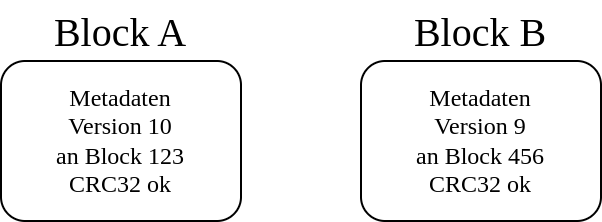
\includegraphics[height=6cm]{Bilder_Diagramme/littlefsmetadata.png}
    \caption{Prinzip \enquote{two-block log}}
    \label{fig:littlefsmetaidea}
\end{figure}

\fig{fig:littlefsmetaidea} zeigt die Idee hinter dem \enquote{two-block log} f"ur Metadaten auf.
Die Metadaten stehen zu jedem Zeitpunkt in zwei Bl"ocken, die in sich eine begrenzte
Anzahl an Commits zulassen. Ein Commit kann beispielsweise eine "Anderung der Metadaten beinhalten oder 
ein Hinzuf"ugen von Metadaten. Jeder Commit wird mit einer CRC32 abgeschlossen; ist diese nicht g"ultig,
so wird der Commit verworfen. Das Prinzip ist also das eines Logging-Dateisystems, allerdings beschr"ankt
in der Gr"o"se. Sobald einer der Bl"ocke voll ist, wird er auf den anderen Block komprimiert. Diesem wird
dann eine neue Revisionsnummer gegeben und fortan ist dies der neue aktive Logblock.
Der Vorteil, den das System mit sich bringt, ist die dauerhafte Konsistenz der Metadaten, da nichts
"uberschrieben wird, sondern zu jedem Zeitpunkt eine korrekte Version der Daten existiert. Weiterhin
bringt das Logging durch die Begrenzung der Gr"o"se des Logs eine nahezu konstante Laufzeit mit sich.
Dadurch, dass aber "uberwiegend mit Logs gearbeitet wird, ist fundamental der Anspruch an Wear-Leveling erf"ullt.  
Zum Vergleich: FatFs "uberschreibt seine Metadaten an Ort und Stelle und gef"ahrdet damit die
gesamte Dateiintegrit"at, falls die Schreiboperation scheitert. Ebenfalls ist das nicht
optimal f"ur das Wear-Leveling.\\
Grunds"atzlich gilt f"ur Metadaten bei littlefs der Begriff der Atomarität:
Entweder die Operation wird vollst"andig ausgef"uhrt oder gar nicht. 
Die CRC32-Pr"ufsumme gew"ahrleistet die Vollst"andigkeit eines Commits.


\begin{figure}[H]
    \centering
    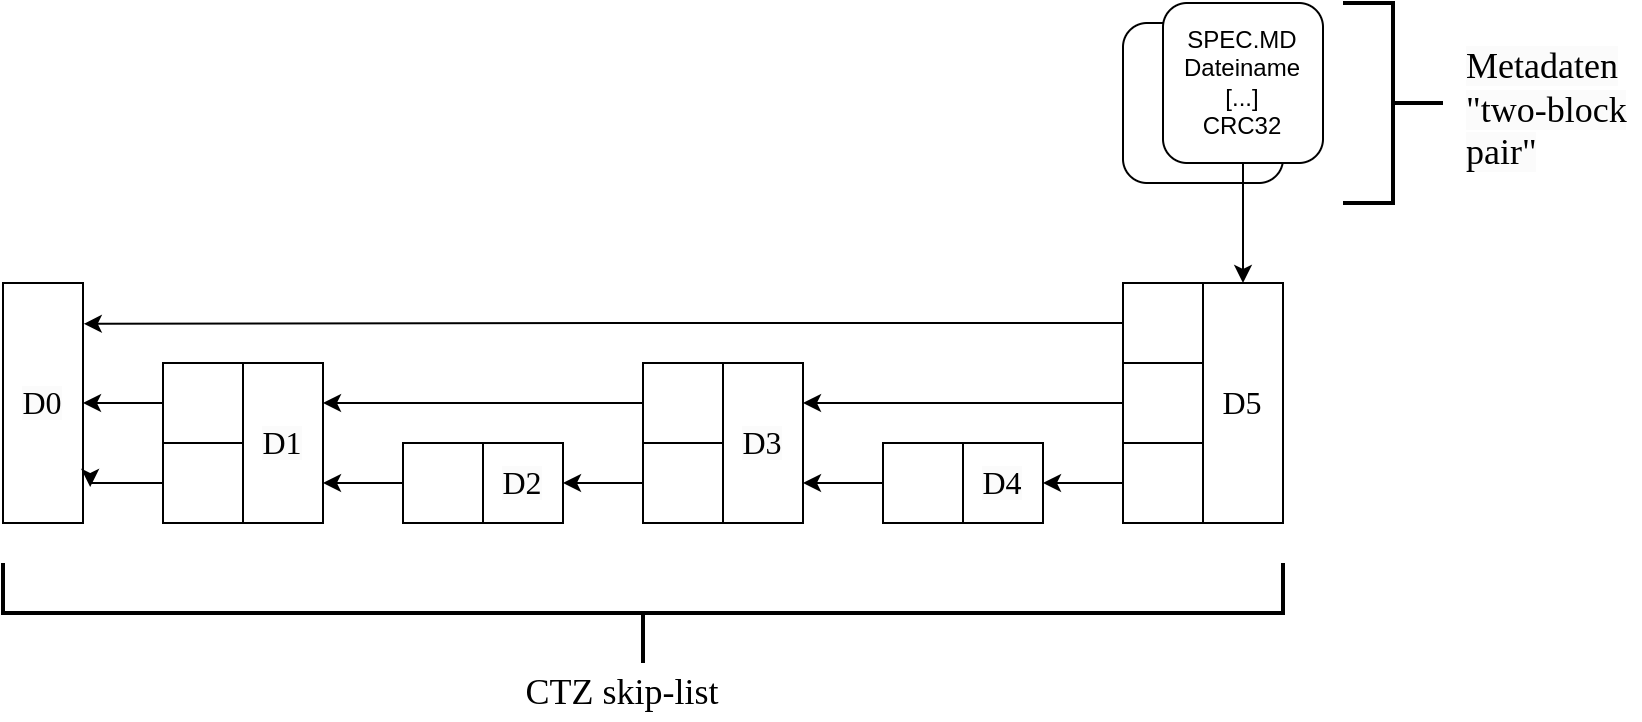
\includegraphics[height=7cm]{Bilder_Diagramme/littlefsgesamt.png}
    \caption{Prinzip des Dateiaufbaus bei littlefs}
    \label{fig:littlefsall}
\end{figure}

\fig{fig:littlefsall} zeigt anschaulich den prinzipiellen Aufbau einer Datei in littlefs nach dem
erl"auterten Prinzip. \\

Eine wichtige, in der DESIGN.md erw"ahnte Funktionalit"at ist das Zur"ucklesen des
geschriebenen Buffers und ein Vergleichen der Nachricht. Damit kann littlefs feststellen, ob das 
Schreiben tats"achlich geklappt hat oder m"oglicherweise ein Schreibfehler vorliegt. Im Falle von 
Flashspeicher k"onnte in diesem Falle ein Badblock vorliegen, also ein defekter Speicherblock.
Das Dateisystem probiert daher das Schreiben auf einem anderen Block und zwar so lange, bis
es die Nachricht korrekt zur"ucklesen kann.   



\subsubsection{Implementierung}

\begin{figure}[H]
    \centering
    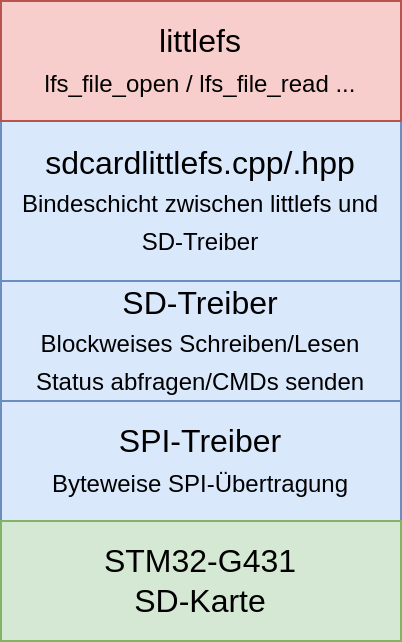
\includegraphics[height=8cm]{Bilder_Diagramme/littlefsstack.png}
    \caption{Implementierungsstack f"ur das littlefs-Dateisystem}
    \label{fig:littlefsimplements}
\end{figure}

\fig{fig:littlefsimplements} zeigt den Implementierungsstack f"ur das littlefs-Dateisystem.
Im Grunde genommen nutzt littlefs genauso wie FatFs die Blockschreib- und Lesefunktionen des
SD-Kartentreibers. Die Datei, die littlefs und SD-Kartentreiber verbindet, 
findet sich unter \texttt{src/sdcardlittlefs.cpp}.
Leider besteht die haupts"achliche Dokumentation f"ur littlefs aus
Kommentaren in der Quelldatei \texttt{littlefs/lfs.h}. 
Zus"atzlich gibt es auf der GitHub-Seite ein unvollst"andiges Beispiel und
die bereits erw"ahnte ausf"uhrliche Erkl"arung des Prinzips in der
\href{https://github.com/littlefs-project/littlefs/blob/master/DESIGN.md}{DESIGN.md}.
Kurzum sind die vorhandenen Informationen im Gegensatz zu FatFs sehr beschr"ankt,
sodass zwar eine funktionierende, aber m"oglicherweise keine optimale Implementierung 
der Bindeschicht in der \texttt{src/sdcardlittlefs.cpp} gew"ahrleistet werden konnte.

\subsubsection{littlefs FUSE Wrapper}
W"ahrend sich mit FAT formatierte SD-Karten problemlos an jedem Desktop-PC mit jedem 
erdenklichen Betriebssystem auslesen lassen, existiert f"ur littlefs das 
\href{https://github.com/littlefs-project/littlefs-fuse}{littlefs FUSE Wrapper} Projekt.
Nach erfolgreichem Kompilieren des Projektes l"asst sich unter Linux beispielsweise mit 
\texttt{sudo ./lfs /dev/mmcblk0 mount/ -o allow\_other} das Dateisystem einh"angen und
mit kleinen Einschr"ankungen nutzen. Zu den Einschr"ankungen geh"ort,
dass littlefs keine Zeitstempel f"ur Dateien anlegt und auch kein System f"ur spezielle
Berechtigungen existiert. \\
An dieser Stelle stellt sich f"ur die Praxis ebenfalls die Frage, ob der Endnutzer mit dem Dateisystem
in Ber"uhrung kommen wird. W"ahrend die Einrichtung des littlefs FUSE Wrapper Projektes  
f"ur technisch versierte und mit GitHub vertraute Personen problemlos in weniger als einer Stunde 
m"oglich ist, ist es f"ur normale Endnutzer ungeeignet und "uberfordernd. Littlefs ist
also kein Dateisystem, das f"ur Ger"ate wie beispielsweise Digitalkameras oder Oszilloskope
zu empfehlen w"are, wo dem Endnutzer eine Kompatibilit"at mit dem Dateisystem 
garantiert werden sollte.

\section{Vergleich littlefs, FatFs und direkter Blockadressierung}
Im Folgenden wird die direkte Blockadressierung als \enquote{NoFs} bezeichnet.

\subsection{RAM- und Flashverbrauch}\label{sec:ramflash}
\tab{tab:flash-ram} ist die Auswertung der Ausgabe des Compilers \enquote{arm-none-eabi-gcc} bei
unterschiedlichen Optimierungsstufen. \\
F"ur FatFs wurde eine kleine Standardkonfiguration verwendet.
Das bedeutet konkret, dass alle Standardfunktionen vorhanden sind (FF\_FS\_MINIMIZE=0),
aber der Support f"ur lange Dateinamen \\ (FF\_USE\_LFN=0) abgeschaltet ist. \\
Der statische RAM-Verbrauch h"alt sich "uber alle Dateisysteme
recht stabil im Bereich von 2 KB und schwankt auch nach der Compileroptimierung nicht sonderlich.
Hiervon ausgenommen ist FatFs, dessen statischer RAM-Verbrauch in optimierten Builds um fast 500 Bytes sinkt
im Vergleich zum unoptimierten Build, sodass lediglich 1,5 KB an statischem RAM verbraucht werden.
Da auch FatFs intern dieselben Treiber verwendet wie NoFs und littlefs, ist dies ein Hinweis darauf,
dass die internen Buffer f"ur FatFs auf dem Stack allokiert werden, w"ahrend NoFs und littlefs statische
Buffer nutzt, die der Compiler beim Build im .data oder .bss Segment verordnen und somit anzeigen kann.\\
Weitere Untersuchungen des FatFs-Dateisystems haben gezeigt, dass sich der Hauptbuffer von FatFs in
der Struktur \texttt{FIL} befindet und diese eine Gr"o"se von 552 Bytes aufweist. Ob der Buffer also auf dem Stack liegt oder
im statischen/globalen Segment allokiert wird, liegt in diesem Fall also in der Hand des Programmierers,
was f"ur Systeme, die ihren RAM-Bereich fest aufteilen, sehr n"utzlich sein kann. Dies ist selbstverst"andlich
auch der Fall f"ur NoFs.
\\
Der Flashverbrauch entspricht den Erwartungen:
Er ist bei NoFs am kleinsten und bei littlefs am h"ochsten. Das h"angt mit der Komplexit"at
des Dateisystems zusammen. W"ahrend FatFs ein relativ simples, blockbasiertes Dateisystem ist,
fusioniert littlefs die Ideen der Journaling and Copy-on-Write Dateisysteme f"ur mehr Ausfallresilienz
und Wear-Leveling. Dies spiegelt sich im Speicherverbrauch f"ur den Programmspeicher wider.
NoFs verwendet in der kleinsten Variante etwa 2 KB, FatFs etwa 15 KB und littlefs etwa 35 KB Speicher auf dem Flash.
W"ahrend das f"ur den verwendeten STM32G431 mit 128 KB Flashspeicher kein Problem darstellt, so
gibt es zahlreiche kosteng"unstige STM-Modelle wie beispielsweise Modelle aus der STM32C0-Serie,
die nur "uber 32 KB Programmspeicher verf"ugen und somit kein littlefs in dieser Konfiguration nutzen k"onnen. \\
Ebenfalls interessant ist zu sehen, dass die Programmgr"o"se bei der Optimierung \enquote{-O3} gr"o"ser ist als 
bei \enquote{-O2}. Dies h"angt damit zusammen, dass auf Ausf"uhrungsgeschwindigkeit optimiert wird statt auf Gr"o"se.
So werden beispielsweise Funktionen aggressiver geinlined, um Funktionsaufrufe zu sparen, was sich aber wiederum 
in einer h"oheren Programmgr"o"se widerspiegelt.


            \begin{table}[H]
                \centering
                \caption{Flash und statischer RAM der verschiedenen Dateisysteme bei unterschiedlicher Compiler-Optimierungsstufe}
                \label{tab:flash-ram}
                \begin{tabular}{|l|c|c|c|}
                \hline
                \textbf{Optimierungsstufe} & \textbf{Dateisystem} & \textbf{Flash (Bytes)} & \textbf{Statischer RAM (Bytes)} \\
                \hline
                \multirow{3}{*}{-O0} & littlefs & 57504 & 2184 \\
                                      & NoFs     & 13424 & 2512 \\
                                      & FatFs    & 28304 & 2008 \\
                \hline
                \multirow{3}{*}{-O1} & littlefs & 39716 & 2168 \\
                                      & NoFs     &  3120 & 2080 \\
                                      & FatFs    & 19316 & 1576 \\
                \hline
                \multirow{3}{*}{-O2} & littlefs & 39308 & 2168 \\
                                      & NoFs     &  2404 & 2080 \\
                                      & FatFs    & 17536 & 1576 \\
                \hline
                \multirow{3}{*}{-O3} & littlefs & 47596 & 2168 \\
                                      & NoFs     &  2720 & 2080 \\
                                      & FatFs    & 18612 & 1576 \\
                \hline
                \multirow{3}{*}{-Os} & littlefs & 35148 & 2168 \\
                                      & NoFs     &  2124 & 2080 \\
                                      & FatFs    & 15044 & 1576 \\
                \hline
                \end{tabular}
                \end{table}



\subsection{Versuch 1: Analyse der Schreibfehlerraten mittels bekannter Zeichenfolge}\label{sec:v1}



\begin{listing}[H]
    \begin{minted}[
        frame=lines,      % Rahmenlinien oben und unten
        framesep=2mm,     % Abstand zum Rahmen
        baselinestretch=1.2,
        bgcolor=lightgray!20, % Hintergrundfarbe
        fontsize=\footnotesize,
        linenos           % Zeilennummern aktivieren
    ]{cpp}
    for(;;)
    {
        int tcnt_ms = TIM2->CNT/1000;
        std::snprintf(filename, sizeof(filename), "l_%06d_%06d_%08d.txt", 
        file_number, cnt_number, tcnt_ms);

        char msg[32];
        int msg_len = std::snprintf(msg, sizeof(msg), "Write %08d!\n", file_number);
        for (int j = 0; j < 64; j++)
        {
            std::memcpy(lfswritebuf + j * msg_len, msg, msg_len);
        }

        int res_open = lfs_file_open(&lfs_inst, &file, filename, LFS_O_RDWR | LFS_O_CREAT);
        if(res_open == LFS_ERR_OK)
        {
            lfs_file_write(&lfs_inst, &file, &lfswritebuf, sizeof(lfswritebuf));

            lfs_file_close(&lfs_inst, &file);
            file_number++;
        }
        cnt_number++;
    }
    \end{minted}
\caption{Hauptschleife aus \texttt{test/littlefs\_write\_test.cpp}}
\label{listing:littlefswritetest}
\end{listing}

\coderef{listing:littlefswritetest} zeigt die relevante Hauptschleife des Schreibtests f"ur das littlefs-Dateisystem.
Der Schreibtest f"ur das FatFs-Dateisystem ist analog dazu in \texttt{test/fatfs\_write\_test.cpp} vorhanden.
\fig{fig:versuch1loop} verdeutlicht den Ablauf anschaulich. 
Die aufgenommenen Testdaten finden sich im GitHub-Projektverzeichnis unter 
\href{https://github.com/miko8278/stm32-SPI-SD-card/tree/main/test\_data/Writetest1}{(root)/test\_data/Writetest1/}.
Die Auswertung erfolgte am station"aren Desktop-Computer. Dazu wurden kurze Pythonskripte erstellt, die
Dateigr"o"se und Integrit"at der Daten pr"ufen. Das relevanteste Skript ist hierbei 
\href{https://github.com/miko8278/stm32-SPI-SD-card/blob/main/test\_data/Writetest1/test\_readable.py}{(root)/test\_data/Writetest1/test\_readable.py}.
In der Auswertung zeigt sich, dass unter etwa 9000 littlefs-Dateien und rund 8000 FatFs-Dateien keine einzige Datei auch nur
einen einzigen messbaren Bitfehler aufweist, trotz fehlender CRC-Pr"ufsumme bei der SPI-Daten"ubertragung.
Somit kann anhand dieses Versuchs keine Aussage dar"uber getroffen werden,
ob ein Dateisystem zuverl"assiger mit Daten umgeht als das andere.
Gleichzeitig best"atigt der Versuch, dass die zugrunde liegenden Blockschreibfunktionen "uber eine Vielzahl von Aufrufen zuverl"assig arbeiten.

\begin{figure}[H]
    \centering
    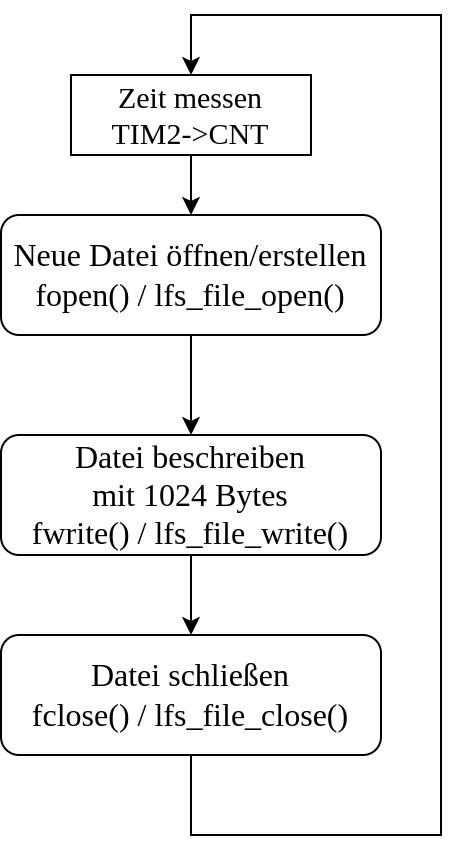
\includegraphics[height=8cm]{Bilder_Diagramme/Versuch1loop.png}
    \caption{Schreibzyklus f"ur eine 1024 Byte gro"se Versuchsdatei}
    \label{fig:versuch1loop}
\end{figure}

Tats"achlich war der Plan, etwa die zehnfache Menge an geschriebenen Daten f"ur diesen
Versuch zu erzeugen. Dies war durch kurze Messreihen von einer Minute abgesch"atzt worden.
W"ahrend des Schreibversuches ist klar geworden, dass deutlich weniger Dateien erstellt wurden
als zun"achst angenommen. 
Obwohl in dieser Arbeit vorrangig die Zuverl"assigkeit der Dateisysteme bez"uglich
der Datenintegrit"at untersucht werden sollte, ist es beispielsweise f"ur Logginganwendungen
unverzichtbar, ein konsistentes Verhalten beim Erstellen und Schreiben von Dateien zu erreichen.
Also wurde der Versuch um einen Zeitstempel im Dateinamen erweitert, sodass die Dauer des gesamten Zyklus
der Dateierstellung, wie in \fig{fig:versuch1loop} aufgezeigt, gemessen werden konnte.

\begin{figure}[H]
    \centering
    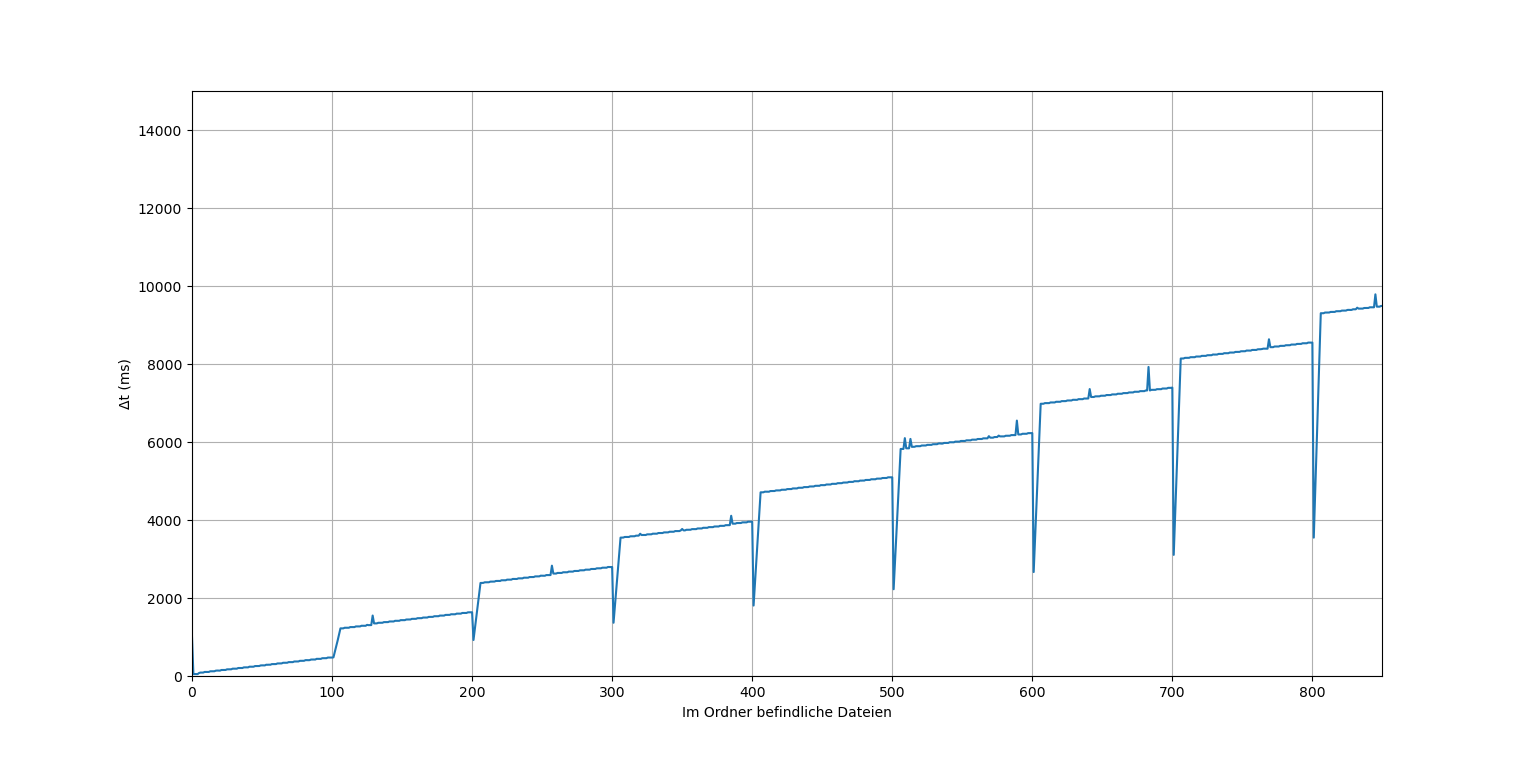
\includegraphics[width=\textwidth, trim=3cm 0cm 3cm 0cm, clip]{Bilder_Plot/1_fatfs_dateierstellzeit.png}
    \caption{Dauer der Neuerstellung von 1\,KB Dateien auf dem FatFs-Dateisystem}
    \label{fig:fatfstime}
\end{figure}

\fig{fig:fatfstime} zeigt die Dauer des Schreibvorgangs f"ur eine 1024 Byte Datei in Abh"angigkeit
davon, wie viele Dateien bereits erstellt wurden. Es zeigt sich eine klare lineare Abh"angigkeit mit einem 
auff"allig periodisch wiederkehrenden Muster.

\begin{figure}[H]
    \centering
    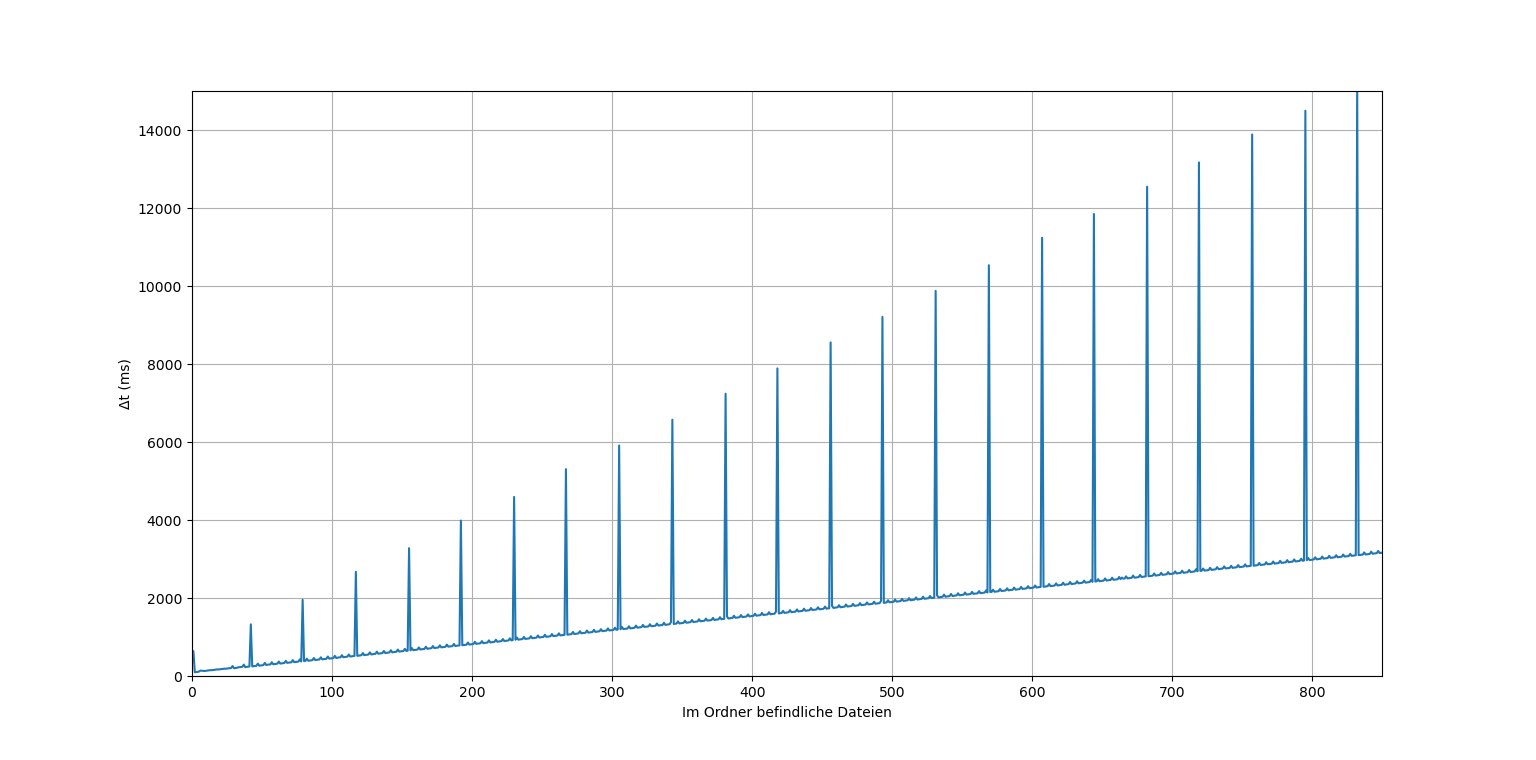
\includegraphics[width=\textwidth, trim=3cm 0cm 3cm 0cm, clip]{Bilder_Plot/2_littlefs_dateierstellzeit.png}
    \caption{Dauer der Neuerstellung von 1\,KB Dateien auf dem littlefs-Dateisystem}
    \label{fig:littlefstime}
\end{figure}

\fig{fig:littlefstime} zeigt dieselbe Messreihe f"ur das littlefs-Dateisystem.
Auch hier sehen wir einen konstanten, linearen Anstieg der Dateierstelldauer in Abh"angigkeit der bereits vorhandenen
Dateien. Zus"atzlich braucht das Dateisystem alle 38 Dateien einmalig deutlich l"anger f"ur die Erstellung einer Datei.
Eine m"ogliche Erkl"arung f"ur dieses Verhalten k"onnte der bereits erw"ahnte CObW-Mechanismus sein. Nach 38 Dateien w"are
der Zeitpunkt erreicht, an dem einmalig ein ganzer Zweig eines Baumes neu geschrieben werden muss.

W"ahrend hier der "Ubersichtlichkeit halber nur ein Auszug von rund 850 Dateien dargestellt ist, wurden alle vorhandenen
Messdaten untersucht. Sowohl f"ur littlefs als auch f"ur FatFs setzt sich das typische Muster mit linear steigender Dateierstelldauer fort.

Bei genauer Betrachtung der Werte f"allt auf, dass das FatFs-Dateisystem trotz geringerer Dateisystemkomplexit"at l"anger
f"ur die Erstellung von Dateien ben"otigt als littlefs. Die Vermutung lag nahe, dass das mit FatFs Option \enquote{LFN} (\enquote{Long File Names})
zusammenh"angt. Dies ist eine Erweiterung f"ur lange Dateinamen mit Unicode-Kodierung, die im klassischen FAT-Standard zun"achst
nicht vorgesehen war. Diese Form der Dateinamen belegt insgesamt mehr Speicher aufgrund komplexerer Kodierung. Es wurden daher noch einmal eine Messreihe mit FatFs im klassischen \enquote{SFN}, \enquote{Short File Name} oder auch 8.3 Format,
aufgenommen. Das Problem an diesem Format ist, dass nicht nur keine Umlaute f"ur Dateinamen funktionieren, sondern auch noch
alle Dateien in Gro"sbuchstaben aufgezeichnet werden und nur eine maximale L"ange von 8 Zeichen aufweisen d"urfen, sowie 3 weitere Zeichen
f"ur Dateiendungen wie \enquote{.txt}.
\fig{fig:dateierstellalle} best"atigt die Vermutung. Mit dem klassischen SFN-Format zeigt FatFs eine deutlich bessere Performance
beim Erstellen von Dateien als littlefs. 

\subsubsection*{Fazit Versuch 1}
Auch wenn in diesem Versuch keine Aussage "uber die Datenintegrit"at getroffen werden konnte, da die zugrunde liegende "Ubertragungsebene
fehlerfrei gearbeitet hat, so lassen sich dennoch wichtige Schl"usse f"ur den Umgang mit Dateien auf eingebetteten Systemen ziehen:
Bei der Speicherung von Daten ist es f"ur die Geschwindigkeit des Schreibzyklus vorteilhaft, diese in m"oglichst wenig Dateien zu b"undeln. 
Sollen dennoch separate Dateien erzeugt werden, so ist es vorteilhaft, diese ab einer gewissen Anzahl auf Unterordner aufzuteilen.
Eine m"ogliche Erkl"arung ist hierf"ur, dass die Dateisysteme vor dem Erstellen neuer Dateien den gesamten Inhalt des Ordners
zun"achst auslesen m"ussen. Wenn dieser eine komplexe Kodierung enth"alt wie im Falle von FAT32-LFN oder sehr viele Dateien, so schadet
das der Performance, insbesondere da auf eingebetteten Systemen die Speicherbuffer, mit denen gearbeitet wird, sehr klein sind. \\


\subsection{Versuch 2: Analyse der Schreibfehlerraten mittels bekannter Zeichenfolge und manipulierter Schreibfunktion}\label{sec:v2}
Versuch 2 folgt im Aufbau und in der Idee analog zu Versuch 1.
Aufgrund der hohen Zuverl"assigkeit der Schreibfunktionen wird nun allerdings eine gezielte Fehlerinjektion 
in den Schreibfunktionen des SD-Kartentreibers durchgef"uhrt,
bei der nach jeweils 5000 Bytes ein Byte modifiziert wird. Der Wert wurde so gew"ahlt, dass jeder 9. bis 10.
Block ein mit hoher Wahrscheinlichkeit falsches Byte enth"alt.
Da sowohl littlefs als auch FatFs diese Funktion als 
Basis nutzen, ist eine "Uberpr"ufung des Umgangs mit fehlerhaften Daten auf Dateisystemebene m"oglich. 


\begin{listing}[H]
    \begin{minted}[
        frame=lines,      % Rahmenlinien oben und unten
        framesep=2mm,     % Abstand zum Rahmen
        baselinestretch=1.2,
        bgcolor=lightgray!20, % Hintergrundfarbe
        fontsize=\footnotesize,
        linenos           % Zeilennummern aktivieren
    ]{cpp}
    // send 512 byte blockdata
    for (uint16_t i = 0; i < 512; i++) {
        //Injecting errors
        if(err_cnt == 5000) 
        { 
            //some random data
            //const_cast<uint8_t*>(buffer)[i] = 0xAA;
            SpiDriver<Config::SpiBase>::Transfer(0xAA);
            err_cnt = 0;
            continue;
        } 
        err_cnt++;
        SpiDriver<Config::SpiBase>::Transfer(buffer[i]);
    }
    \end{minted}
\caption{Modifizierter Teil der Funktion \texttt{SD\_WriteBlock} aus Datei \texttt{src/sdcarddriver.hpp}}
\label{listing:sdwriteblockmod}
\end{listing}

\coderef{listing:sdwriteblockmod} zeigt den modifizierten Teil der Schreibfunktion.
Die aufgenommenen Rohdaten finden sich in \href{https://github.com/miko8278/stm32-SPI-SD-card/tree/main/test\_data/Writetest2}{(root)/test\_data/Writetest2/}.

In der Auswertung zeigt sich, dass littlefs das Datei- und Datenintegrit"atsversprechen h"alt: 
Rund 500 Dateien konnten mit fehlerfreiem Dateinamen und Inhalt geschrieben und "uberpr"uft werden.
W"ahrend die Metadaten durch das komplexe CRC32 Logging-System abgesichert sind,
konnten alle Fehler beim Dateiinhalt durch das integrierte Zur"ucklesen des geschriebenen
Blockes aufgedeckt werden. FatFs hingegen liest die geschriebenen Daten nicht noch einmal
ein und "uberpr"uft sie auch nicht auf Korrektheit. 

\begin{figure}[H]
    \centering
    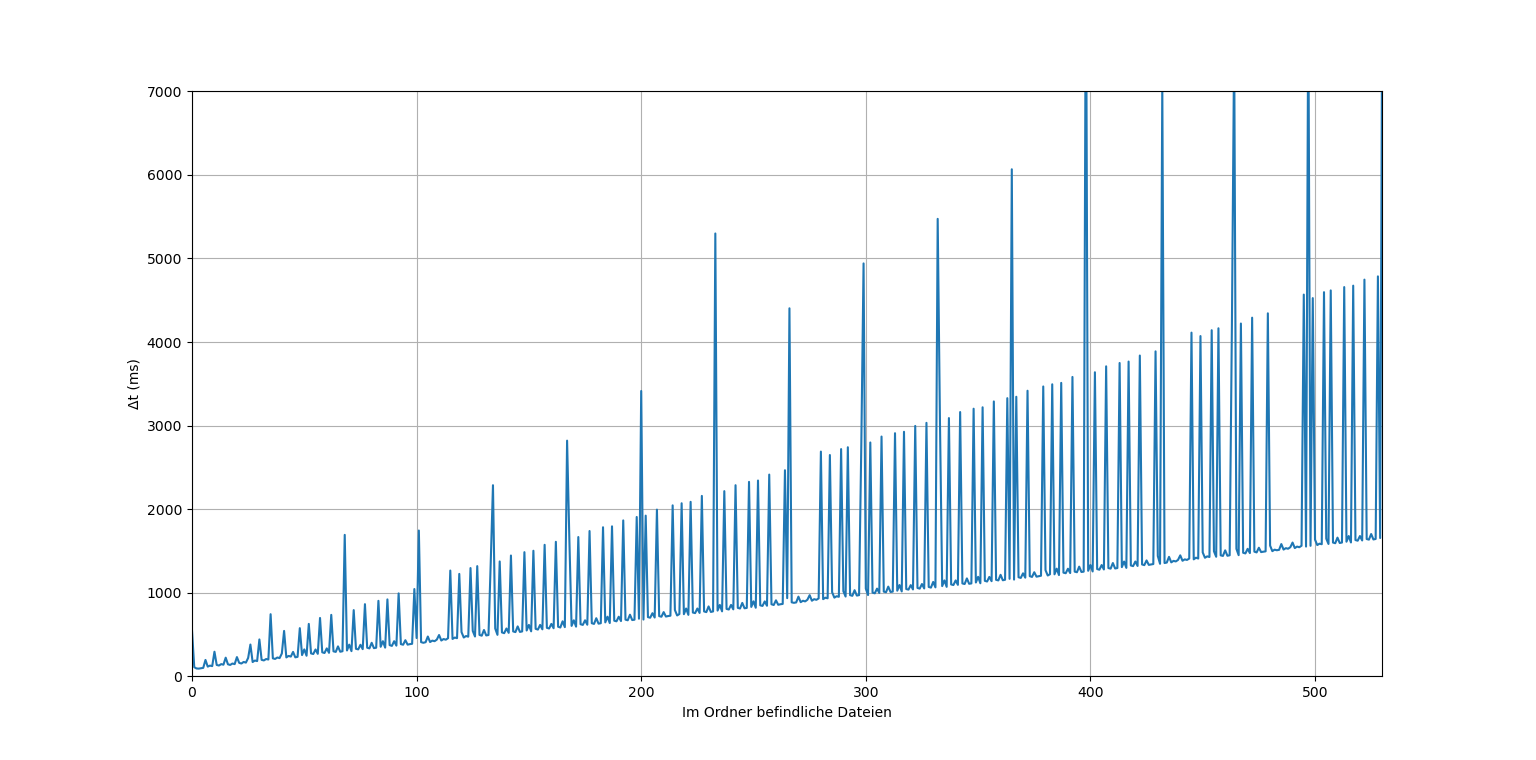
\includegraphics[width=\textwidth, trim=3cm 0cm 3cm 0cm, clip]{Bilder_Plot/3_WT2_littlefs_dateierstellzeit.png}
    \caption{Dauer der Neuerstellung von Dateien auf dem littlefs-Dateisystem mit korrupten Daten}
    \label{fig:littlefstime_corr}
\end{figure}

\fig{fig:littlefstime_corr} zeigt den aus Versuch 1 bekannten Graphen, in dem die Dauer gezeichnet wird,
die die Neuerstellung einer Datei in Abh"angigkeit von den sich bereits im Ordner befindlichen Dateien ben"otigt. 
Logischerweise ben"otigt littlefs viel h"aufiger l"angere Zeit zur Erstellung einer Datei als zuvor,
da es nach der Fehlerpr"ufung die Daten neu anfordern und neu senden muss.

Bei FatFs hingegen f"allt allein schon die automatische Auswertung schwer:
Durch Fehler sowohl beim Dateninhalt als auch in den Metadaten (Dateiname, Zeitstempel, Dateigr"o"se etc.)
l"asst sich das zuvor verwendete Skript nicht zuverl"assig anwenden.
Von 337 Dateien haben mindestens 28 Formatierungsfehler im Dateinamen, 8 Dateinamen sind dabei v"ollig unkenntlich.
66 Dateien haben jeweils exakt einen Schreibfehler im Inhalt. Zus"atzlich gab es Fehler bei der Dateigr"o"se und 
im Zeitstempel. Diese wurden leider beim Kopieren in den Testordner bereits wieder beseitigt, da sie beim Kopieren
auf ein neues Dateisystem "uberf"uhrt wurden.


\begin{figure}[H]
    \centering
    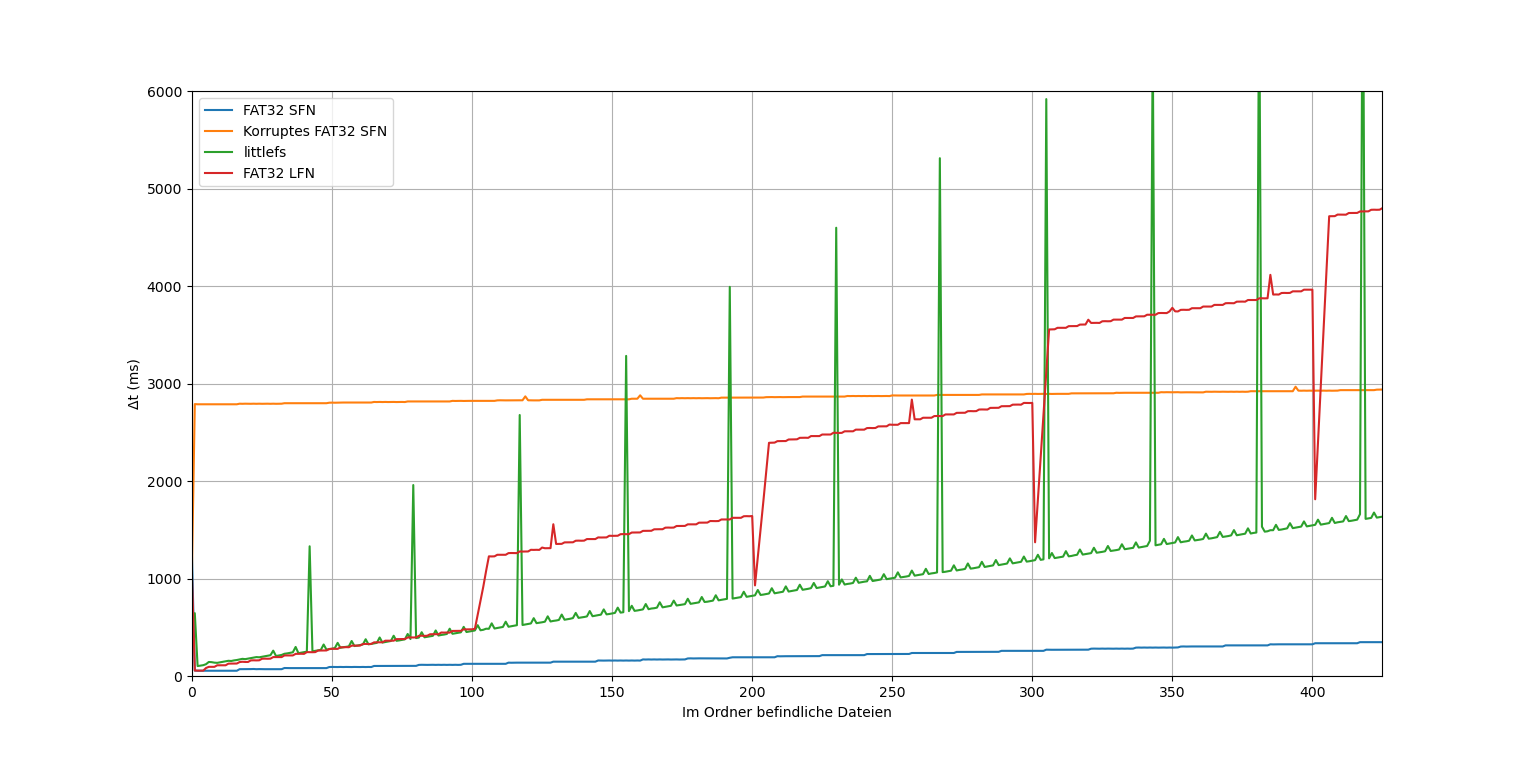
\includegraphics[width=\textwidth, trim=3cm 0cm 3cm 0cm, clip]{Bilder_Plot/4_dateierstellzeit_all.png}
    \caption{Dauer der Neuerstellung von 1\,KB Dateien "Ubersicht}
    \label{fig:dateierstellalle}
\end{figure}

\fig{fig:dateierstellalle} zeigt eine "Ubersicht "uber die Dateierstellzeiten in verschiedenen Kontexten.
Interessant ist hier der Graph f"ur \enquote{Korruptes FAT32 SFN}. Ein L"oschen der korrupten FAT32 Dateien
war hier nur bedingt m"oglich. Das zur"uckgebliebene inkonsistente Dateisystem hat verglichen mit 
einem frisch formatierten FAT32 erhebliche Performanceprobleme. An dieser Stelle sei erw"ahnt, dass alle Graphen
in \fig{fig:dateierstellalle} im Gegensatz zu \fig{fig:littlefstime_corr} mit einer unmanipulierten Schreibfunktion
erstellt wurden. Die Zeitverz"ogerung f"ur den Graphen \enquote{Korruptes FAT32 SFN} entsteht lediglich durch 
ein inkonsistentes Dateisystem. Dieses kann nur durch Neuformatierung oder
durch spezialisierte Software wie \enquote{fsck (file system check)} wieder repariert werden.  

\subsubsection*{Fazit Versuch 2}
Bei einem unsicheren "Ubertragungskanal f"ur die Daten bedarf es f"ur das FAT-Dateisystem einer gesonderten Strategie, 
um die Integrit"at der Daten und des Dateisystems zu sichern. Dies ist allerdings nicht trivial:
Wenn die Metadaten korrupt sind, so ist beispielsweise ein "Offnen der Datei mit der 
\texttt{fopen}-Funktion von FatFs gar nicht in allen F"allen m"oglich, 
da der Dateiname sich m"oglicherweise ver"andert hat. 
Deutlich einfacher scheint
die Einf"uhrung einer neuen, sicheren Schreibfunktion auf SD-Treiberebene,
die das Zur"ucklesen direkt "ubernimmt und im Zweifelsfall die Operation wiederholt.\\

Littlefs hingegen bringt durch die im Kapitel \hyperref[sec:funclittle]{Funktionsweise littlefs} 
besprochenen Schutzmechanismen hier klare Vorteile mit sich.



\subsection{Versuch 3: Analyse von pseudo-randomisierter Zeichenfolge bei Anhang an Datei}\label{sec:v3}
Die Idee dieses Versuches ist einerseits, die Konsistenz der Schreiboperationen
bei pseudo-zuf"alligen Daten festzustellen, andererseits die Schreibperformance
bei dem Anh"angen von Daten an eine bereits existierende Datei im Gegensatz zur Neuerstellung 
der Datei zu untersuchen. Weiterhin wurde der SPI-Takt bei diesem Versuch auf 8 MHz erh"oht,
um mehr potenzielle Schreibfehler zu provozieren.\\


\begin{figure}[H]
    \centering
    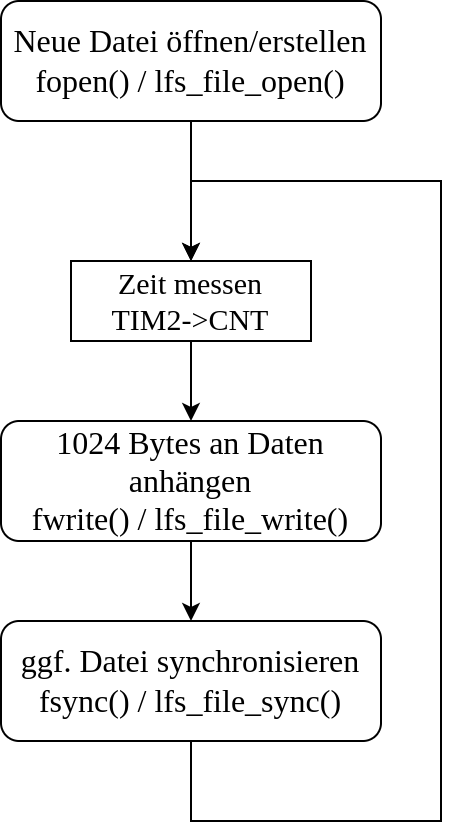
\includegraphics[height=8cm]{Bilder_Diagramme/Versuch3loop.png}
    \caption{Schleife f"ur das Anh"angen von 1024 Byte an eine Versuchsdatei}
    \label{fig:versuch3loop}
\end{figure}

Bisher wurde prim"ar die Neuerstellung von kleinen Dateien der Gr"o"se 1 KB untersucht.
Es wurde in den vorherigen Versuchen festgestellt, 
dass der Zeitaufwand der Neuerstellung einer Datei bei
beiden Dateisystemen linear zunimmt. F"ur die dauerhafte Aufnahme von Daten ist das sehr nachteilhaft:
F"ur eine Echtzeitgarantie bei der Aufnahme von Daten 
m"usste die Anzahl der bereits im Ordner befindlichen Dateien berücksichtigt werden 
und gegebenenfalls ein neuer Ordner erstellt werden.
Daher wurde mit den Tests \texttt{test/fatfs\_append\_write\_test.cpp} und 
\texttt{test/littlefs\_append\_write\_test.cpp} die Zeitdauer aufgenommen, die das Anh"angen
von 1\,KB Daten an eine bestehende Datei ben"otigt.

\begin{figure}[H]
    \centering
    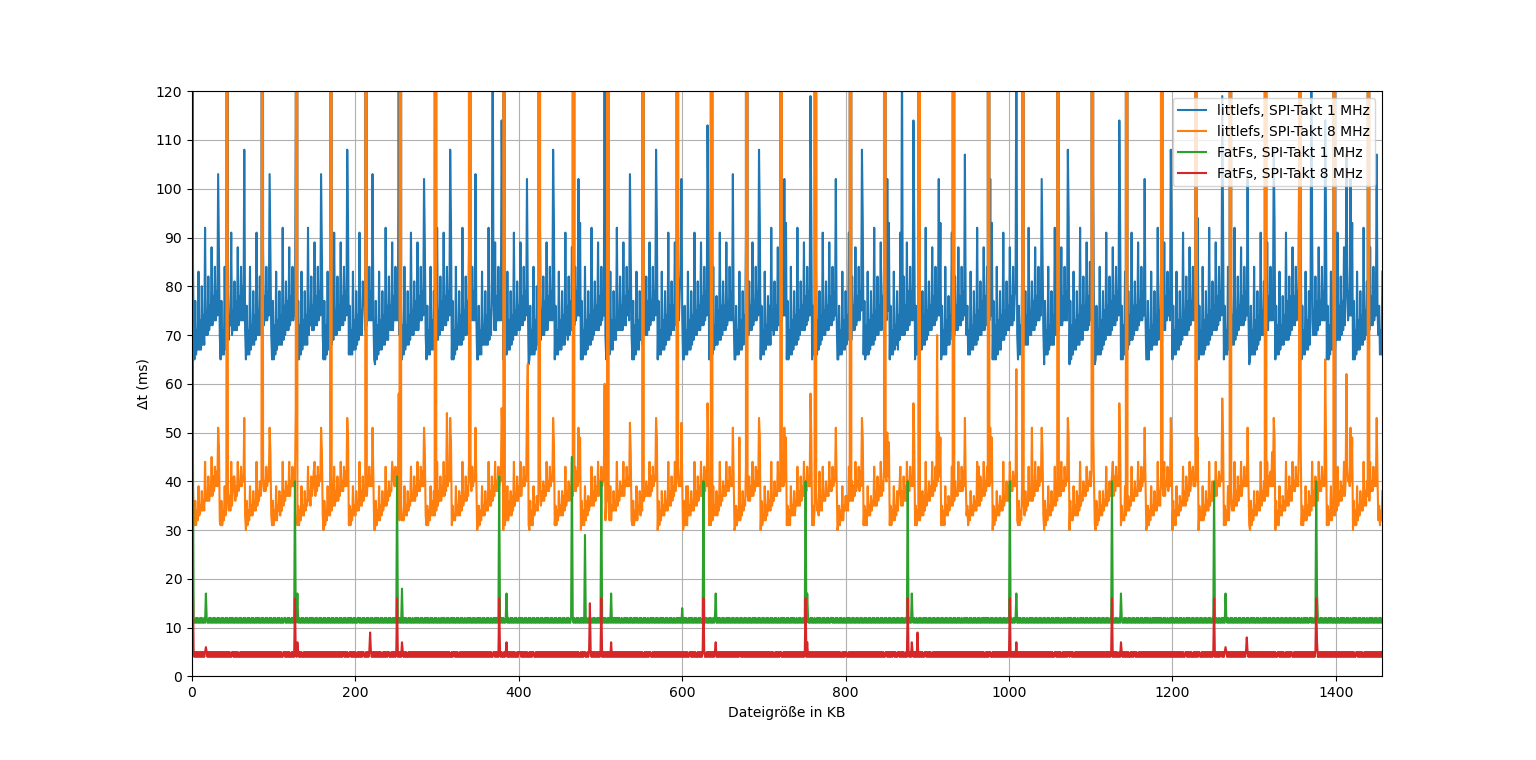
\includegraphics[width=\textwidth, trim=3cm 0cm 3cm 0cm, clip]{Bilder_Plot/6_WT3_zeitenzoomin.png}
    \caption{Dauer des Anh"angens von 1\,KB an eine Datei in Abh"angigkeit der Dateigr"o"se}
    \label{fig:timeappend2}
\end{figure}


\begin{figure}[H]
    \centering
    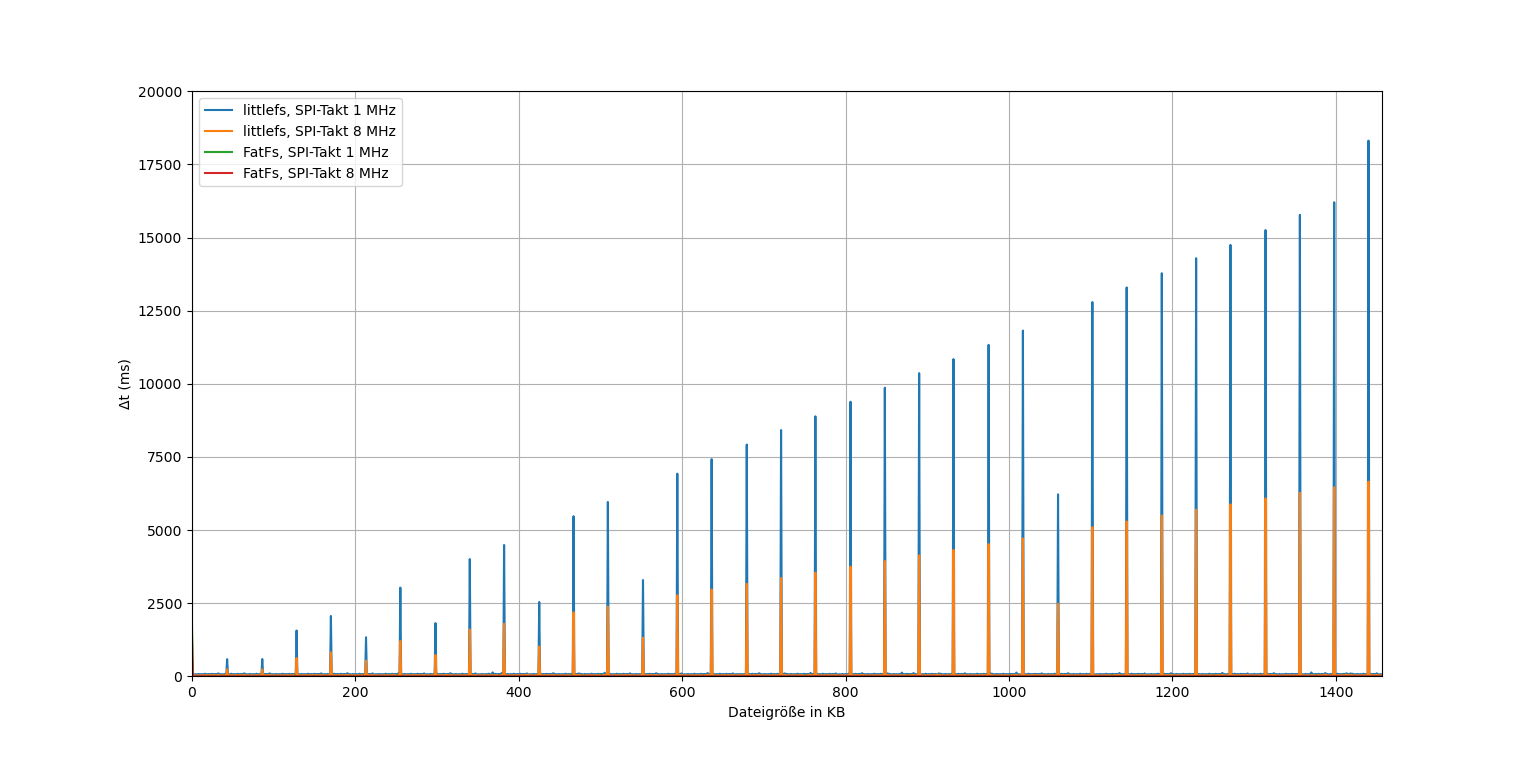
\includegraphics[width=\textwidth, trim=3cm 0cm 3cm 0cm, clip]{Bilder_Plot/5_WT3_zeitenzoomout.png}
    \caption{Dauer des Anh"angens von 1\,KB an eine Datei in Abh"angigkeit der Dateigr"o"se}
    \label{fig:timeappend1}
\end{figure}



\Fig{fig:timeappend2} und \ref{fig:timeappend1} zeigen anschaulich das Verhalten der beiden Dateisysteme und
nutzen denselben Datensatz in unterschiedlicher Skalierung.
W"ahrend das Anh"angen von 1 KB Datengr"o"se an eine Datei bei FatFs eine sehr gute, konstante Performance
von 5\,ms bei 8\,MHz liefert, zeigt sich bei littlefs der Overhead der Datenintegrit"atskontrolle: 
Grunds"atzlich ist der Schreibzyklus beim littlefs-Dateisystem ca. 8-mal langsamer. 
Das weitaus problematischere Verhalten ist aber, dass das Anh"angen von Daten in regelm"a"sigen Abst"anden deutlich
l"anger braucht. Die zus"atzliche Zeit, die es ben"otigt, ist abh"angig von der Dateigr"o"se.
Bei einer Dateigr"o"se von nur 1 MB dauert diese zus"atzliche Erstellzeit bereits "uber 10\s.
Eine bessere Implementierung und gr"o"sere Buffer in der Konfiguration k"onnen diese Zahlen quantitativ
zwar reduzieren, "andern aber nichts an ihrem prinzipiellen Vorhandensein. 
Das macht littlefs als Echtzeitdateisystem unbrauchbar. Im Hintergrund scheint littlefs f"ur seine
Dateiintegrit"atsmechanismen immer wieder die gesamte Datei zu "uberpr"ufen, was f"ur einen Einsatz 
in embedded Umgebungen zu viele Hardwareressourcen bindet. Dateisysteme wie ext4 nutzen ihr Journaling
beispielsweise bewusst nur f"ur ihre Metadaten, 
um die Dateisystemintegrit"at abzusichern, damit es nicht zu schweren Performanceeinbu"sen kommt wie
sie hier zu beobachten sind.\\

 





\subsubsection*{Fazit Versuch 3}
Die Schutzmechanismen von littlefs konnten in diesem Versuch ihre Funktionalit"at beweisen.
Gleichzeitig wurde aber auch ein Performanceproblem beobachtet, das f"ur den 
Einsatz in einem praktischen System zun"achst einmal gel"ost werden m"usste. \\
FatFs hingegen gestaltet sich wie erwartet bei unsicherem Daten"ubertragungskanal 
nicht resilient gegen"uber Fehlern und f"uhrt zu potenziell schweren Datei- und Dateisysteminkonsistenzen.





\subsection{Versuch 4: Verhalten der Dateisysteme bei Stromunterbrechungen}\label{sec:v4}
Die Entwickler des littlefs-Dateisystems versprechen
eine hohe Datei- und Dateisystemkonsistenz bei Stromausf"allen. Dies soll
praktisch getestet werden und mit dem FAT-Dateisystem verglichen werden.
Eine erste Idee war, die \texttt{Watchdog}-Funktionalit"at des STM32G431 zu nutzen.
Diese greift allerdings zu kurz, da dabei keine Unterbrechung der SD-Karten-Spannungsversorgung
herbeigef"uhrt wird.\\
Die Spannungsversorgung der in dieser Bachelorarbeit verwendeten Platine wird entweder "uber die vorhandene 5\,V USB-C-Buchse
oder "uber eine Stiftleiste, die haupts"achlich f"ur
ein Batteriefach mit einer variablen Spannung zwischen 3,8\,V und 5,5\,V gedacht ist, gew"ahrleistet. Welche der
beiden Optionen verwendet wird, entscheidet ein Jumper. An dieser Stelle l"asst sich praktischerweise
eine externe Schaltung einklinken, die periodisch die Spannungsversorgung unterbricht. 

\begin{figure}[H]
    \centering
    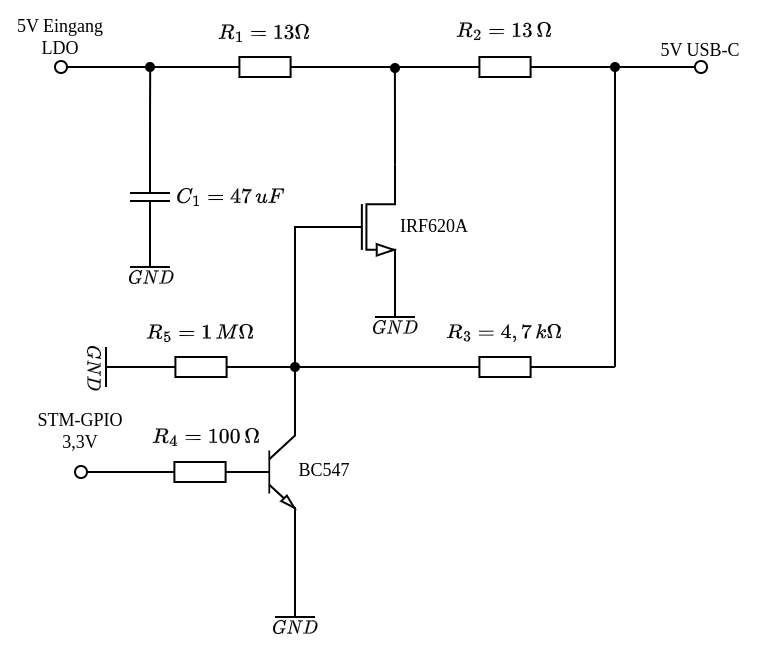
\includegraphics[height=12cm]{Bilder_Diagramme/killswitchschaltung.png}
    \caption{\enquote{killswitch}-Schaltung f"ur eine periodische Unterbrechung der Spannungsversorgung}
    \label{fig:killswitch}
\end{figure}



\fig{fig:killswitch} zeigt die f"ur diesen Versuch erstellte Schaltung. Leider musste diese
aufgrund der vorhandenen Bauteile etwas komplexer gestaltet werden als im Prinzip notwendig.
Letztlich wird lediglich ein Schalter ben"otigt, der periodisch 5\,V an- und ausschaltet.
So w"are ein mit 3,3 V schaltbares Relais mit einer R"ucklaufdiode ausreichend f"ur diesen Zweck gewesen.
Aufgrund von eingeschr"ankter Bauteilverf"ugbarkeit wurde aber auf den vorhandenen MOSFET \texttt{IRF620A} zur"uckgegriffen.
Dieser kann im durchgeschalteten Zustand den Pegel vom 5\,V LDO Eingang auf nahezu 0 V bringen. Das ist ohne destruktiven Kurzschluss
nat"urlich nur durch die Widerst"ande $R_1$ und $R_2$ m"oglich. Diese begrenzen den f"ur den LDO verf"ugbaren Strom auf
rund $\frac{5\,V}{26\,\Omega} \approx 190\,mA$. Dies ist f"ur die durchschnittliche Stromaufnahme der Platine (gemessen: 23,3\,mA)
vollkommen ausreichend und wird mit dem Kondensator $C_1$ zus"atzlich gepuffert. 
Gleichzeitig kann der verwendete MOSFET den Stromfluss problemlos gegen GND abf"uhren, sodass die Spannung
auf 0\,V einbricht. Unter der Annahme, dass der MOSFET im durchgeschalteten Zustand keinen Innenwiderstand besitzt, flie"st einerseits
ein Strom von $\frac{5\,V}{13\,\Omega} \approx 385\,mA$ vom USB-C Zweig, 
andererseits ebenfalls maximal 385\,mA vom Zweig mit dem Kondensator $C_1$.
Da der MOSFET bis zu 5\,A schalten kann, ist dies im sicheren Bereich f"ur das Bauteil. \\
\begin{figure}[H]
    \centering
    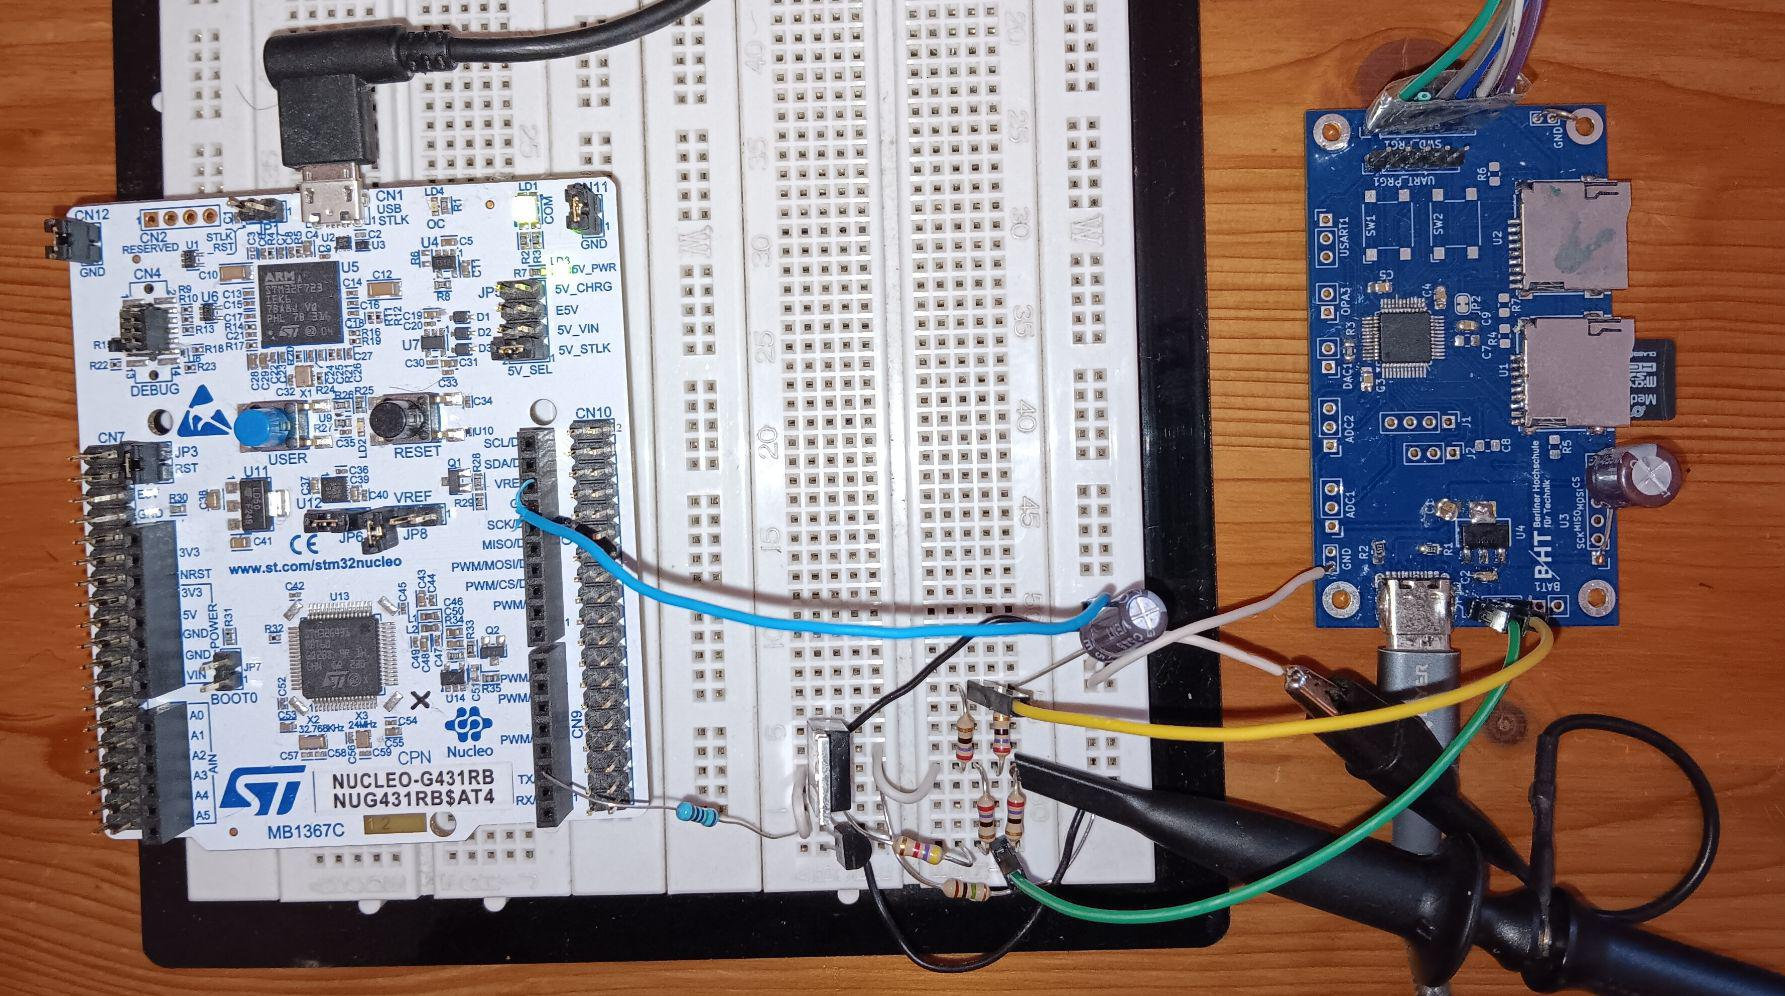
\includegraphics[height=8cm]{Hard_Bilder/killswitchsteckbrett.jpg}
    \caption{Aufbau der \enquote{killswitch}-Schaltung auf einem Steckbrett}
    \label{fig:killswitchaufbau}
\end{figure}
Die Idee war zun"achst, den MOSFET mit einem GPIO-Pin eines externen Nucleo-Boards zu schalten. Leider schaltet 
der \texttt{IRF620A} erst zuverl"assig bei $U_{gs}=5\,\mathrm{V}$ durch, sodass ein zus"atzlicher NPN-Transistor in Emitterschaltung
hinzugef"ugt werden musste, der die 5\,V der USB-C Buchse nutzt. Dieser kann dann mit dem GPIO-Pin eines beliebigen Nucleo-Boards geschaltet
werden.


\begin{listing}[H]
    \begin{minted}[
        frame=lines,      % Rahmenlinien oben und unten
        framesep=2mm,     % Abstand zum Rahmen
        baselinestretch=1.2,
        bgcolor=lightgray!20, % Hintergrundfarbe
        fontsize=\footnotesize,
        linenos           % Zeilennummern aktivieren
    ]{cpp}
    GPIO_Init();
    TIM2_Init();

    GpioPin<GPIOA_BASE,10>::OutputInit(Level::High);
    for(;;)
    {
        //ON for 10 secs
        GpioPin<GPIOA_BASE,10>::setHigh();
        delay_s<10>();
        //OFF for 3 secs
        GpioPin<GPIOA_BASE,10>::setLow();
        delay_s<3>();
    }
    \end{minted}
\caption{Hauptschleife aus Datei \texttt{src/killswitch.cpp}}
\label{listing:killswitchcode}
\end{listing}
\coderef{listing:killswitchcode} zeigt praktisch den gesamten Quelltext der Datei \text{src/killswitch.cpp},
der aufgrund der bereits vorhandenen Abstraktionen sehr einfach ausf"allt. F"ur 10\,s bleibt
der GPIO-Pin auf einem 3,3\,V Pegel und erlaubt der Dateisystem-Platine den Schreibtest auszuf"uhren.
Dann wird der Pin auf einen 0\,V Pegel gesetzt und simuliert der Platine einen pl"otzlichen Stromausfall.
Es finden in diesem Versuch also ca. 4 Stromausf"alle pro Minute statt.


\begin{figure}[H]
    \centering
    \includegraphics[width=\textwidth]{Bilder/stm-killswitch.png}
    \caption{Verifizierung der Spannung am LDO-Eingang}
    \label{fig:killswitchoszi}
\end{figure}

\fig{fig:killswitchoszi} verifiziert die korrekte Spannungsversorgung am LDO-Eingang. 
Es f"allt zus"atzlich auf, dass die Schaltung etwas Rauschen eingebracht hat, was f"ur diesen Versuch,
der Schreibfehler provozieren soll, grunds"atzlich positiv zu bewerten ist. \\

Die verwendeten Programme f"ur den Test sind \texttt{test/fatfs\_killswitch\_test.cpp} \\
und \texttt{test/littlefs\_killswitch\_test.cpp}. Der Test an sich nutzt wieder eine f"ur
Menschen lesbare, verifizierbare Zeichenfolge. Diese ist bei Fehlern leichter handzuhaben als die
pseudo-randomisierte Folge aus dem vorherigen Versuch. 
Das Programm pr"uft zun"achst, wie viele Testdateien bereits existieren und erstellt
dann die n"achstgr"o"sere Datei.
Grunds"atzlich wird dann eine bekannte Zeichenfolge
bis zum Stromausfall an die erstellte Datei immer wieder angeh"angt.
Die Gr"o"se der Dateien h"angt also haupts"achlich davon ab, wie schnell die
Dateisysteme den n"achsten freien Dateinamen finden und wie schnell sie an
diese Datei anh"angen k"onnen.\\
Die SPI-Clock wurde auf das maximale Tempo von 8 MHz gesetzt.
Es wurden f"ur diesen Test rund 140\,MB FatFs-Daten und 2,1\,MB an littlefs-Daten erzeugt.
Die verh"altnism"a"sig geringe Menge an littlefs-Daten h"angt damit zusammen,
dass das Dateisystem auch beim Suchen der Dateien deutlich langsamer ist als FatFs und es somit
innerhalb der vorgegebenen 10 Sekunden Versuchslaufzeit maximal 52 Dateien erstellen konnte.
Alle weiteren Versuche beanspruchen schlichtweg mehr als 10 Sekunden f"ur die Suche des n"achsten
freien Dateinamens und die Erstellung einer neuen Datei. Der Algorithmus lie"se sich nat"urlich
optimieren, sodass noch mehr littlefs-Testdaten erzeugt werden k"onnen. Tats"achlich zeigen allerdings
die Testdaten des unsichereren Dateisystems FatFs, dass sich mit Stromausf"allen auf SD-Karten 
praktisch keine Schreibfehler erzeugen lassen. \\
Der Effekt war bei FatFs im "Ubrigen ebenfalls vorhanden.
Dennoch konnte problemlos die 70-fache Menge an Daten in derselben Zeit erzeugt werden. 
Das Pythonskript zur Verifikation findet sich unter 
\href{https://github.com/miko8278/stm32-SPI-SD-card/tree/main/test\_data/Writetest4/test\_readable.py}{(root)/test\_data/Writetest4/test\_readable.py}.

\subsubsection*{Fazit Versuch 4}
Trotz der kontinuierlichen Stromausf"alle kam es in keinem der beiden Dateisysteme auch nur zu einem Schreibfehler.
In Kombination mit den vorangegangenen Versuchen l"asst sich somit behaupten,
dass Schreibfehler im "ublichen SD-Kartenbetrieb sehr selten sind und selbst bei exzessiven Stromausf"allen
nicht h"aufig vorkommen:
Nach der statistischen Dreier-Regel (Rule of Three) lässt sich 
bei $N$ fehlerfreien Übertragungen die maximale Bitfehlerrate (BER) 
für eine Sicherheit von 95\,\% wie folgt grob absch"atzen:
$$
\text{BER}_{95\%} \le \frac{3}{N}
$$

\noindent
Aufgrund von 140 MB an fehlerfreien Daten folgt dann $N=140\cdot1024\cdot1024\cdot8$ Bits.

$$
\text{BER}_{95\%} \le \frac{3}{140\cdot1024\cdot1024\cdot8} \approx 2{,}55 \cdot 10^{-9}
$$

Der Versuch sch"atzt also eine maximale Bitfehlerrate in der Gr"o"senordnung von $10^{-9}$ bei
exzessiven Stromausf"allen und fehlender CRC-Pr"ufsumme auf SD-"Ubertragungsebene. Der 
in die Karte integrierte SD-Kartencontroller scheint also bereits daf"ur zu sorgen,
dass auch bei Stromausf"allen nur verl"assliche Daten auf der Karte landen. F"ur eine
zus"atzliche Sicherheit bei der "Ubertragung lie"se sich die CRC-Pr"ufsumme, die im SPI-Modus
standardm"a"sig deaktiviert ist, wieder aktivieren.\\

Der Versuch hat ebenfalls noch einmal verdeutlicht, dass der Umgang mit littlefs 
in Echtzeitsystemen sehr genau geplant sein muss. F"ur eine Einhaltung von gegebenen Zeitgrenzen m"ussen
bei dem Dateisystem vorab Tests und Messungen gemacht werden, w"ahrend FatFs sich responsiver und weniger
unberechenbar verh"alt.\\

Das endg"ultige Fazit ist, dass der zus"atzliche Datenschutz durch das littlefs-Dateisystem die h"ohere Komplexit"at
des Systems im Zusammenhang mit SD-Karten nicht rechtfertigt. In anderen Anwendungen, vor allem bei einem gegebenen unsicheren Datenkanal,
ist littlefs durchaus erw"agenswert. 

\subsection{Versuch 5: Direkte Blockadressierung (NoFs)}\label{sec:v5}
Die vorangegangenen Kapitel untersuchten das Verhalten von littlefs und FatFs in unterschiedlichen Szenarien.
Angedacht war auch die Untersuchung von direkter Blockadressierung. Dies hat sich aber aus mehreren Gr"unden
als nicht sinnvoll herausgestellt: Einerseits nutzen beide Dateisysteme die Funktionen der Blockadressierung 
als Basis.
Wenn es FatFs m"oglich ist, fehlerfrei Dateien zu erstellen, so pr"uft das indirekt ein korrektes
Verhalten der SD-Kartenblockschreibfunktionen. \\
Andererseits ist der Aufwand nicht ganz unerheblich: W"ahrend FatFs und littlefs im Prinzip "ahnliche
Funktionen zum "Offnen, Schreiben und Schlie"sen bereitstellen, so muss f"ur die direkte
Blockadressierung eine eigene Struktur erfunden werden, in der die Daten abgelegt werden.
Ein ganz direkter Vergleich ist damit auch nicht m"oglich. \\
Am ehesten l"asst sich Teil 1 von \hyperref[sec:v3]{Versuch 3} wiederholen, der die 
Zeitdauer des Dateianhangs von 1\,KB Daten misst. Das ist insofern inhaltlich interessant,
weil es aufzeigt, wie viel Zeit das eigentliche Schreiben von Bl"ocken mit den gegebenen Funktionen ben"otigt
und wie viel Zeit dem Overhead des Dateisystems zuzuordnen ist. \\ 

Gemessen wird die Dauer f"ur das Schreiben eines Blocks (512 Bytes) und die Dauer des Schreibens
f"ur zwei Bl"ocke (1024 Bytes). Das Schreiben von mehreren Bl"ocken nutzt ein unterschiedliches
SD-Kommando und sollte zeitm"a"sig dem Schreiben von einzelnen Bl"ocken "uberlegen sein.  
Auf einem Linuxsystem lassen sich die Rohdaten wiederum mit \\
\mintinline[]{bash}|dd if=/dev/sdx of=sd_karte_dump.bin bs=512 count=Anzahl_Bloecke status=progress|
extrahieren.\\
Die Versuchsquelldateien finden sich in \texttt{test/nofs\_append\_write\_test\_512.cpp} und \\
\texttt{test/nofs\_append\_write\_test\_1024.cpp}. \\
Die aufgenommenen Testdaten sind unter
\href{https://github.com/miko8278/stm32-SPI-SD-card/tree/main/test_data/Writetest5}{(root)/test\_data/Writetest5} erreichbar.
Der SPI-Clock wurde bei 1 MHz belassen.



\begin{figure}[H]
    \centering
    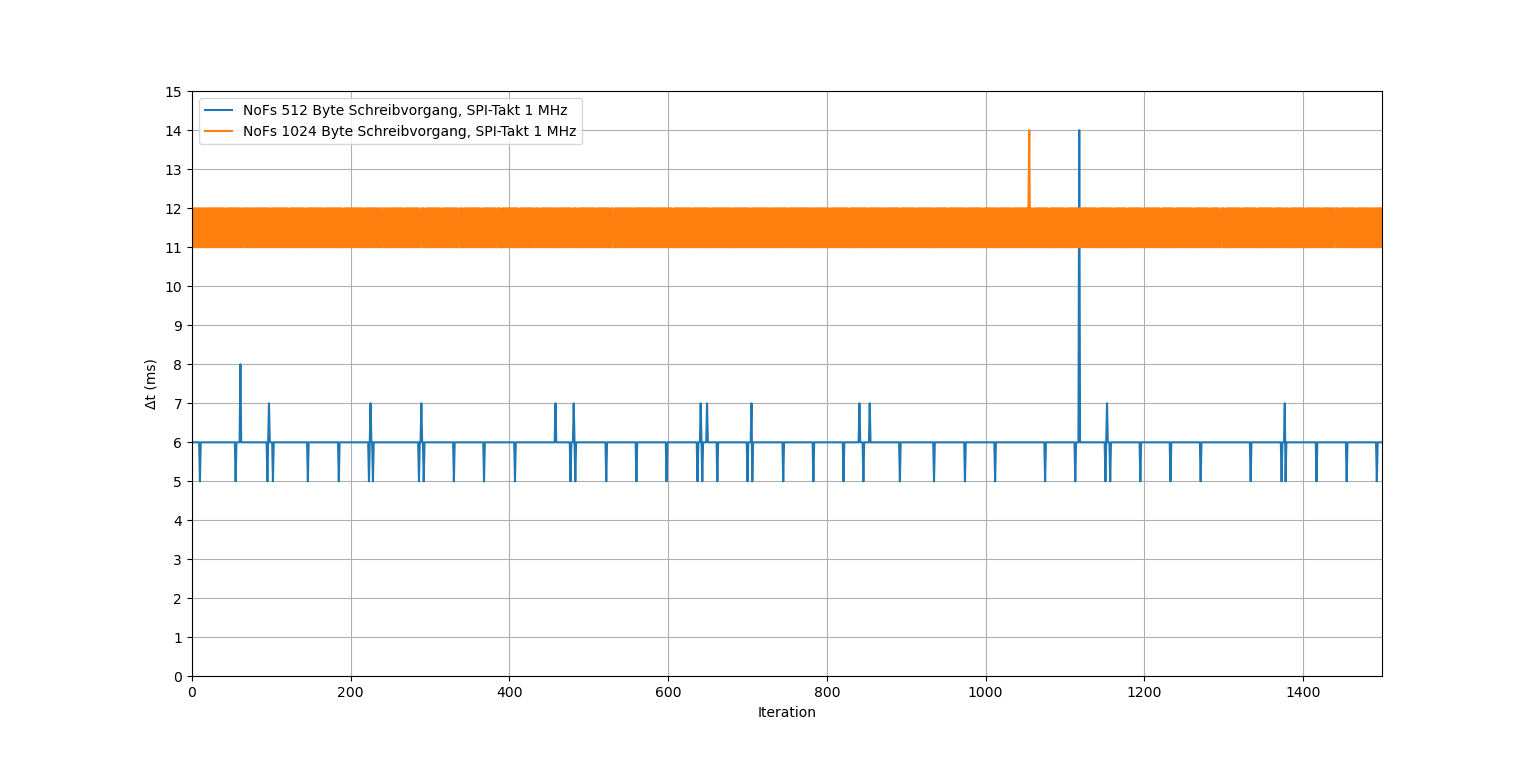
\includegraphics[width=\textwidth, trim=3cm 0cm 3cm 0cm, clip]{Bilder_Diagramme/NoFs_time.png}
    \caption{Dauer von 512 Byte und 1024 Byte Schreibvorg"angen}
    \label{fig:nofstime}
\end{figure}

\fig{fig:nofstime} plottet die aufgenommenen Daten. Dabei war bereits zu erwarten, dass das Schreiben
eines 512 Byte Blocks in etwa doppelt so lange in Anspruch nimmt wie das Schreiben von zwei 512 Byte
Bl"ocken.
\tab{tab:schreibdauer} nimmt den Durchschnitt der ersten 1000 Werte f"ur die Schreibdauer
von 1024 Bytes. F"ur NoFs (Einzelblock) wurde die aufgenommene Dauer verdoppelt.
Interessant ist hierbei auch ein Vergleich der Daten von littlefs (SPI 1\,MHz) und FatFs (SPI 1\,MHz) aus \hyperref[sec:v3]{Versuch 3}.
Tats"achlich zeigt sich, dass FatFs in seiner Performance sogar besser abschneidet als 
NoFs bei Nutzung der Einzelblockschreibfunktion. Es f"uhrt beim Anh"angen an eine Datei
im Prinzip gar keinen Schreibzeitoverhead ein. Der Unterschied zwischen dem Schreiben
von zwei Bl"ocken und dem Schreiben von einem Einzelblock betr"agt lediglich 0,5 ms.
Dieser w"urde aller Voraussicht nach beim Schreiben von noch mehr Bl"ocken gleichzeitig
mehr ins Gewicht fallen. Dadurch, dass in den allermeisten F"allen die zu schreibenden Informationen
in einen Schreibbuffer gelegt werden m"ussen, k"onnen in ressourcenbeschränkten Umgebungen
aber nicht beliebig viele Bl"ocke gleichzeitig geschrieben werden. \\
\begin{table}[H]
    \centering
    \caption{Durchschnittliche Dauer des Schreibvorgangs für 1024 Bytes}
    \label{tab:schreibdauer}
    \begin{tabular}{lcc}
        \hline
        \textbf{Dateisystem} & \textbf{$\Delta$t 1024 Bytes} & Datenrate  \\
        \hline
        NoFs (Einzelblock)  & 11,96\,ms & 85618,72 B/s\\
        NoFs (Multiblock)  & 11,48\,ms & 89198,61 B/s\\
        FatFs SFN           & 11,74\,ms & 87223,17 B/s\\
        littlefs            & 202\,ms & 5069,31 B/s\\
        \hline
    \end{tabular}
\end{table}
Zeitm"a"sig deutlich schlechter schneidet littlefs ab, wobei die Durchschnittsbildung in diesem Fall etwas irref"uhrend ist:
Grunds"atzlich dauert das Anh"angen von 1\,KB bei littlefs um die 80\,ms. Der Durchschnitt wird
aber durch extreme Ausrei"ser, die mehrere Sekunden dauern k"onnen, stark gesenkt. \\
Die ideale Datenrate bei dem verwendeten SPI-Takt von 1\,MHz betr"agt 125000\,B/s. In allen F"allen ist beim Design
die Erstellung des 1024 Byte Datenbuffers mitgemessen worden, sodass die eigentliche Datenrate sogar ein
klein wenig h"oher ausf"allt. Zudem muss bedacht werden, dass hier lediglich die Geschwindigkeit des Payloads gemessen
wurde. Das SD-Protokoll selbst hat einen Overhead f"ur die SD-Kommandos, zus"atzlich entstehen teilweise 
Wartezeiten, weil die SD-Karte noch vorangegangene Operationen zu Ende f"uhren muss. \\ 
FatFs und NoFs befinden sich in ihrer Schreibperformance also erstaunlich nah 
am physikalischen Limit der SPI-Peripherie. 

\subsubsection*{Fazit Versuch 5}
Das Fazit in diesem Versuch ist die Erkenntnis, dass FatFs bei der genutzten Konfiguration und
den vorhandenen Blockschreibfunktionen keinen Schreiboverhead einf"uhrt. Da bereits festgestellt wurde,
dass FatFs auch hinsichtlich der RAM-Nutzung kaum schwerer wiegt als NoFs, ist der einzige gr"o"sere Nachteil
von FatFs gegen"uber NoFs der Flashverbrauch, der im schlimmsten Fall rund 13\,KB h"oher ausf"allt. 

\section{Gesamtfazit}

Die Hardware war f"ur einen ersten Prototypen gut geeignet und funktional. Alle Schreib-
und Leseversuche lie"sen sich damit zun"achst einmal durchf"uhren. F"ur zuk"unftige 
Produkte m"usste der beschriebene Spannungseinbruch in der MISO-Leitung bei einer der zwei SPI-Peripherien
n"aher untersucht werden. \\
Auf der Softwareseite hat sich das Setup aus CMake, VS Code, Cortex-Debug und C++ bew"ahrt:
Dank CMake konnten bei "Anderungen in den Hauptquelldateien zahlreiche Binaries zur selben
Zeit automatisiert kompiliert werden. Da das System nur ver"anderte Dateien kompiliert, war die 
Kompilierzeit sehr niedrig und die Iterationsgeschwindigkeit f"ur neue Funktionen sehr hoch.
W"ahrend die weitaus komplexere Syntax von C++ im Vergleich zu C abschreckend ist,
bieten moderne Funktionalit"aten mehr M"oglichkeiten Abstraktion, Wiederverwendbarkeit
und Erweiterbarkeit f"ur zuk"unftige Projekte. Da viel Abstraktion mit modernem C++ in
die Kompilierzeit verschoben werden kann, bleibt die Ausf"uhrungsgeschwindigkeit trotz
Nutzung von (eigenen) Libraries wie der \texttt{src/GPIO\_HAL.hpp} sehr hoch.\\
Die Arbeit am SD-Treiber war eine
der Grundvoraussetzungen f"ur den Rest der Arbeit. Nat"urlich implementiert diese nicht 
das gesamte SD-Protokoll, sondern nur die f"ur diese Arbeit relevanten Funktionen:
Das Schreiben und Lesen von Einzel- und Mehrfachbl"ocken und das Abrufen von SD-Karteninformationen.
Es konnte festgestellt werden, dass die Schreibperformance sich nah an der physikalischen Grenze 
der SPI-Peripherie befindet und sehr zuverl"assig funktioniert. Tats"achlich lie"s sich "uber 
alle Versuche hinweg kein einziger Schreibfehler provozieren und es musste f"ur eine Untersuchung
von Schreibfehlern eine gezielte Injektion von falschen Daten erfolgen.\\ 
Ein weiterer Vorteil des SD-Treibers ist der recht geringe Flashspeicherverbrauch von nur rund 2\,KB,
sodass er sich problemlos in eine Vielzahl von weiteren aufbauenden Projekten integrieren l"asst.
Ein gro"ser Teil der Arbeit bestand in dem Vergleich zwischen FatFs und littlefs.
Noch einmal sollen an dieser Stelle die drei gro"sen Vorteile des littlefs-Dateisystems genannt werden:
\begin{itemize}
    \item \textbf{Ausfallsicherheit bei Stromausfall} 
    \item \textbf{Verschleißregulierung des Flashspeichers (Wear Leveling)} 
    \item \textbf{Begrenzter RAM/ROM-Bedarf}
\end{itemize}

Leider fallen im Zusammenhang mit SD-Karten die Vorteile sehr gering aus:
\hyperref[sec:v4]{Versuch 4} hat gezeigt, dass die tats"achlichen Bitfehlerraten beim Schreiben und
der "Ubertragung extrem niedrig sind. Durch Nutzung der SD-karteninternen CRC-Pr"ufsumme besteht optional 
bereits auf SPI/SD-Kartenebene ein zus"atzlicher Fehlerschutz.
Gleichzeitig f"uhrt das integrierte Fehlerpr"ufsystem zu
einem Verlust von leicht vorhersagbarer Echtzeitf"ahigkeit des Systems, da das
Dateisystem in regelm"a"sigen Abst"anden deutlich l"anger zum Schreiben einer Datei braucht
als im Durchschnitt. \\
Verschleißregulierung des Flashspeichers ist hinf"allig, da der SD-Kartencontroller diese Aufgabe
bereits erledigt. W"ahrend dies in langen experimentellen Reihen getestet werden m"usste, bietet
die zus"atzliche Verschlei"sregulierung auf Dateisystemebene wahrscheinlich keine zus"atzlichen
positiven Effekte. Vielmehr scheint es wahrscheinlich, dass das zus"atzliche Journaling zu mehr
Schreiboperationen f"uhrt und damit potenziell die SD-Karte belastet. \\
Auch beim begrenzten RAM/ROM-Bedarf verliert littlefs im direkten Vergleich mit FatFs aufgrund seines 
komplexeren Aufbaus. Abschnitt \ref{sec:ramflash} zeigt die Gr"o"senunterschiede auf. W"ahrend 
littlefs sich vom Speicher her problemlos auf moderne Mikrocontroller programmieren l"asst, 
hat FatFs in einer gew"ohnlichen Standardkonfiguration lediglich die halbe Programmgr"o"se und l"asst
sich durch die Einschr"ankung von Optionen in der \texttt{FatFs/ffconf.h} sogar noch weiter verkleinern.\\
Dennoch hat \hyperref[sec:v2]{Versuch 2} klargemacht, dass die Verwendung von littlefs bei fehlerbehaftetem 
Datentragungskanal durchaus von Vorteil sein kann, wenn man die erw"ahnten Nachteile beachtet:
W"ahrend FatFs schnell zu Inkonsistenzen im Dateisystem, Metadaten und Dateien selbst neigt, demonstriert
littlefs eindrucksvoll, dass die Mechanismen zur Erkennung von fehlerhaften Daten selbst bei 
hohen Bitfehlerraten einwandfrei funktionieren.\\
Alles in allem gewinnt in der Praxis allerdings die Verwendung von FatFs bei SD-Karteneinsatz, selbst wenn 
es auf Datenintegrit"at ankommt:
Da das FAT-Dateisystem seit "uber 40 Jahren in Verwendung ist, existiert sehr viel Software wie 
beispielsweise \enquote{fsck}, die fehlerhafte Dateisystem- und Datenintegrit"at teilweise wiederherstellen kann.
Auch wenn es in dieser Arbeit nicht demonstriert wurde, so l"asst sich mit CRC-Pr"ufsummen auf SPI/SD-Kartenebene ohne einen erheblichen
Mehraufwand zus"atzliche Sicherungsschicht einf"uhren, die im Gegensatz zu littlefs die Schreibgeschwindigkeit weiterhin 
mit konstanter Laufzeit beibeh"alt. 
Fehlerschutz muss weiterhin nicht auf Dateisystemebene passieren: Aufbauend auf FatFs lassen sich externe Schutzmechanismen
wie die bereits genannten CRC-Pr"ufsummen oder kryptographische Hashfunktionen wie SHA-256 oder MD5 anwenden,
wie sie auch bei Downloads von gr"o"seren Dateien "ublich sind. Mit Datensicherungsstrategien wie doppelter oder dreifacher
Redundanz l"asst sich ohne zus"atzlichen Rechenaufwand zus"atzliche Sicherheit schaffen auf Kosten des Speicherplatzes.     
Die Verwendung von reinem Blockspeicher hingegen (NoFs) hat sich recht schnell als zu aufwendig herausgestellt:
Ohne die Herstellung eines eigenen Systems zur Speicherung der Daten ist das Wiederauffinden einer bestimmten
Information sehr schwierig. Weiterhin m"usste ein Mechanismus implementiert werden, der die Daten extrahiert
und letztlich wieder in eine dateisystemlesbare Datei "uberf"uhrt. NoFs eignet sich daher h"ochstens f"ur 
sehr einfache Daten, die einem simplen Schema folgen, wie beispielsweise Temperatursensordaten mit einer
festen Gr"o"se. Ein m"ogliches Vorgehen f"ur NoFs wurde in \hyperref[sec:v3]{Versuch 3} demonstriert.\\
Alles in allem liegt der Verwendungszweck von littlefs vor allem bei reinem Flashspeicher. 
Aber ganz unabh"angig vom physikalischen Medium:
Sollte allerdings eine L"osung f"ur die irregul"aren, sehr langen Schreibvorg"ange auftauchen,
so w"are littlefs eine echte Alternative bei st"oranf"alligen Nachrichtenkan"alen. 








%%%%%%%%%%%%%%%%%%%%%%%%%%%%%%%%%%%%%%%%%Quellen%%%%%%%%%%%%%%%%%%
%%%%%%%%%%%%%%%%%%%%%%%%%%%%%%%%%%%%%%%%%Quellen%%%%%%%%%%%%%%%%%%

\renewcommand{\refname}{Quellenverzeichnis} %Umbenennen, sonst "Literatur", zu faul fuer bibtex
\begin{thebibliography}{9}
\addcontentsline{toc}{section}{Quellenverzeichnis}

\bibitem{tanenbaum2015}
Tanenbaum, A. S. \& Bos, H. (2015). 
\textit{Modern Operating Systems} (4. Aufl.). 
Vrije Universiteit Amsterdam, The Netherlands: Prentice Hall.

\bibitem{st1} STMicroelectronics. (2026). 
\textit{STM32G431RB Mainstream Arm Cortex-M4 MCU Product Page}. 
Offizielle Produkt Information. 
Abgerufen von \url{https://www.st.com/en/microcontrollers-microprocessors/stm32g431rb.html} 
(Besucht am 26. Juli 2026).

\bibitem{st2} STMicroelectronics. (2021). 
\textit{STM32G431x6 STM32G431x8 STM32G431xB Datasheet (DS12589 Rev 6)}. 
Offizielle Spezifikation. 
Abgerufen von \url{https://www.st.com/resource/en/datasheet/stm32g431rb.pdf} 
(Besucht am 26. Juli 2026).

\bibitem{st3} STMicroelectronics. (2025). 
\textit{RM0440 Reference manual: STM32G4 series advanced Arm-based 32-bit MCUs (Rev 9)}. 
Offizielle Spezifikation. 
Abgerufen von \url{https://www.st.com/resource/en/reference_manual/rm0440-stm32g4-series-advanced-armbased-32bit-mcus-stmicroelectronics.pdf} 
(Besucht am 26. Juli 2026).

\bibitem{spi1}
Ababei, C. (2013). 
\textit{Lecture 12: SPI and SD cards}. 
Vorlesungsskript, EE-379 Embedded Systems and Applications, University at Buffalo. 
Abgerufen von \url{https://www.dejazzer.com/ee379/lecture_notes/lec12_sd_card.pdf} 
(Besucht am 6. Juli 2026).

\bibitem{sd_spec}
SD Group
Matsushita Electric Industrial Co., Ltd. (Panasonic)  (2006). 
\textit{SD Specifications Part 1: Physical Layer Simplified Specification, Version 2.00}. 
Technische Spezifikation, SD Card Association. 
Abgerufen von \url{https://users.ece.utexas.edu/~valvano/EE345M/SD_Physical_Layer_Spec.pdf} 
(Besucht am 8. Juli 2026).

\bibitem{fatfs} ChaN (2024).  
\textit{FatFs - Generic FAT Filesystem Module}.
Software-Dokumentation, Electronic Lives Manufacturing.
Abgerufen von \url{https://elm-chan.org/fsw/ff/}  
(Besucht am 23. Juli 2026).

\bibitem{FAT32} ChaN (2020).  
\textit{FAT Filesystem}.
Software-Dokumentation, Electronic Lives Manufacturing.
Abgerufen von \url{https://elm-chan.org/docs/fat_e.html}  
(Besucht am 24. Juli 2026).

\bibitem{MSLearnFS} Microsoft (2023).  
\textit{File System Functionality Comparison}.Software-Dokumentation, Microsoft Learn.
Abgerufen von \url{https://learn.microsoft.com/en-us/windows/win32/fileio/filesystem-functionality-comparison}
(Besucht am 24. Juli 2026).


\bibitem{microchip1} Microchip Technology Inc. (2024). 
\textit{How to interface a microSD media with Microchip SD/MMC Card Readers}. 
Support Knowledge Base. Abgerufen von 
\url{https://support.microchip.com/s/article/How-to-interface-a-microSD-media-with-Microchip-SD-MMC-Card-Readers} 
(Besucht am 8. Juli 2026).

\bibitem{gpt} UEFI Forum. (2024). 
\textit{UEFI Specification Version 2.11 (Chapter 5: GUID Partition Table Format)}. 
Official Specification. 
Abgerufen von \url{https://uefi.org/specs/UEFI/2.11/05_GUID_Partition_Table_Format.html} 
(Besucht am 24. Juli 2026).

\bibitem{kernel1} The Linux Kernel Documentation (2026). 
\textit{Journal (jdb2)}. 
Offizielle Kernel Dokumentation. 
Abgerufen von \url{https://www.kernel.org/doc/html/latest/filesystems/ext4/journal.html} 
(Besucht am 17. August 2026).

\bibitem{coro1}
Michael Eiler, \textit{C++20: Building a Thread-Pool With Coroutines} \\
\url{https://blog.eiler.eu/posts/20210512/}


\bibitem{microchip_sd} Microchip Technology Inc. (2021). 
\textit{How to interface a microSD media with Microchip SD/MMC Card Readers}. 
Abgerufen von \url{https://support.microchip.com/s/article/How-to-interface-a-microSD-media-with-Microchip-SD-MMC-Card-Readers} 
(Besucht am 14. August 2026).

\bibitem{littlefs} littlefs-project. (2026).  
\textit{GitHub - littlefs-project/littlefs: A little fail-safe filesystem designed for microcontrollers}.
Offizielles Quellcode-Repository.
Abgerufen von \url{https://github.com/littlefs-project/littlefs}
(Besucht am 17. August 2026).

\end{thebibliography}



\end{document}
